
% This work is licensed under the Creative Commons Attribution-Noncommercial-Share Alike 3.0 New Zealand License.
% To view a copy of this license, visit http://creativecommons.org/licenses/by-nc-sa/3.0/nz
% or send a letter to Creative Commons, 171 Second Street, Suite 300, San Francisco, California, 94105, USA.

\documentclass[12pt,leqno]{book}
\usepackage[dvips]{graphicx}
\usepackage[usenames]{color}
\usepackage[colorlinks,pdfauthor={Jason R Briggs},pdftitle={Snake Wrangling for Kids - Learning to Program with Python},pdfsubject={Programming for Kids},pdfkeywords={python,kids,programming}]{hyperref}
\usepackage{longdiv}
\usepackage{makeidx}
\usepackage{versions}
\usepackage[absolute]{textpos}

\parindent 1cm
\parskip 0.2cm
\topmargin 0.2cm
\oddsidemargin 1cm
\evensidemargin 0.5cm
\textwidth 15cm
\textheight 21cm

\definecolor{PaleBlue}{rgb}{0.95,0.95,1}

\newenvironment{listing}
{\begin{list}{}{\setlength{\leftmargin}{1em}}\item\footnotesize\samepage}
{\end{list}}

\newenvironment{listingignore}
{\begin{list}{}{\setlength{\leftmargin}{1em}}\item\footnotesize\samepage}
{\end{list}}

\newcommand{\code}{\textcolor{OliveGreen}\bfseries}

\excludeversion{WINDOWS}
\includeversion{MAC}
\excludeversion{LINUX}


\title{Snake Wrangling for Kids - Learning to Program with Python}
\author{Jason R Briggs}

\makeindex

\begin{document}

\pagestyle{empty}
\frontmatter
\begin{titlepage}
\begin{textblock*}{210mm}(0mm,0mm)
   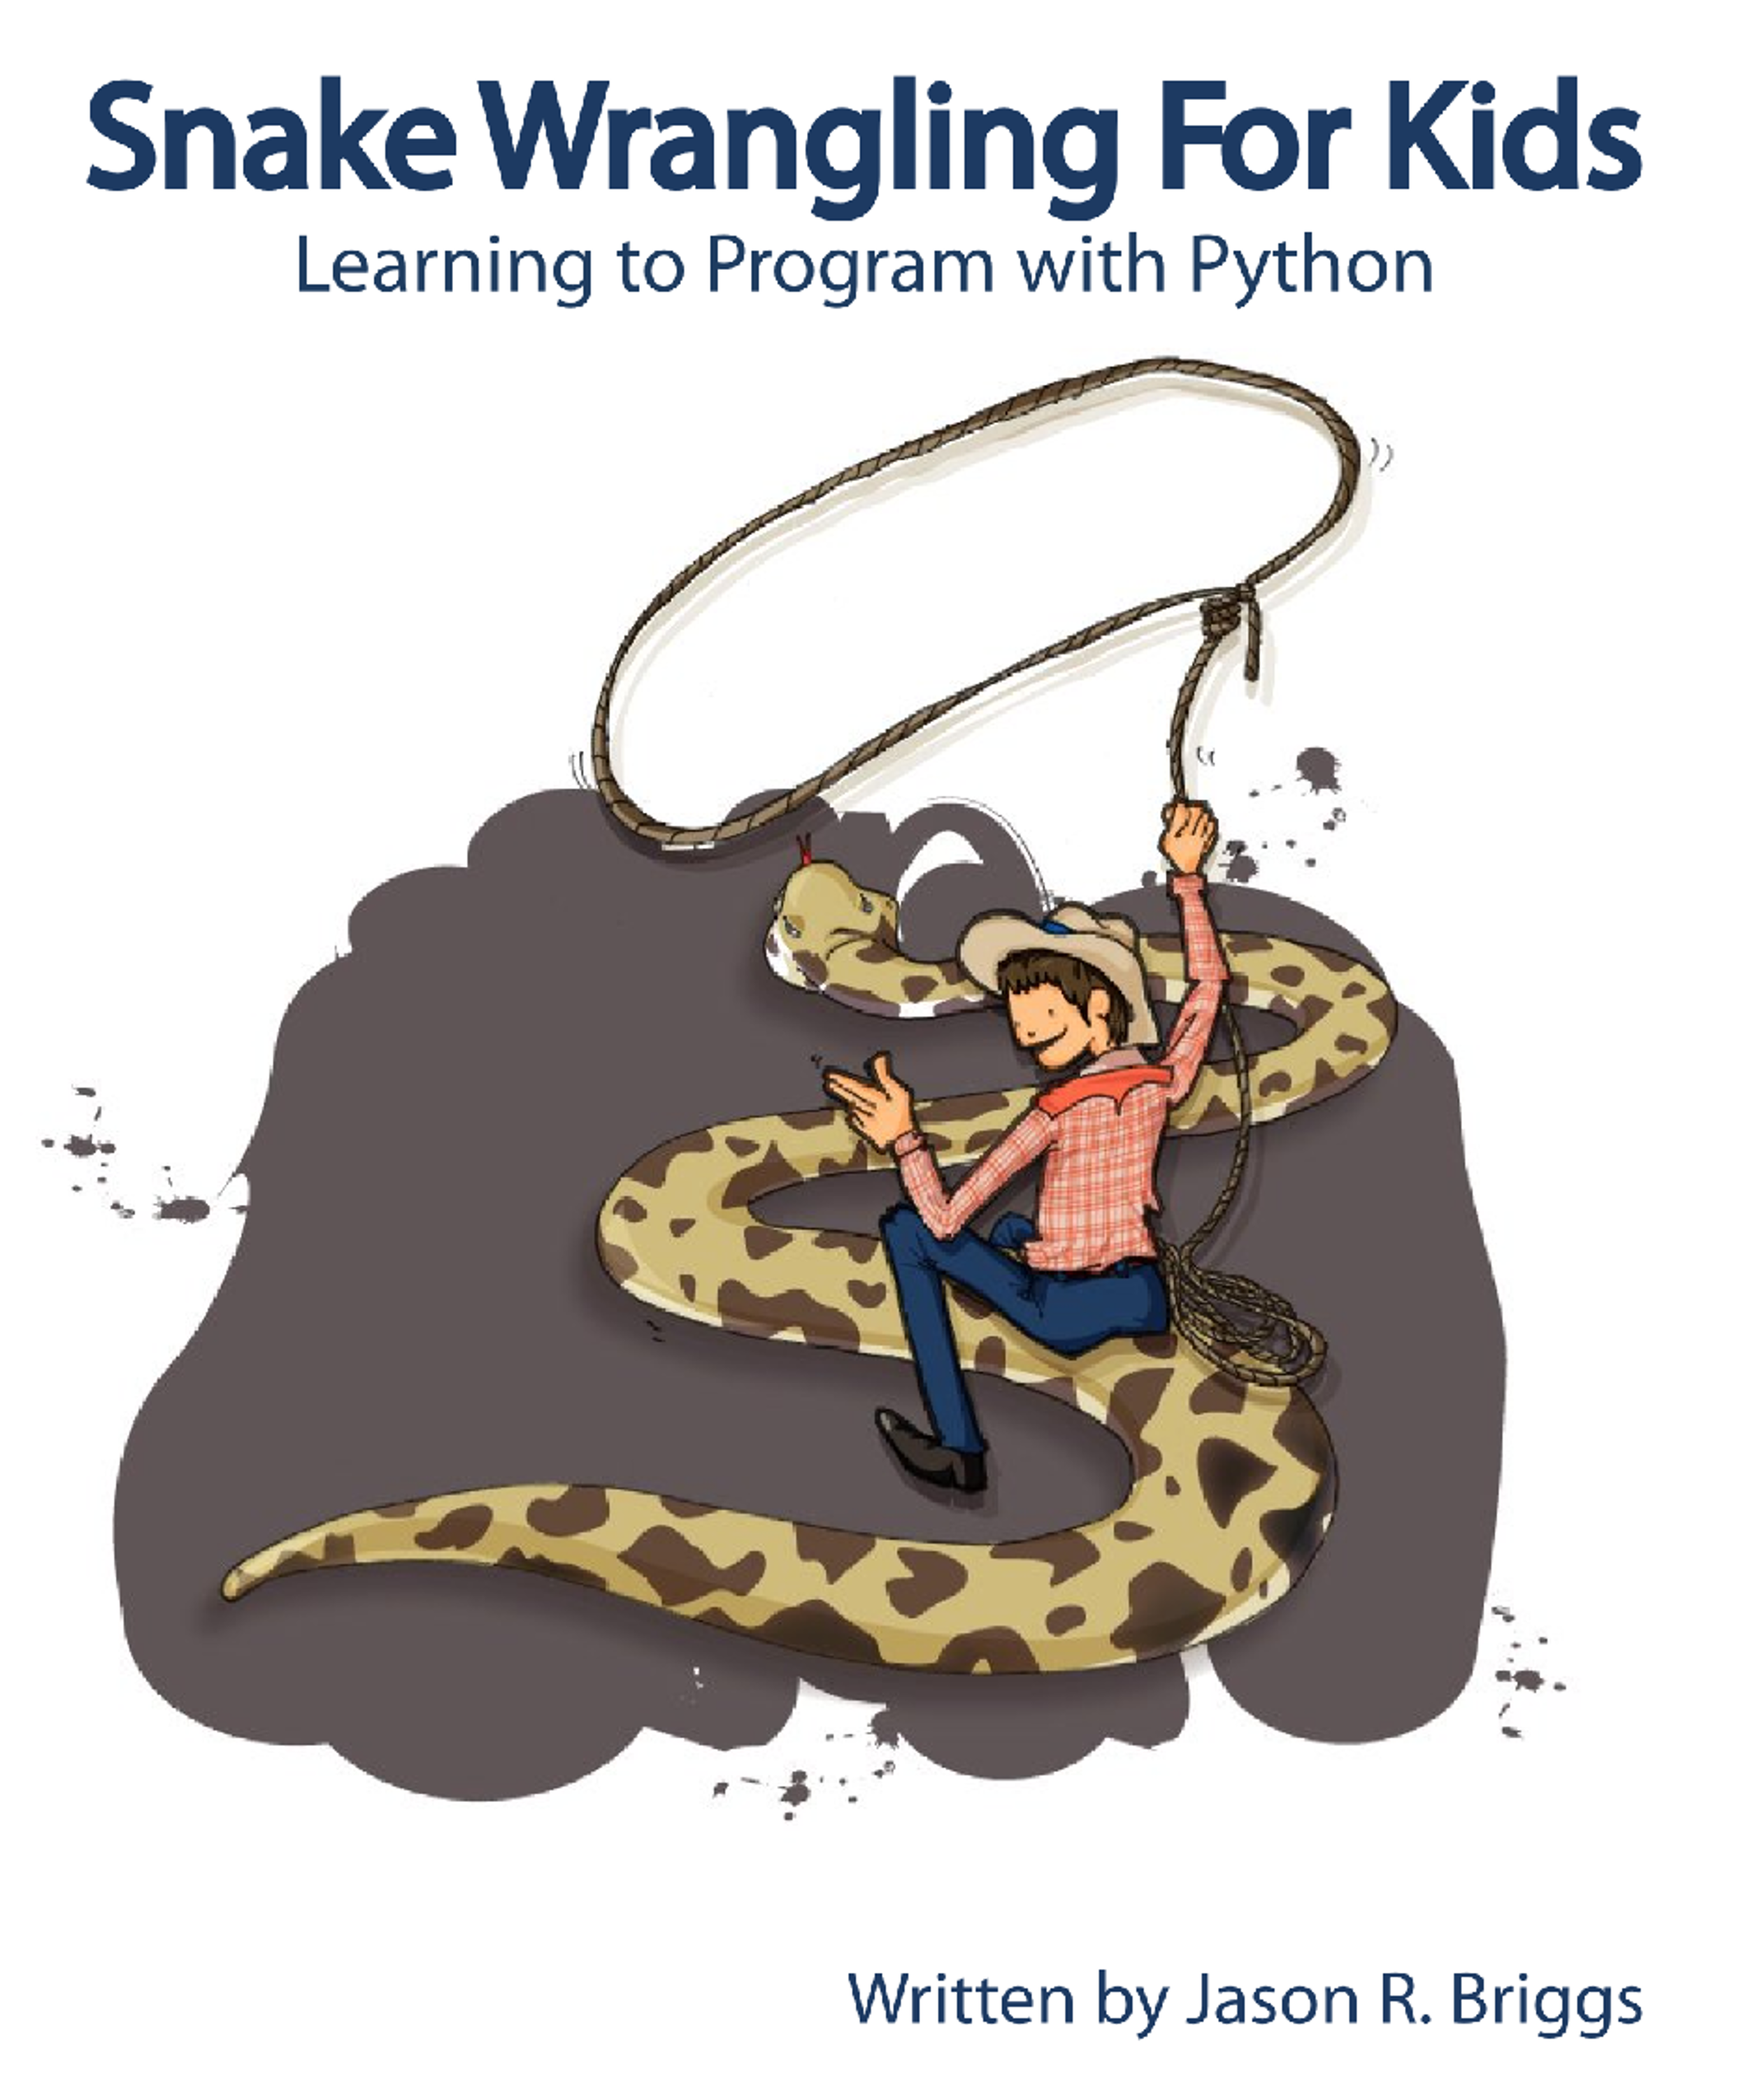
\includegraphics[width=0.9\paperwidth]{cover.eps}
\end{textblock*}
\begin{flushright}
\begin{WINDOWS}
\includegraphics[width=40mm]{windows-edition.eps} 
\end{WINDOWS}
\begin{MAC}
\includegraphics[width=40mm]{mac-edition.eps} 
\end{MAC}
\begin{LINUX}
\includegraphics[width=40mm]{linux-edition.eps} 
\end{LINUX}
\end{flushright}
\end{titlepage}

\noindent
\textsf{\emph{Snake Wrangling for Kids, Learning to Program with Python}}\\
by Jason R. Briggs\\
\\
Version 0.7.2
\\\\
Copyright \copyright 2007.\\
\\
Published by... ah, no one actually.\\
\\
Cover art and illustrations by Nuthapitol C.\\
\linebreak 
\noindent
Website:\\ \href{http://www.briggs.net.nz/log/writing/snake-wrangling-for-kids}{http://www.briggs.net.nz/log/writing/snake-wrangling-for-kids}\\ 

\noindent
Thanks To:\\
Guido van Rossum (for benevelont dictatorship of the Python language), the members of the Edu-Sig mailing list (for helpful advice and commentary), and author David Brin (the original instigator of this book).\\

\noindent
License:\\
This work is licensed under the Creative Commons Attribution-Noncommercial-Share Alike 3.0 New Zealand License. To view a copy of this license, visit\\ \href{http://creativecommons.org/licenses/by-nc-sa/3.0/nz/}{http://creativecommons.org/licenses/by-nc-sa/3.0/nz/} or send a letter to Creative Commons, 171 Second Street, Suite 300, San Francisco, California, 94105, USA.\\

\noindent
Below is a summary of the license.\\

\noindent
You are free:
\begin{itemize}
 \item \textbf{to Share} — to copy, distribute and transmit the work 
 \item \textbf{to Remix} — to adapt the work
\end{itemize}
\noindent
Under the following conditions:
\begin{description}
 \item[Attribution.] You must attribute the work in the manner specified by the author or licensor (but not in any way that suggests that they endorse you or your use of the work).
 \item[Noncommercial.] You may not use this work for commercial purposes.
 \item[Share Alike.] If you alter, transform, or build upon this work, you may distribute the resulting work only under the same or similar license to this one.
\end{description}

\noindent
For any reuse or distribution, you must make clear to others the license terms of this work.\\

\noindent
Any of the above conditions can be waived if you get permission from the copyright holder.\\

\noindent
Nothing in this license impairs or restricts the author's moral rights.\\

\mainmatter

\pagestyle{plain}

\pagenumbering{roman}
\tableofcontents

% preface.tex
% This work is licensed under the Creative Commons Attribution-Noncommercial-Share Alike 3.0 New Zealand License.
% To view a copy of this license, visit http://creativecommons.org/licenses/by-nc-sa/3.0/nz
% or send a letter to Creative Commons, 171 Second Street, Suite 300, San Francisco, California, 94105, USA.


\chapter*{Preface}\normalsize
    \addcontentsline{toc}{chapter}{Preface}
\begin{center}
{\em A Note to Parents...}
\end{center}
\pagestyle{plain}

\noindent
Dear Parental Unit or other Caregiver,

In order for your child to get started with programming, you're going to need to install Python on your computer.  This book has recently been updated to use Python 3.0--this latest version of Python is not compatible with earlier versions, so if you have an earlier version of Python installed, then you'll need to download an older release of the book.

Installing Python is a fairly straight-forward task, but there are a few wrinkles depending upon what sort of Operating System you're using.  If you've just bought a shiny new computer, have no idea what to do with it, and that previous statement has filled you with a severe case of the cold chills, you'll probably want to find someone to do this for you.  Depending upon the state of your computer, and the speed of your internet connection, this could take anything from 15 minutes to a few hours.

\begin{WINDOWS}

\noindent
First of all, go to \href{http://www.python.org}{www.python.org} and download the latest Windows installer for Python 3.  At time of writing, this is:
\begin{quote}
     \href{http://www.python.org/ftp/python/3.0/python-3.0.msi}{http://www.python.org/ftp/python/3.0/python-3.0.msi}
\end{quote}
Double-click the icon for the Windows installer (you do remember where you downloaded it to, don't you?), and then follow the instructions to install it in the default location (this is probably \emph{c:$\backslash$Python30} or something very similar).

\end{WINDOWS}

\begin{MAC}

\noindent
At time of writing, installing Python 3 on your Mac is a more complicated process than usual.  At the moment, there are no one-click install packages available.  There is information out there describing the installation process (here is a good \href{http://farmdev.com/thoughts/66/python-3-0-on-mac-os-x-alongside-2-6-2-5-etc-/}{page}), but the basic process is to download the source package and then build it yourself.  This isn't as difficult as it sounds, but you will need to follow a few steps in the Terminal.  If you find this too complicated, I recommend sticking with the \href{http://www.briggs.net.nz/log/wp-content/uploads/2008/03/swfk-mac.zip}{previous version} of this book.

\noindent
First of all, go to \href{www.python.org}{www.python.org} and download the Python source package. As of Dec 2008, the address for this download is:

\noindent
\href{http://www.python.org/ftp/python/3.0/Python-3.0.tar.bz2}{http://www.python.org/ftp/python/3.0/Python-3.0.tar.bz2}

\noindent
Start the Terminal application, and enter the following commands:

\begin{listing}
\begin{verbatim}
$ cd ~/Downloads/Python-3.0/
$ ./configure --enable-framework MACOSX_DEPLOYMENT_TARGET=10.5 --with-universal-archs=all
$ make && make test
$ sudo make frameworkinstall
\end{verbatim}
\end{listing}

\noindent
The following steps may, or may not, be necessary.  First of all type: 

\code{ls -la /Library/Frameworks/Python.framework/Versions/}

\noindent
In my case, there are only two directories shown:

\begin{listing}
\begin{verbatim}
    drwxr-xr-x  4 root  admin  136  6 Dec 23:31 .
    drwxr-xr-x  6 root  admin  204  6 Dec 23:31 ..
    drwxr-xr-x  9 root  admin  306  6 Dec 23:32 3.0
    lrwxr-xr-x  1 root  admin    3  6 Dec 23:31 Current -> 3.0
\end{verbatim}
\end{listing}

\noindent
If you have more than those two directories listed (for example)$\ldots$

\begin{listing}
\begin{verbatim}
    drwxr-xr-x  4 root  admin  136   6 Dec 23:31 .
    drwxr-xr-x  6 root  admin  204   6 Dec 23:31 ..
    drwxr-xr-x  9 root  admin  306   7 Nov 08:19 2.4
    drwxr-xr-x  9 root  admin  306  22 Mar 23:32 2.5
    drwxr-xr-x  9 root  admin  306  12 Dec 10:22 2.6
    drwxr-xr-x  9 root  admin  306   6 Dec 23:31 3.0
    lrwxr-xr-x  1 root  admin    3   6 Dec 23:31 Current -> 3.0
\end{verbatim}
\end{listing}

\noindent
$\ldots$then you may need to perform the following steps:

\begin{listing}
\begin{verbatim}
$ cd /Library/Frameworks/Python.framework/Versions/
$ sudo rm Current
$ sudo ln -s 2.5 Current
\end{verbatim}
\end{listing}

Finally, you'll want to setup Python 3 as the default, for when your child opens the Terminal application. To do this you'll need to edit the path used by Terminal--start Terminal, and then enter the following command \code{pico ~/.bash\_profile}.  This file may (or may not) exist already, and if it does, there may (or may not) already be a path set up.  In any case, at the bottom of the file, add the following:

\begin{listing}
\begin{verbatim}
export PATH="/Library/Frameworks/Python.framework/Versions/3.0/bin:${PATH}"
\end{verbatim}
\end{listing}

Save your changes, by hitting CTRL+X, and typing Y to save. If you restart the Terminal app, and type \code{python}, with any luck, you should see something similar to the following:

\begin{listing}
\begin{verbatim}
Python 3.0 (r30:67503, Dec  6 2008, 23:22:48) 
[GCC 4.0.1 (Apple Inc. build 5465)] on darwin
Type "help", "copyright", "credits" or "license" for more information.
>>>
\end{verbatim}
\end{listing}

\end{MAC}

\begin{LINUX}

\noindent
First of all, download and install the latest version of Python 3 for your distribution.  Given the large number of Linux flavours, it's impossible to give exact details on installation for each---but chances are, if you're running Linux, you already know what you're doing anyway.  In fact, you're probably insulted by the very idea of being told how to install$\ldots$anything

\end{LINUX}

\noindent
\emph{\color{BrickRed}After installation$\ldots$}

\noindent
$\ldots$You might need to sit down next to your child for the first few chapters, but hopefully after a few examples, they should be batting your hands away from the keyboard to do it themselves.  They should, at least, know how to use a text editor of some kind before they start (no, not a Word Processor, like Microsoft Word---a plain, old-fashioned text editor)---they should at least able to open and close files, create new text files and save what they're doing.  Apart from that, this book will try to teach the basics from there.
\\
\\
\noindent\\
Thanks for your time, and kind regards,
\noindent\\
THE BOOK

\pagestyle{headings}
\pagenumbering{arabic}

% ch1.tex
% This work is licensed under the Creative Commons Attribution-Noncommercial-Share Alike 3.0 New Zealand License.
% To view a copy of this license, visit http://creativecommons.org/licenses/by-nc-sa/3.0/nz
% or send a letter to Creative Commons, 171 Second Street, Suite 300, San Francisco, California, 94105, USA.


\chapter{No todas las serpientes muerden}\label{ch:notallsnakeswillsquishyou}

Existe la posibilidad de que te regalasen este libro en tu cumpleaños. O posiblemente en navidades. La tía Pili iba a regalarte unos calcetines que eran dos tallas más grandes que la tuya (que no querrías llevar ni cuando crecieras). En vez de eso, oyó a alguien hablar de este libro imprimible desde Internet, recordó que tenías uno de esos aparatos que se llaman ordenadores o algo así y que intentaste enseñarle a usarlo las últimas navidades (cosa que dejaste de hacer cuando viste que ella intentaba hablarle al ratón), y te imprimió una copia. Agradécele que no te regalase los viejos calcetines.

En vez de eso, espero que no te haya defraudado cuando salí del papel de envolver reciclado. Yo, un libro que no habla tanto como tu tía (de acuerdo, no hablo nada de nada), con un título que no augura nada bueno sobre ``Aprender$\ldots$''.
Sin embargo, entretente un rato pensando como me siento yo. Si fueras el personaje de esta novela sobre magos que está en la estantería de tu dormitorio, posiblemente yo tendría dientes... o incluso ojos. Dentro de mí tendría fotos con imágenes que se moverían, o sería capaz de hacer sonidos y quejidos fantasmales cuando abrieras mis páginas. En luga de eso, estoy impreso en páginas de tamaño folio, grapadas o tal vez aprisionadas en una carpeta. Como podría saberlo---Si no tengo ojos.
\\
\\
\emph{Daría cualquier cosa por una hermosa y afilada dentadura$\ldots$}
\\
\\
Si embargo no es tan malo como suena. Incluso aunque no pueda hablar... o morderte los dedos cuando no estás mirando... Puedo enseñarte un poquito sobre lo que hace que los ordenadores funcionen. No hablo de las piezas, con cables, conexiones, chips de ordenador y dispositivos que podrían, más que probablemente, electrocutarte en cuanto los tocaras (por eso ¡¡no los toques!!)---sino de todo aquello que por va dentro de esos cables, circuitos y chips, que es lo que hace que los ordenadores sean útiles.

\begin{wrapfigure}{r}{0.5\textwidth}
  \begin{center}
\includegraphics*[width=70mm]{electrocute.eps}
  \end{center}
\end{wrapfigure}

Es como esos pequeños pensamientos que andan dentro de tu cabeza. Si no tuvieras pensamientos estarías sentado en el suelo de tu dormitorio, con la mirada perdida hacia la puerta de tu habitación y babeando en la camiseta. Sin los \emph{programas}, los ordenadores solamente serían útiles para sujetar las puertas---e incluso para eso no serían muy útiles, porque tropezarías constantemente con ellos por la noche. Y no hay nada peor que darse un golpe en un dedo del pie en la oscuridad.
\\
\\
\emph{Solamente soy un libro, incluso yo sé eso}
\\
\\
Tu familia puede que tenga una Playstation, Xbox o Wii en la sala de estar---No son muy útiles sin programas (Juegos) para hacerlas funcionar. Tu reproductor de DVD, posiblemente tu frigorífico e incluso tu coche, todos contienen programas de ordenador para hacerlos más útiles de lo que serían sin ellos. Tu reproductor de DVD tiene programas que sirven para que pueda reproducir lo que hay en un DVD; tu frigorífico podría tener un programa simple que le asegura que no usa demasiada electricidad, pero sí la suficiente para mantener la comida fría; tu coche podría tener un ordenador con un programa para avisar al conductor que van a chocar contra algo.\\
Si supieras escribir programas de ordenador, podrías hacer toda clase de cosas útiles, Tal vez escribir tus propios juegos. Crear páginas web que hagan cosas, en lugar de estar ahí delante paradas con sus colorida apariencia. Ser capaz de programar te podría ayudar incluso con tus deberes.\\
\\
Dicho esto, vamos a hacer algo un poco más interesante.

\section{Unas pocas palabras sobre el lenguaje}

Como pasa con los humanos, con las ballenas, posiblemente con los delfines, y puede que incluso con los padres (aunque esto último se puede debatir), los ordenadores tienen su propio idioma o lenguaje. En realidad, también como con los humanos, tienen más de un idioma. Hay tantos lenguajes que casi se acaban las letras del alfabeto. A, B, C, D y E no son únicamente letras, también son nombres de lenguajes de programación (lo que prueba que los adultos no tienen imaginación, y que deberían leer un diccionario antes de darle nombre a nada).

Hay lenguajes de programación cuyo nombre viene de nombres de personas, otros cuyo nombre viene de acrónimos (las letras mayúsculas de una serie de palabras), y algunos pocos cuyo nombre proviene de algún espectáculo de televisión. Ah, y si le añades algunos simbolos más y hash (+, \#) después de un par de las letras que comenté antes---también hay un par de lenguajes de programación que se llamen así. Para complicar más las cosas, algunos de esos lenguajes son casi iguales, y sólo varían ligeramente.
\\
\\
\emph{¿Qué te dije? ¡Sin imaginación!}
\\
\\
Por fortuna, muchos de estos lenguajes ya no se usan mucho, o han desaparecido completamente; pero la lista de las diferentes formas de las que le puedes `hablar' al ordenador sigue siendo preocupantemente larga. Yo únicamente voy a comentar una de ellas---de otra manera posiblemente ni siquiera podríamos empezar.
\\
Sería mas productivo permanecer sentado en tu dormitorio babeando la camiseta$\ldots$

\section{La Orden de las Serpientes Constrictoras No Venenosas$\ldots$}

$\ldots$o Pitones, para abreviar.

Aparte de ser una serpiente, Python\index{Python} es también un lenguaje de programación. Sin embargo, el nombre no procede este reptil sin patas; en vez de eso es uno de los pocos lenguajes de programación cuyo nombre viene de un programa de televisión. Monty Python era un espectáculo de comedia Británica que fue popular en la década de los 70 (1970-1979), y que aún es popular hoy día, en realidad, para la que tienes que ser de una cierta edad para encontrarla entretenida. Cualquiera bajo una edad de unos $\ldots$ digamos 12$\ldots$ se sorprenderá de las pasiones que levanta esta comedia\footnote{Salvo por la danza de los golpes de pescado. Eso es divertido independientemente de la edad que tengas.}.

Hay algunas cosas sobre Python (el lenguaje de programación, no la serpiente, ni el espectáculo de televisión) que lo hacen extremadamente útil cuando estás aprendiendo a programar. Para nosotros, por el momento, la razón más importante es que puedes comenzar a hacer cosas realmente rápido.

Esta es la parte en la que espero que Mamá, Papá (o cualquiera que sea que esté a cargo del ordenador), hayan leído el comienzo de este libro que está etiquetado como ``Una Nota para los Padres:''

\noindent
Hay una buena manera de descubrir si realmente se la han leído:

\begin{WINDOWS}
Haz click en el botón de Inicio en la parte izquierda de la pantalla, pulsa en la opción `Todos los Programas' (que tiene un triángulo verde junto a ella), y, si todo va bien, en la lista de programas deberías ver `Python 2.5' o `Python 3.0' (o algo parecido). La Figura~\ref{fig1} te muestra lo que estás buscando. Pulsa en la opción `Python (línea de comando)' y deberías ver algo parecido a la Figura~\ref{fig2}.

\begin{figure}
\begin{center}
\includegraphics[width=80mm]{figure1.eps}
\end{center}
\caption{Python en el menú de opciones de Windows.}\label{fig1}
\end{figure}

\begin{figure}
\begin{center}
\includegraphics[width=135mm]{figure2.eps}
\end{center}
\caption{La consola de Python en Windows.}\label{fig2}
\end{figure}
\end{WINDOWS}

\begin{MAC}
En Finder, a la izquierda deberías ver un grupo denominado `Aplicaciones'. Pulsa en él, y busca un programa denominado `Terminal' (probablemente estará en una carpeta denominada `Utilidades').
Pulsa en `Terminal', y cuando se inicie, teclea python y pulsa Intro. Debería mostrarse una ventana como la de la Figura~\ref{fig3}.

\begin{figure}
\begin{center}
\includegraphics[width=85mm]{figure3.eps}
\end{center}
\caption{La consola de Python en el Mac OSX.}\label{fig3}
\end{figure}
\end{MAC}

\begin{LINUX}
Pregunta a Mamá o a Papá qué aplicación de terminales deberías usar (puede ser una llamada `Konsole', `rxvt', `xterm', o cualquier otra de la docena de diferentes programas---por eso es por lo que seguramente tendrás que preguntar). Inicia el terminal que te hayan indicado y teclea `python' (sin las comillas), y pulsa Intro. Deberías ver algo parecido a lo que se muestra en la Figura~\ref{fig4}.

\begin{figure}
\begin{center}
\includegraphics[width=80mm]{figure4.eps}
\end{center}
\caption{La consola de Python en Linux.}\label{fig4}
\end{figure}
\end{LINUX}

\subsection*{\color{BrickRed}Si descubrieras que no se han leido la sección del comienzo del libro$\ldots$}

$\ldots$porque falta algo cuando intentas seguir las instrucciones---entonces ve al comienzo del libro, y se lo pasas por delante de sus narices mientras estén intentando leer el periódico, y pon cara esperanzada. Diciendo, ``por favor por favor por favor por favor'' y así una y otra vez, hasta que resulte molesto, podría funcionar bastante bien, si tuvieras problemas en convencerles para que se levanten del sillón, puede probar otra cosa, ir al comienzo del libro y seguir las instrucciones en la Introducción para instalar Python tú mismo.

\section{Tu primer programa en Python}

Con algo de suerte, si has alcanzado este punto, has conseguido iniciar la consola de Python, que es una de las formas de ejecutar sentencias y programas. Al iniciar la consola (o después de ejecutar una sentencia), verás lo que se llama un `prompt'. En la consola de Python\index{Python console}, el prompt está formado por tres símbolos de `mayor que' ($>$) que forman una flecha apuntando a la derecha:

\begin{listing}
\begin{verbatim}
>>>
\end{verbatim}
\end{listing}

Si juntas suficientes sentencias de Python, tendrás un programa que podrás ejecutar más allá de la consola$\ldots$ pero por el momento vamos a hacer lo más simple, y teclear nuestras sentencias directamente en la consola, en el prompt ($>>>$).  Así que, por qué no comenzar tecleando lo siguiente:

\begin{listing}
\begin{verbatim}
print("Hola mundo")
\end{verbatim}
\end{listing}

Asegúrate que incluyes las comillas (eso es, estas comillas: $"$ $"$), y pulsa la tecla Intro al finalizar la línea. Si todo va bien verás en la pantalla algo como lo siguiente:

\begin{listing}
\begin{verbatim}
>>> print("Hola mundo")
Hola mundo
\end{verbatim}
\end{listing}

El prompt reaparece, con el fin de hacerte saber que la consola de Python está lista para aceptar más sentencias.

\noindent
¡Enhorabuena! Acabas de crear tu primer programa Python.  \code{print} es una función que se encarga de escribir en la consola todo lo que se encuentre dentro de los paréntesis--la utilizaremos repetidamente más adelante.

\section{Tu segundo programa en Python$\ldots$¿Otra vez lo mismo?}

Los programas en Python no serían nada útiles si tuvieras que teclear las sentencias cada vez que quisieras hacer algo---o si escribieras programas para alguien, y tuvieran que teclearlo cada vez antes de que pudieran usarlo. 
El Procesador de Textos que uses para escribir las tareas del cole, tiene probablemente entre 10 y 100 millones de líneas de código (sentencias). Dependiendo de cuantas líneas imprimieras en una página (y si las imprimes o no por ambas caras del papel), esto supondría alrededor de 400.000 páginas en papel$\ldots$ o una pila de papel de unos 40 metros de alto.
Imagínate cuando tuvieras que traer esta aplicación a casa desde la tienda, habría que hacer unos cuantos viajes con el coche, para llevar tantos papeles$\ldots$

$\ldots$y mejor que no sople el viento mientras transportas esas pilas de papel. Por fortuna, existe una alternativa a tener que teclearlo todo cada vez---o nadie podría hacer nada.

\begin{center}
\includegraphics*[width=85mm]{pullinghair.eps}
\end{center}

\begin{WINDOWS}
Abre el Block de Notas (Notepad) (Pulsa en el menú de Inicio, Todos los Programas: debería estar en el submenú de Accesorios), y teclea la sentencia print exactamente igual que lo hiciste antes en la consola:

\begin{listing}
\begin{verbatim}
print("Hola mundo")
\end{verbatim}
\end{listing}

Pulsa en el menú Archivo (en el Block de Notas), luego Guardar, y cuando te pregunte por qué nombre darle al fichero, llámalo \emph{hola.py} y grábalo en tu Escritorio. Haz doble click en el icono que aparece en el Escritorio con el nombre hola.py (ver Figura~\ref{fig5}) y durante un breve momento se mostrará una ventana con la consola. Desaparecerá demasiado rápido como para ver lo que pone, pero lo que se mostrará en pantalla en esas décimas de segundo será Hola mundo---volveremos a esto más tarde para comprobar que es verdad lo que digo.\\

\begin{figure}
\begin{center}
\includegraphics[width=58mm]{figure5.eps}
\end{center}
\caption{El icono hola.py en el Escritorio de Windows.}\label{fig5}
\end{figure}
\end{WINDOWS}

\begin{MAC}
Abre el Editor de Textos pulsando sobre su icono. Puede estar en el Dock de la parte de abajo de la pantalla \includegraphics*[width=12mm]{textedit-icon.eps}, o busca este icono \includegraphics*[width=19mm]{textedit-icon2.eps} en la lista de Aplicaciones en Finder.  Una vez abierto, teclea la sentencia print de la misma forma que hisciste antes en la consola:

\begin{listing}
\begin{verbatim}
print("Hola mundo")
\end{verbatim}
\end{listing}

Haz click en el menú de Archivo, luego pulsa Guardar, y cuando te pregunte por un nombre de fichero, llámalo hola.py y guárdalo en tu directorio home (el directorio home está a la izquierda bajo Lugares--pregunta a Mamá o a Papá para que te ayuden a encontrarlo).

Abre la aplicación `Terminal' de nuevo--se iniciará automáticamente en tu directorio home--y teclea lo siguiente:

\begin{listing}
\begin{verbatim}
python hola.py
\end{verbatim}
\end{listing}

Deberías ver Hola mundo escrito en la ventana exactamente como cuando tecleaste la sentencia en la consola de Python.

\end{MAC}

\begin{LINUX}
Abre un editor de texto (de nuevo tendrás que preguntar a Mamá o a Papá cual usar), luego teclea la sentencia print exactamente como la tecleaste en la consola:

\begin{listing}
\begin{verbatim}
print("Hola mundo")
\end{verbatim}
\end{listing}

Pulsa en el menú Archivo, luego Guardar, y cuando te pregunte por el nombre del fichero, llámalo hola.py y sálvalo en tu carpeta Home (puede que haya un icono llamado `Home' en algún lugar en el diálogo que aparece para Guardar). Luego abre la aplicación de terminal (de nuevo Konsole, rxvt, etc... la que usamos antes), y teclea:

\begin{listing}
\begin{verbatim}
python hola.py
\end{verbatim}
\end{listing}

Deberías ver Hola mundo escrito en la ventana exactamente como cuando tecleaste la sentencia en la consola de Python (ver Figura~\ref{fig9}).

\begin{figure}
\begin{center}
\includegraphics[width=75mm]{figure9.eps}
\end{center}
\caption{Ejecutando en Linux un programa python grabado en un fichero de texto.}\label{fig9}
\end{figure}
\end{LINUX}

Como ves la gente que creó Python era gente decente, te ha librado de tener que teclear lo mismo una y otra vez y otra vez y otra vez y otra vez. Como pasó en los años ochenta. No, lo digo en serio---lo hicieron. Ve y pregunta a tu Padre si alguna vez tuvo un ZX81 cuando era más joven\\

\noindent
Si lo tuvo puedes señalarle con el dedo y reirte.\\

\noindent
Créeme. No lo entenderás. Pero él sí.\footnote{El Sinclair ZX81, vendido en la década de 1980 fue uno de los primeros ordenadores para el hogar que se vendía a un precio asequible. Un gran número de jóvenes se volvieron `locos' tecleando el código de juegos que venían impresos en revistas sobre el ZX81---únicamente para descubrir, después de horas de teclear, que esos malditos juegos nunca funcionaban bien.}

\noindent
\emph{De todos modos, prepárate para salir corriendo.}

\subsection*{\color{BrickRed}El Final del Comienzo}

Bienvenido al maravilloso mundo de la Programación. Hemos empezado con una aplicación sencillita `Hola mundo'---todo el mundo comienza con eso, cuando empiezan a programar.
En el siguiente capítulo comenzaremos a hacer cosas más útiles con la consola de Python y empezaremos a ver lo que hace falta para hacer un programa.

\newpage

% ch2.tex
% This work is licensed under the Creative Commons Attribution-Noncommercial-Share Alike 3.0 New Zealand License.
% To view a copy of this license, visit http://creativecommons.org/licenses/by-nc-sa/3.0/nz
% or send a letter to Creative Commons, 171 Second Street, Suite 300, San Francisco, California, 94105, USA.


\chapter{8 multiplied by 3.57 equals$\ldots$}\label{ch:8multipliedby3.57}

What is 8 multiplied by 3.57?  You'd have to use a calculator, wouldn't you?  Well perhaps you're extremely smart and can do multiplication of fractions in your head---but that's not the point.  You can also do the same thing with the Python console. Start up the console again (see Chapter~\ref{ch:notallsnakeswillsquishyou} for more information, if you've skipped ahead for some strange reason), and once you see the prompt, type 8$*$3.57 and press the Enter key:

\begin{listing}
\begin{verbatim}
Python 2.5.1 (r251:54863, May 2 2007, 16:56:35)
Type "help", "copyright", "credits" or "license" for more information.
>>> 8 * 3.57
28.559999999999999
\end{verbatim}
\end{listing}

The star (*), or asterisk key (shift 8 on some keyboards), is used for multiplication\index{multiplication}, instead of the normal times symbol (\textsf{X}) that you use at school (using the star key is necessary, otherwise how would the computer know whether you meant the letter \emph{x} or the multiplication symbol \textsf{X} ?).

How about an equation that's a bit more useful?

Suppose you do chores once a week, for which you get \$5 pocket money, and you have a paper round which you do 5 times a week and get \$30---how much money would you earn in a year?

\begin{figure}[t]
\begin{center}
\fbox{\colorbox{PaleBlue}{\parbox{.75\linewidth} {
\subsection*{Python is broken!?!?}

If you just picked up a calculator and entered 8 x 3.57 the answer showing on the display will be:\\

\textsf{
28.56\\
}

\noindent
Why is Python different?  Is it broken?\\

\noindent
Actually, no. The reason can be found in the way floating point\index{floating point} (fractional numbers with a decimal place) numbers are handled by the computer.  It's a complicated and somewhat confusing problem for beginners, so it's best to just remember that when you're working with fractions (i.e. with a decimal place on a number), \emph{sometimes} the result won't be exactly what you were expecting. This is true for multiplication, division, addition or subtraction.
}}}
\end{center}
\end{figure}

If we were writing that on paper, we might write something like:
\begin{verbatim}
(5 + 30) x 52
\end{verbatim}

Which is \$5 + \$30 multiplied by 52 weeks in a year.  \begin{samepage}Of course, we're smart, and we know that 5 + 30 is 35, so the equation is really:

\begin{verbatim}
35 x 52
\end{verbatim}
\end{samepage}

Which is easy enough to do in a calculator, or on paper.  But we can do all of these calculations with the console as well:

\begin{listing}
\begin{verbatim}
>>> (5 + 30) * 52
1820
>>> 35 * 52
1820
\end{verbatim}
\end{listing}

So, what if you spend \$10 each week?  How much do you have left at the end of the year?  We could write the equation on paper a couple of different ways, but let's just type it into the console:

\begin{listing}
\begin{verbatim}
>>> (5 + 30 - 10) * 52
1300
\end{verbatim}
\end{listing}

That's \$5 and \$30 minus \$10 multiplied by 52 weeks in the year1.  And you'd have \$1300 left at the end of the year. Okay, so that's not looking all that useful so far.  We can do all of that with a calculator.  But we'll come back to this later and show how to make it much more useful.

You can do multiplication\index{multiplication} and addition\index{addition} (obviously), and subtraction\index{subtraction} and division\index{division} in the Python console, along with a bunch of other maths operations that we won't go into now.  For the moment the basic maths symbols for Python (actually they're called operators\index{operators}) are:

\begin{center}
\begin{tabular}{|c|c|}
\hline
+ & Addition \\
\hline
- & Subtraction \\
\hline
* & Multiplication \\
\hline
/ & Division \\
\hline
\end{tabular}
\end{center}

The reason the forward-slash (/) is used for division, is that it would be rather difficult to draw a division line (plus they didn't bother to put a division symbol $\div$ on the computer keyboard) as you're supposed to use for written equations.  For example if you had 100 eggs and 20 boxes, you might want to know how many eggs would go in each box, so you'd show dividing 100 into 20, by writing the following equation:

\begin{displaymath}
\frac{100}{200}
\end{displaymath}

Or if you know about long division, you might write it out fully like this:

\begin{displaymath}
\longdiv{100}{20}
\end{displaymath}

Or you might even write it like this:

\begin{displaymath}
100 \div 20
\end{displaymath}

However, in Python terms you would just type it as ``100 / 20''.

\emph{Which is much easier, I think.  But then, I'm a book---what do I know?}

\section{Use of brackets and ``Order of Operations''}\index{order of operations}

We use brackets in a programming language to control what is called ``Order of Operations''.  An operation is the use of an operator (one of those symbols in the table above).  There are more operators than those basic symbols, but for that simple list (addition, subtraction, multiplication and division), it's enough to know that multiplication and division both have a higher order than addition and subtraction.  Which means you do the multiplication or division part of an equation before you do the addition or subtraction part.  In the following equation, all the operators are addition (+), the numbers are added in order:

\begin{listing}
\begin{verbatim}
>>> print 5 + 30 + 20
55
\end{verbatim}
\end{listing}

\noindent
Similarly, in this equation, there are only addition and subtraction operators, so again Python considers each number in the order it appears:

\begin{listing}
\begin{verbatim}
>>> print 5 + 30 - 20
15
\end{verbatim}
\end{listing}

\noindent
But in the following equation, there is a multiplication operator, so the numbers 30 and 20 are considered first.  The equation is another way of saying, ``multiply 30 by 20, then add 5 to the result'' (multiplication first, because it has a higher order than addition):

\begin{listing}
\begin{verbatim}
>>> print 5 + 30 * 20
605
\end{verbatim}
\end{listing}

\noindent
So what happens when we add brackets?  The following equation shows the result:

\begin{listing}
\begin{verbatim}
>>> print (5 + 30) * 20
700
\end{verbatim}
\end{listing}

\noindent
Why is the number different?  Because brackets control the order of operations.  With brackets, Python knows to do calculate using the operators in the brackets first, then do the operators outside.  So that equation is another way of saying, ``add 5 and 30, then multiply the result by 20''.
The use of brackets can become more complicated.  There can be brackets inside brackets:

\begin{listing}
\begin{verbatim}
>>> print ((5 + 30) * 20) / 10
70
\end{verbatim}
\end{listing}

\noindent
In this case, Python evaluates the \textbf{inner} most brackets first, then the outer brackets, and then the other operator.  So this equation is a way of saying, ``add 5 and 30, then multiply the result by 20, finally divide that result by 10''.  The result without brackets is again slightly different:

\begin{listing}
\begin{verbatim}
>>> 5 + 30 * 20 / 10
65
\end{verbatim}
\end{listing}

In this case 30 is multiplied by 20 first, then the result is divided by 10, finally 5 is added to the final result.

\emph{Remember that multiplication and division always go before addition and subtraction, unless brackets are used to control the order of operations.}

\section{There's nothing so fickle as a variable}\index{variable}

A `variable' is a programming term used to describe a place to store things.  The `things' can be numbers, or text, or lists of numbers and text---and all sorts of other items too numerous to go into here.  For the moment, let's just think of a variable as something a bit like a mailbox.

\begin{center}
\includegraphics*[width=76mm]{girlbubble.eps}
\end{center}

You can put things (such as a letter or a package) in a mailbox, just as you can put things (numbers, text, lists of numbers and text, etc, etc, etc) in a variable.  This mailbox idea is the way many programming languages work.  But not all.

In Python, variables are slightly different.  Rather than being a mailbox with things in it, a variable is more like a label which is stuck on the on the outside of the mailbox.  We can pull that label off and stick it on something else, or even tie the label (perhaps with a piece of string) to more than one thing. We create a variable by giving it a name, using an equals sign (=), then telling Python what we want that name to point to.  For example:

\begin{listing}
\begin{verbatim}
>>> fred = 100
\end{verbatim}
\end{listing}

We've just created a variable called `fred' and said that it points to the number 100.  It's a bit like telling Python to remember that number because we want to use it later.  To find out what a variable is pointing at, we can just type `print' in the console, followed by the variable name, and hit the Enter key.  For example:

\begin{listing}
\begin{verbatim}
>>> fred = 100
>>> print fred
100
\end{verbatim}
\end{listing}

We can also tell Python we want the variable \code{fred} to point at something else:

\begin{listing}
\begin{verbatim}
>>> fred = 200
>>> print fred
200
\end{verbatim}
\end{listing}

\noindent
On the first line we say we now want fred to point at the number 200.  Then, in the second line, we ask what fred is pointing at just to prove it changed. We can also point more than one name at the same item:

\begin{listing}
\begin{verbatim}
>>> fred = 200
>>> john = fred
>>> print john
200
\end{verbatim}
\end{listing}

In the code above, we're saying that we want the name (or label) \code{john} to point at the same thing \code{fred} is pointing to.
Of course, `fred' isn't a very useful name for a variable.  It doesn't tell us anything about what it's used for.  A mailbox is easy---you use a mailbox for mail.  But a variable can have a number of different uses, and can point at a whole bunch of different things, so we usually want something more informative as its name.
\par
Suppose you started up the Python console, typed `fred = 200', then went away---spent 10 years climbing Mount Everest, crossing the Sahara desert, bungy-jumping off a bridge in New Zealand, and finally, sailing down the Amazon river---when you came back to your computer, would you remember what that number 200 meant (and what it was for)?

\noindent
\emph{I don't think I would.}

\noindent
I just made it up now, and I have no idea what `fred = 200' means (other than a \emph{name} pointing at the number \emph{200}).  So after 10 years, you'll have absolutely no chance of remembering.
\par
Aha!  But, what if we called our variable: \emph{number\_of\_students}.

\begin{listing}
\begin{verbatim}
>>> number_of_students = 200
\end{verbatim}
\end{listing}

We can do that because variable names can be made up of letters, numbers and (\_) underscores---although they cannot start with a number.  If you come back after 10 years, `number\_of\_students' still makes sense.  You can type:

\begin{listing}
\begin{verbatim}
>>> print number_of_students
200
\end{verbatim}
\end{listing}

\noindent
And you'll immediately know that we're talking about 200 students.  It's not always important to come up with meaningful names for variables.  You can use anything from single letters (such as `a') to large sentences; and sometimes, if you're doing something quick, a simple and short variable name is just as useful.  It depends very much upon whether you want to be able to look at that variable name later and figure out what on earth you were thinking at the time you typed it in.

\begin{listing}
\begin{verbatim}
this_is_also_a_valid_variable_name_but_perhaps_not_very_useful
\end{verbatim}
\end{listing}

\section{Using Variable}\index{Variables}

Now we know how to create a variable, how do we use it?  Remember that equation we came up with earlier?  The one to work out how much money you'd have left at the end of the year, if you earned \$5 a week doing chores, \$30 a week on a paper round, and spent \$10 per week.  So far we have:

\begin{listing}
\begin{verbatim}
>>> print (5 + 30 - 10) * 52
1300
\end{verbatim}
\end{listing}

\noindent
What if we turn the first 3 numbers into variables?  Try typing the following:

\begin{listing}
\begin{verbatim}
>>> chores = 5
>>> paper_round = 30
>>> spending = 10
\end{verbatim}
\end{listing}

\noindent
We've just created variables named `chores', `paper\_round' and `spending'.  We can then re-type the equation to get:

\begin{listing}
\begin{verbatim}
>>> print (chores + paper_round - spending) * 52
1300
\end{verbatim}
\end{listing}

Which gives the exact same answer.  What if you get \$2 more per week, for doing extra chores.  Change the `chores' variable to 7, then hit the up-arrow key ($\uparrow$) on your keyboard a couple of times, until the equation re-appears, and hit the Enter key:

\begin{listing}
\begin{verbatim}
>>> chores = 7
>>> print (chores + paper_round - spending) * 52
1404
\end{verbatim}
\end{listing}

That's a lot less typing to find out that you now end up with \$1404 at the end of the year.  You can try changing the other variables, then hit the up-arrow to perform the calculation again, and see what effect it has.

\begin{listing}
\begin{verbatim}
If you spend twice as much money per week:
>>> spending = 20
>>> print (chores + paper_round - spending) * 52
884
\end{verbatim}
\end{listing}

You're only left with \$884 savings at the end of the year. This is still only slightly useful.  We haven't hit really useful yet.  But for the moment, it's enough to understand that variables are used to store things.

\noindent
\emph{Think of a mailbox with a label on it!}

\section{A Piece of String?}\index{strings}

If you're paying attention, and not just skimming through looking for the good bits, you might remember I mentioned that variables can be used for all sorts of things---not just numbers. In programming, most of the time we call text a `string'. Which might seem a bit weird; but if you think that text is just `stringing together' (or joining together) a bunch of letters, perhaps it might make a little more sense.

\noindent
\emph{Then again, perhaps it doesn't.}

In which case, all you need to know, is that a string is just a bunch of letters and numbers and other symbols put together in some meaningful way. All the letters, and numbers, and symbols in this book could make up a string.  Your name could be a string.  So could your home address.  The first Python program we created in Chapter \ref{ch:notallsnakeswillsquishyou}, used a string: `Hello World'.
\par
In Python, we create a string by putting quotes around the text.  So we can take our useless \code{fred} variable, and put a string inside it like this:

\begin{listing}
\begin{verbatim}
>>> fred = "this is a string"
\end{verbatim}
\end{listing}

\noindent
And we can see what's inside the \code{fred} variable, by typing \code{print fred}:

\begin{listing}
\begin{verbatim}
>>> print fred
this is a string
\end{verbatim}
\end{listing}

\noindent
We can also use single-quotes to create a string:

\begin{listing}
\begin{verbatim}
>>> fred = 'this is yet another string'
>>> print fred
this is yet another string
\end{verbatim}
\end{listing}

However, if you try to type more than one line of text for your string using a single quote (') or double quote ("), you'll get an error message in the console. For example, type the following line and hit Enter, and you'll get a fairly scary error message similar to the following:

\begin{listing}
\begin{verbatim}
>>> fred = "this is two
  File "<stdin>", line 1
    fred = "this is two
                      ^
SyntaxError: EOL while scanning single-quoted string
\end{verbatim}
\end{listing}

\index{multi-line string}We'll talk more about errors later, but for the moment, if you want more than one line of text, you can use 3 single quotes:

\begin{listing}
\begin{verbatim}
>>> fred = '''this is two
... lines of text in a single string'''
\end{verbatim}
\end{listing}

\noindent
Print out the contents to see if it worked:

\begin{listing}
\begin{verbatim}
>>> print fred
this is two
lines of text in a single string
\end{verbatim}
\end{listing}

By the way, you'll see those 3 dots (...) quite a few times when you're typing something that continues onto another line (like a multi line string).  In fact, you'll see it a lot more as we continue.

\section{Tricks with Strings}\label{trickswithstrings}

Here's an interesting question:  what's 10 * 5 (10 times 5)?  The answer is, of course, 50.

\noindent
\emph{All right, that's not an interesting question at all.}

But what is 10 * 'a' (10 times the letter a)?  It might seem like a nonsensical question, but here's the answer from the World of Python:

\begin{listing}
\begin{verbatim}
>>> print 10 * 'a'
aaaaaaaaaa
\end{verbatim}
\end{listing}

This works with more than just single character strings:

\begin{listing}
\begin{verbatim}
>>> print 20 * 'abcd'
abcdabcdabcdabcdabcdabcdabcdabcdabcdabcdabcdabcdabcdabcdabcdabcdabcdabcdabcdabcd
\end{verbatim}
\end{listing}

Another trick with a string, is embedding values.  You can do this by using \%s, which is like a marker (or a placeholder) for a value you want to include in a string.  It's easier to explain with an example:

\begin{listing}
\begin{verbatim}
>>> mytext = 'I am %s years old'
>>> print mytext % 12
I am 12 years old
\end{verbatim}
\end{listing}

In the first line, the variable mytext is created with a string containing some words and a placeholder (\%s).  The \%s is a little beacon saying ``replace me with something'' to the Python console.  So on the next line, when we call print mytext, we use the \% symbol, to tell Python to replace the marker with the number 12. We can reuse that string and pass in different values:

\begin{listing}
\begin{verbatim}
>>> mytext = 'Hello %s, how are you today?'
>>> name1 = 'Joe'
>>> name2 = 'Jane'
>>> print mytext % name1
Hello Joe, how are you today?
>>> print mytext % name2
Hello Jane, how are you today?
\end{verbatim}
\end{listing}

In the above example, 3 variables (mytext, name1 and name2) are created---the first includes the string with the marker.  Then we can print the variable `mytext', and again use the \% operator to pass in variables `name1' and `name2'.  You can use more than one placeholder:

\begin{listing}
\begin{verbatim}
>>> mytext = 'Hello %s and %s, how are you today?'
>>> print mytext % (name1, name2)
Hello Joe and Jane, how are you today?
\end{verbatim}
\end{listing}

When using more than one marker, you need to wrap the replacement values with brackets---so (name1, name2) is the proper way to pass 2 variables. A set of values surrounded by brackets (the round ones, not the square ones) is called a \emph{tuple}, and is a little bit like a list, which we'll talk about next.

\section{Not quite a shopping list}\index{lists}

Eggs, milk, cheese, celery, peanut butter, and baking soda.  Which is not quite a full shopping list, but good enough for our purposes. If you wanted to store this in a variable you could create a string:

\begin{listing}
\begin{verbatim}
>>> shopping_list = 'eggs, milk, cheese, celery, peanut butter, baking soda'
>>> print shopping_list
eggs, milk, cheese, celery, peanut butter, baking soda
\end{verbatim}
\end{listing}

Another way would be to create a `list', which is a special kind of object in Python:

\begin{listing}
\begin{verbatim}
>>> shopping_list = [ 'eggs', 'milk', 'cheese', 'celery', 'peanut butter', 'baking soda' ]
>>> print shopping_list
['eggs', 'milk', 'cheese', 'celery', 'peanut butter', 'baking soda']
\end{verbatim}
\end{listing}

This is more typing, but it's also more useful.  We could print the 3rd item in the list by using its position (called its index position), inside square brackets []:

\begin{listing}
\begin{verbatim}
>>> print shopping_list[2]
cheese
\end{verbatim}
\end{listing}

Lists start at index position 0---so the first item in a list is 0, the second is 1, the third is 2.  That doesn't make a lot of sense to most people, but it does to programmers.  Pretty soon, when you walk up some stairs you'll start counting with zero rather than one.  That will really confuse your little brother or sister.
\par
We can show all the items from the 3rd item up to the 5th in the list, by using a colon inside the square brackets:

\begin{listing}
\begin{verbatim}
>>> print shopping_list[2:5]
['cheese', 'celery', 'peanut butter']
\end{verbatim}
\end{listing}

[2:5] is the same as saying that we are interested in items from index position 2 up to (but not including) index position 5.  And, of course, because we start counting with 0, the 3rd item in the list is actually number 2, and the 5th item is actually number 4. Lists can be used to store all sorts of items.  They can store numbers:

\begin{listing}
\begin{verbatim}
>>> mylist = [ 1, 2, 5, 10, 20 ]
\end{verbatim}
\end{listing}

\noindent
And strings:

\begin{listing}
\begin{verbatim}
>>> mylist = [ 'a', 'bbb', 'ccccccc', 'ddddddddd' ]
\end{verbatim}
\end{listing}

\noindent
And mixtures of numbers and strings:

\begin{listing}
\begin{verbatim}
>>> mylist = [1, 2, 'a', 'bbb']
>>> print mylist
[1, 2, 'a', 'bbb']
\end{verbatim}
\end{listing}

\noindent
And even lists of lists:

\begin{listing}
\begin{verbatim}
>>> list1 = [ 'a', 'b', 'c' ]
>>> list2 = [ 1, 2, 3 ]
>>> mylist = [ list1, list2 ]
>>> print mylist
[['a', 'b', 'c'], [1, 2, 3]]
\end{verbatim}
\end{listing}

In the above example, a variable called `list1' is created with 3 letters, `list2' is created with a 3 numbers, and `mylist' is created using list1 and list2. Things can get rather confusing, rather quickly, if you start creating lists of lists of lists of lists$\ldots$ but luckily there's not usually much need for making things that complicated in Python. Still it is handy to know that you can store all sorts of items in a Python list.

\noindent
\emph{And not just your shopping.}

\subsection*{\color{BrickRed}Replacing items}\index{lists!replacing}

We can replace an item in the list, by setting its value in a similar way to setting the value of a normal variable. For example, we could change celery to lettuce by setting the value in index position 3:

\begin{listing}
\begin{verbatim}
>>> shopping_list[3] = 'lettuce'
>>> print shopping_list
['eggs', 'milk', 'cheese', 'lettuce', 'peanut butter', 'baking soda']
\end{verbatim}
\end{listing}

\subsection*{\color{BrickRed}Adding more items...}\index{lists!appending}

We can add items to a list by using a method called `append'.  A method is an action or command that tells Python that we want to do something.  We'll talk more about methods later, but for the moment, to add an item to our shopping list, we can do the following:

\begin{listing}
\begin{verbatim}
>>> shopping_list.append('chocolate bar')
>>> print shopping_list
['eggs', 'milk', 'cheese', 'lettuce', 'peanut butter', 'baking soda', 'chocolate bar']
\end{verbatim}
\end{listing}

Which, if nothing else, is certainly an improved shopping list.

\subsection*{\color{BrickRed}$\ldots$and removing items}\index{lists!removing}

We can remove items from a list by using the command `del' (short for delete).  For example, to remove the 6th item in the list (baking soda):

\begin{listing}
\begin{verbatim}
>>> del shopping_list[5]
>>> print shopping_list
['eggs', 'milk', 'cheese', 'lettuce', 'peanut butter', 'chocolate bar']
\end{verbatim}
\end{listing}

Remember that positions start at zero, so shopping\_list[5] actually refers to the 6th item.

\subsection*{\color{BrickRed}2 lists are better than 1}\index{lists!joining}

We can join lists together by adding them, as if we were adding two numbers:

\begin{listing}
\begin{verbatim}
>>> list1 = [ 1, 2, 3 ]
>>> list2 = [ 4, 5, 6 ]
>>> print list1 + list2
[1, 2, 3, 4, 5, 6]
\end{verbatim}
\end{listing}

\noindent
We can also add the two lists and set the result to another variable:

\begin{listing}
\begin{verbatim}
>>> list1 = [ 1, 2, 3 ]
>>> list2 = [ 4, 5, 6 ]
>>> list3 = list1 + list2
>>> print list3
[1, 2, 3, 4, 5, 6]
\end{verbatim}
\end{listing}

\noindent
And you can multiply a list in the same way we multiplied a string:

\begin{listing}
\begin{verbatim}
>>> list1 = [ 1, 2 ]
>>> print list1 * 5
[1, 2, 1, 2, 1, 2, 1, 2, 1, 2]
\end{verbatim}
\end{listing}

\noindent
In the above example, multiplying list1 by five is another way of saying ``repeat list1 five times''. However, division (/) and subtraction (-) don't make sense when working with lists, so you'll get errors when trying the following examples:

\begin{listing}
\begin{verbatim}
>>> list1 / 20
Traceback (most recent call last):
  File "<stdin>", line 1, in <module>
TypeError: unsupported operand type(s) for /: 'list' and 'int'
\end{verbatim}
\end{listing}

\noindent
or:

\begin{listing}
\begin{verbatim}
>>> list1 - 20
Traceback (most recent call last):
  File "<stdin>", line 1, in <module>
TypeError: unsupported operand type(s) for -: 'type' and 'int'
\end{verbatim}
\end{listing}

\noindent
You'll get a rather nasty error message.

\section{Tuples and Lists}\label{tuplesandlists}\index{tuples}

A tuple (mentioned earlier) is a little bit like a list, but rather than using square brackets, you use round brackets---e.g. `(' and `)'.  You can use tuples in a similar way to a list:

\begin{listing}
\begin{verbatim}
>>> t = (1, 2, 3)
>>> print t[1]
2
\end{verbatim}
\end{listing}

The main difference is that, unlike lists, tuples can't change, once you've created them.  So if you try to replace a value like we did earlier with the list, you'll get another error message:

\begin{listing}
\begin{verbatim}
>>> t[0] = 4
Traceback (most recent call last):
  File "<stdin>", line 1, in ?
TypeError: 'tuple' object does not support item assignment
\end{verbatim}
\end{listing}

That doesn't mean you can't change the variable containing the tuple to something else.  For example, this code will work fine:

\begin{listing}
\begin{verbatim}
>>> myvar = (1, 2, 3)
>>> myvar = [ 'a', 'list', 'of', 'strings' ]
\end{verbatim}
\end{listing}

First we create the variable \code{myvar} pointing to a tuple of 3 numbers.  Then we change \code{myvar} to point at a list of strings. This might be a bit confusing at first.  But think of it like lockers in a school.  Each locker has a name tag on it. You put something in the locker, close the door, lock it, then throw away the key.  You then peel the name tag off, wander over to another empty locker, and stick something else in that (but this time you keep the key).  A tuple is like the locked locker.  You can't change what's inside it.  But you can take the label off and stick it on an unlocked locker, and then put stuff inside that locker and take stuff out---that's the list.

\section{Things to try}

\emph{In this chapter we saw how to calculate simple mathematical equations using the Python console.  We also saw how brackets can change the result of an equation, by controlling the order that operators are used.  We found out how to tell Python to remember values for later use---using variables---plus how Python uses `strings' for storing text, and lists and tuples, for handling more than one item.}
\par

\subsection*{Exercise 1}
Make a list of your favourite toys and name it \code{toys}.  Make a list of your favourite foods and name it \code{foods}.  Join these two lists and name the result \code{favourites}.  Finally print the variable \code{favourites}.

\subsection*{Exercise 2}
If you have 3 boxes containing 25 chocolates, and 10 bags containing 32 sweets, how many sweets and chocolates do you have in total?  (Note: you can do this with one equation with the Python console)

\subsection*{Exercise 3}
Create variables for your first and last name. Now create a string and use placeholders to add your name.


\newpage
% ch3.tex
% This work is licensed under the Creative Commons Attribution-Noncommercial-Share Alike 3.0 New Zealand License.
% To view a copy of this license, visit http://creativecommons.org/licenses/by-nc-sa/3.0/nz
% or send a letter to Creative Commons, 171 Second Street, Suite 300, San Francisco, California, 94105, USA.


\chapter{Tortugas, y otras criaturas lentas}\index{turtle}\label{ch:turtles}

Hay ciertas similitudes entre las tortugas del mundo real y una tortuga Python. En el mundo real, la tortuga es es un reptil verde (a veces) que se mueve muy lentamente y lleva la casa a su espalda.  En el mundo de Python, una tortuga es una es una flecha negra y pequeña que se mueve lentamente en la pantalla. Aunque no lleva ninguna casa a cuestas.

De hecho, al considerar que una tortuga de Python va dejando un rastro según se mueve por la pantalla, aún es menos parecida a una tortuga de la vida real, por lo que se parece más a un caracol o a una babosa. Sin embargo, supongo que un módulo que se denominara `babosa' no hubiera sido especiamente atractivo, por lo que tiene sentido que sigamos pensando en tortugas. Únicamente tienes que imaginar que la tortuga lleva consigo un par de rotuladores, y va dibujando por el suelo según se mueve.

En el oscuro, profundo y distante pasado, existía un simple lenguaje de programación llamado Logo. Logo se utilizaba para controlar a una tortuga robot (que se llamaba Irving, por cierto). Pasado el tiempo, la tortuga evolucionó de ser un robot que se podía mover por el suelo, a una pequeña flecha que se movía por la pantalla.

\emph{Lo que demuestra que las consas no siempre mejoran con el avance de la tecnología---un pequeño robot tortuga sería mucho más divertido.}

El módulo de Python llamado turtle\footnote{`turtle' en inglés significa `tortuga'. Los nombres de módulos de Python no se pueden traducir y deben escribirse en la consola sin equivocar ninguna letra} (volveremos a hablar de los módulos más adelante, pero por ahora imagina que un módulo es algo que podemos usar dentro de un programa) es parecido al lenguaje de programación Logo, pero mientras Logo era (y es) un poco limitado, Python sirve para muchas más cosas.  El módulo turtle nos vale para aprender de forma sencilla cómo los ordenadores hacer dibujos en la pantalla de tu ordenador.

Comencemos y veamos como funcina.  El primer paso es decirle a Python que queremos usar el módulo `turtle', para ello hay que ``importar'' el módulo:

\begin{listing}
\begin{verbatim}
>>> import turtle
\end{verbatim}
\end{listing}

Lo siguiente que necesitamos hacer es mostrar un lienzo sobre el que dibujar.  Un lienzo es una base de tela que los artistas usan para pintar; en este caso es un espacio en blanco en la pantalla sobre el que podemos dibujar:

\begin{listing}
\begin{verbatim}
>>> t = turtle.Pen()
\end{verbatim}
\end{listing}

En este código, ejecutamos una función especial (Pen\index{Pen}) del módulo turtle. Lo que sirve para crear un lienzo sobre el que dibujar. Una función es un trozo de código que podemos reutilizar (como con los módulos, volveremos con las funciones más tarde) para hacer algo útil tantas veces como necesitemos---en este caso, la función Pen crea el lienzo y devuelve un objeto que representa a una tortuga---asignamos el objeto a la variable `t' (en efecto, le estamos dando a nuestra tortuga el nombre `t'). Cuando teclees el código en la consola de Python, verás que aparece en pantalla una caja blanca (el lienzo) que se parece a la de la figura~\ref{fig10}.

\begin{figure}
\begin{center}
\includegraphics[width=72mm]{figure10.eps}
\end{center}
\caption{Una flecha que representa a la tortuga.}\label{fig10}
\end{figure}

\emph{Sí, esa pequeña flecha en medio de la pantalla es la tortuga. Y, no, si lo estás pensando tienes razón, no se parece mucho a una tortuga.}

Puedes darle órdenes a la tortuga utilizando funciones del objeto que acabas de crear (cuando ejecutaste \code{turtle.Pen()})---puesto que asignamos el objeto a la variable \code{t}, utilizaremos \code{t} para dar las órdenes.
Una orden que podemos dar a la tortua es \code{forward}\footnote{`forward' significa `adelante' en inglés}.  Decirle forward\index{turtle!forward} a la tortuga supone darle la orden para que se mueva hacia adelante en la dirección en que ella esté mirando (No tengo ni idea si es una tortuga chico o chica. Vamos a pensar que es una chica). Vamos a decirle a la tortuga que se mueva hacia adelante 50 pixels (hablaremos sobre lo que son en un minuto):

\begin{listing}
\begin{verbatim}
>>> t.forward(50)
\end{verbatim}
\end{listing}

Deberías ver en tu pantalla algo parecido a la figura~\ref{fig11}.

\begin{figure}
\begin{center}
\includegraphics[width=72mm]{figure11.eps}
\end{center}
\caption{La tortuga dibuja una línea.}\label{fig11}
\end{figure}

Desde el punto de vista de ella, se ha movido hacia adelante 50 pasos.  Desde nuestro punto de vista, se ha movido 50 pixels.

\noindent
\emph{Pero, ¿Qué es un pixel?}

Un pixel\index{pixels} es un punto de la pantalla.

En la pantalla del ordenador todo lo que aparece está formado por pequeños puntos (cuadrados).  Los programas que usas y los juegos a los que sueles jugar en el ordenador, o en una Playstation, o una Xbox, o una Wii; todos se muestran a base de un gran puñado de puntos de diferentes colores organizados en la pantalla.  De hecho, si la observaras con una lupa, serías capaz de verlos. Por eso si mirásemos con la lupa en el lienzo para ver la línea que acaba de dibujar la tortuga observaríamos que está formada por 50 puntos. También podríamos ver que la flecha que representa la tortuga está formada por puntos cuadrados, como se puede ver en la figura~\ref{fig12}.

\begin{figure}
\begin{center}
\includegraphics[width=72mm]{figure12.eps}
\end{center}
\caption{Ampliando la línea y la flecha.}\label{fig12}
\end{figure}

Hablaremos más sobre los puntos o pixels, en un capítulo posterior.

Lo siguiente que vamos a hacer es decirle a la tortuga que se gire a la izquierda \index{turtle!turning left} o derecha\index{turtle!turning right}:

\begin{listing}
\begin{verbatim}
>>> t.left(90)
\end{verbatim}
\end{listing}

Esta orden le dice a la tortuga que se gire a la izquierda 90 grados.  Puede que no hayas estudiado aún los grados\index{degrees} en el cole, así que te explico que la forma más fácil de pensar en ellos, es que son como si dividieramos la circunferencia de un reloj como vemos en la figura~\ref{fig13}.

\begin{figure}
\begin{center}
\includegraphics[width=52mm]{figure13.eps}
\end{center}
\caption{Las `divisiones' en un reloj.}\label{fig13}
\end{figure}

La diferencia con un reloj, es que en lugar de hacer 12 partes (o 60, si cuentas minutos en lugar de horas), es que se hacen 360 divisiones o partes de la circunferencia. Por eso, si divides la circunferencia de un reloj en 360 divisiones, obtienes 90 divisiones en el trozo en el que normalmente hay 3, 180 en donde normalmente hay 6 y 270 en donde normalmente hay 9; y el 0 estaría en la parte de arriba (en el comienzo), donde normalmente está el número de las 12 horas.  La figura~\ref{fig14} te muestra las divisiones en grados de la circunferencia.

\begin{figure}
\begin{center}
\includegraphics[width=52mm]{figure14.eps}
\end{center}
\caption{Grados.}\label{fig14}
\end{figure}

Visto esto, ¿Qué es lo que realmente significa que le des a la tortuga la orden \code{left(90)}?
\par
Si estás de pie mirando en una dirección y extiendes el brazo hacia el lado directamente desde el hombro, ESO son 90 grados. Si apuntas con el brazo izquierdo, serán 90 grados hacia la izquierda. Si apuntas con con el brazo derecho, serán 90 grados a la derecha. Cuando la tortuga de Python se gira a la izquierda, planta su nariz en un punto y luego gira todo el cuerpo para volver la cara a hacia la nueva dirección (lo mismo que si te volvieras tú hacia donde apuntas con el brazo). Por eso el código \code{t.left(90)} da lugar a que la flecha apunte ahora hacia arriba, como se muestra en la figura~\ref{fig15}.

\begin{figure}
\begin{center}
\includegraphics[width=72mm]{figure15.eps}
\end{center}
\caption{La tortuga después de girar a la izquierda.}\label{fig15}
\end{figure}

Vamos a probar las mismas órdenes de nuevo algunas veces más:

\begin{listing}
\begin{verbatim}
>>> t.forward(50)
>>> t.left(90)
>>> t.forward(50)
>>> t.left(90)
>>> t.forward(50)
>>> t.left(90)
\end{verbatim}
\end{listing}

Nuestra tortuga ha dibujado un cuadrado y está a la izquierda mirando en la misma dirección en la que comenzó (ver figura~\ref{fig16}).

\begin{figure}
\begin{center}
\includegraphics[width=72mm]{figure16.eps}
\end{center}
\caption{Dibujando un cuadrado.}\label{fig16}
\end{figure}

Podemos borrar lo que está dibujado en el lienzo con la orden clear\footnote{En inglés `clear' significa `limpiar'}\index{turtle!clear}:

\begin{listing}
\begin{verbatim}
>>> t.clear()
\end{verbatim}
\end{listing}

Existen algunas otras funciones básicas que puedes utilizar con tu tortuga: \code{reset}\footnote{En inglés `reset' significa `reiniciar'}\index{turtle!reset}, que también sirve para limpiar la pantalla pero que además vuelve a poner a la tortuga en su posición de comienzo; \code{backward}\footnote{En inglés `backward' significa `hacia atrás'}\index{turtle!backward}, que mueve la tortuga hacia atrás; \code{right}, que hace girar a la tortuga a la derecha; \code{up}\footnote{En inglés `up' significa `arriba'}\index{turtle!up} (para de dibujar) que le dice a la tortuga que pare de dibujar cuando se mueve (en otras palabras, levanta el rotulador del lienzo); y finalmente \code{down}\footnote{En inglés `down' significa `abajo'}\index{turtle!down} (comienza a dibujar) lo que sirve para decirle a la tortuga que vuelva a dibujar. Puedes utilizar estas funciones de la misma forma que las otras:

\begin{listing}
\begin{verbatim}
>>> t.reset()
>>> t.backward(100)
>>> t.right(90)
>>> t.up()
>>> t.down()
\end{verbatim}
\end{listing}

\noindent
Volveremos al módulo turtle en breve.

\section{Cosas que puedes probar}

\emph{En este capítulo hemos visto como utilizar el módulo turtle para dibujar lineas simple utiliando giros a la izquierda y a la derecha.  Hemos visto que la tortuga utilizar grados como unidad de giro, y que son algo similar a las divisiones de los minutos en un reloj.}

\subsection*{Ejercicio 1}
Crea un lienzo utilizando la función \code{Pen} del módulo turtle, y luego dibuja un rectángulo.

\subsection*{Ejercicio 2}
Crea otro lienzo utilizando la función \code{Pen} del módulo turtle, y después dibuja un triángulo.

\newpage

% ch4.tex
% This work is licensed under the Creative Commons Attribution-Noncommercial-Share Alike 3.0 New Zealand License.
% To view a copy of this license, visit http://creativecommons.org/licenses/by-nc-sa/3.0/nz
% or send a letter to Creative Commons, 171 Second Street, Suite 300, San Francisco, California, 94105, USA.


\chapter{How to ask a question}\label{ch:howtoaskaquestion}

In programming terms, a question usually means we want to do either one thing, or another, depending upon the answer to the question.  This is called an \textbf{if-statement}\index{if-statement}.  For example:

\begin{quotation}
How old are you?  If you're older than 20, you're too old!
\end{quotation}

This might be written in Python as the following if-statement:

\begin{listing}
\begin{verbatim}
if age > 20:
    print('you are too old!')
\end{verbatim}
\end{listing}

An if-statement is made up of an `if' followed by what is called a `condition' (more on that in a second), followed by a colon (:).  The lines following the if must be in a block---and if the answer to the question is `yes' (or True, as we call it in programming terms) the commands in the block will be run.
\par
A condition\index{conditions} is a programming statement that returns `yes' (True) or `no' (False).  There are certain symbols (or operators) used to create conditions, such as:

\begin{center}
\begin{tabular}{|c|c|}
\hline
== & equals \\
\hline
!= & not equals \\
\hline
$>$ & greater than \\
\hline
$<$ & less than \\
\hline
$>$= & greater than or equal to \\
\hline
$<$= & less than or equal to \\
\hline
\end{tabular}
\end{center}

For example, if you are 10 years old, then the condition \code{your\_age == 10} would return True (yes), but if you are not 10, it would return False.  Remember: don't mix up the \textbf{two} equals symbols used in a condition (==), with the equals used in assigning values (=)---if you use a single = symbol in a \emph{condition}, you'll get an error message.
\par
Assuming you set the variable \code{age} to your age, then if you are 12 years old, the condition$\ldots$

\begin{listing}
\begin{verbatim}
age > 10
\end{verbatim}
\end{listing}

$\ldots$ would again return True.  If you are 8 years old, it would return False.  If you are 10 years old, it would also return False---because the condition is checking for greater than ($>$) 10, and not greater than or equal ($>$=) to 10.

Let's try a few examples:

\begin{listing}
\begin{verbatim}
>>> age = 10
>>> if age > 10:
...     print('got here')
\end{verbatim}
\end{listing}

\noindent
If you enter the above example into the console, what might happen?
\par
\noindent
Nothing.
\par
\noindent
Because the value of the variable \code{age} is not greater than 10, the print command in the block will not be run. How about:

\begin{listingignore}
\begin{verbatim}
>>> age = 10
>>> if age >= 10:
...     print('got here')
\end{verbatim}
\end{listingignore}

If you try this example, then you should see the message got here printed to the console.  The same will happen for the next example:

\begin{listing}
\begin{verbatim}
>>> age = 10
>>> if age == 10:
...     print('got here')
got here
\end{verbatim}
\end{listing}

\section{Do this$\ldots$ or ELSE!!!}

We can also extend an if-statement, so that it does something when a condition is not true.  For example, print the word `Hello' out to the console if your age is 12, but print `Goodbye' if it's not.  To do this, we use an if-then-else-statement\index{if-then-else-statement} (this is another way of saying \emph{``if something is true, then do \textbf{this}, otherwise do \textbf{that}''}):

\begin{listing}
\begin{verbatim}
>>> age = 12
>>> if age == 12:
...     print('Hello')
... else:
...     print('Goodbye')
Hello
\end{verbatim}
\end{listing}

Type in the above example and you should see `Hello' printed to the console.  Change the value of the variable \code{age} to another number, and `Goodbye' will be printed:

\begin{listing}
\begin{verbatim}
>>> age = 8
>>> if age == 12:
...     print('Hello')
... else:
...     print('Goodbye')

Goodbye
\end{verbatim}
\end{listing}

\section{Do this$\ldots$ or do this$\ldots$ or do this$\ldots$ or ELSE!!!}

We can extend an if-statement even further using elif (short for else-if). For example, we can check if your age is 10, or if it's 11, or if it's 12 and so on:

\begin{listing}
\begin{verbatim}
 1. >>> age = 12
 2. >>> if age == 10:
 3. ...     print('you are 10')
 4. ... elif age == 11:
 5. ...     print('you are 11')
 6. ... elif age == 12:
 7. ...     print('you are 12')
 8. ... elif age == 13:
 9. ...     print('you are 13')
10. ... else:
11. ...     print('huh?')
12. ...
13. you are 12
\end{verbatim}
\end{listing}

In the code above, line 2 checks whether the value of the age variable is equal to 10.  It's not, so it then jumps to line 4 to check whether the value of the \code{age} variable is equal to 11.  Again, it's not, so it jumps to line 6 to check whether the variable is equal to 12.  In this case it is, so Python moves to the block in line 7, and runs the print command.  (Hopefully you've also noticed that there are 5 groups in this code---lines 3, 5, 7, 9 and line 11)

\section{Combining conditions}\index{conditions!combining}
You can combine conditions together using the keywords `and' and `or'.  We can shrink the example above, a little, by using `or' to join the conditions together:

\begin{listing}
\begin{verbatim}
1. >>> if age == 10 or age == 11 or age == 12 or age == 13:
2. ...     print('you are %s' % age)
3. ... else:
4. ...     print('huh?')
\end{verbatim}
\end{listing}

If any of the conditions in line 2 are true (i.e. if age is 10 \textbf{or} age is 11 \textbf{or} age is 12 \textbf{or} age is 13), then the block of code in line 3 is run, otherwise Python moves to line 4.  We could shrink the example a little bit more by using the `and', $>$= and $<$= symbols:

\begin{listing}
\begin{verbatim}
1. >>> if age >= 10 and age <= 13:
2. ...     print('you are %s' % age)
3. ... else:
4. ...     print('huh?')
\end{verbatim}
\end{listing}

Hopefully, you've figured out that if \textbf{both} the conditions on line 1 are true then the block of code in line 2 is run (if age is greater than or equal to 10 \textbf{and} age is less than or equal to 13). So if the value of the variable age is 12, then `you are 12' would be printed to the console:  because 12 is greater than 10 and it is also less than 13.

\section{Emptiness}\index{None}

There is another sort of value, that can be assigned to a variable, that we didn't talk about in the previous chapter:  \textbf{Nothing}.
\par
In the same way that numbers, strings and lists are all values that can be assigned to a variable, `nothing' is also a kind of value that can be assigned.  In Python, an empty value is referred to as \code{None} (in other programming languages, it is sometimes called null) and you can use it in the same way as other values:

\begin{listing}
\begin{verbatim}
>>> myval = None
>>> print(myval)
None
\end{verbatim}
\end{listing}

None is a way to reset a variable back to being un-used, or can be a way to create a variable without setting its value before it is used.
\par
For example, if your football team were raising funds for new uniforms, and you were adding up how much money had been raised, you might want to wait until all the team had returned with the money before you started adding it all up.  In programming terms, we might have a variable for each member of the team, and then set all the variables to None:

\begin{listing}
\begin{verbatim}
>>> player1 = None
>>> player2 = None
>>> player3 = None
\end{verbatim}
\end{listing}

We could then use an if-statement, to check these variables, to determine if all the members of the team had returned with the money they'd raised:

\begin{listing}
\begin{verbatim}
>>> if player1 is None or player2 is None or player3 is None:
...     print('Please wait until all players have returned')
... else:
...     print('You have raised %s' % (player1 + player2 + player3))
\end{verbatim}
\end{listing}

The if-statement checks whether any of the variables have a value of \code{None}, and prints the first message if they do.  If each variable has a real value, then the second message is printed with the total money raised. If you try this code out with all variables set to None, you'll see the first message (don't forget to create the variables first or you'll get an error message):

\begin{listing}
\begin{verbatim}
>>> if player1 is None or player2 is None or player3 is None:
...     print('Please wait until all players have returned')
... else:
...     print('You have raised %s' % (player1 + player2 + player3))
Please wait until all players have returned
\end{verbatim}
\end{listing}

Even if we set one or two of the variables, we'll still get the message:

\begin{listing}
\begin{verbatim}
>>> player1 = 100
>>> player3 = 300
>>> if player1 is None or player2 is None or player3 is None:
...     print('Please wait until all players have returned')
... else:
...     print('You have raised %s' % (player1 + player2 + player3))
Please wait until all players have returned
\end{verbatim}
\end{listing}

\noindent
Finally, once all variables are set, you'll see the message in the second block:

\begin{listing}
\begin{verbatim}
>>> player1 = 100
>>> player3 = 300
>>> player2 = 500
>>> if player1 is None or player2 is None or player3 is None:
...     print('Please wait until all players have returned')
... else:
...     print('You have raised %s' % (player1 + player2 + player3))
You have raised 900
\end{verbatim}
\end{listing}

\section{What's the difference$\ldots$?}\label{whatsthedifference}\index{equality}

What's the difference between \code{10} and \code{'10'}?
\par
Not much apart from the quotes, you might be thinking.  Well, from reading the earlier chapters, you know that the first is a number and the second is a string. This makes them differ more than you might expect.  Earlier we compared the value of a variable (age) to a number in an if-statement:

\begin{listing}
\begin{verbatim}
>>> if age == 10:
...     print('you are 10')
\end{verbatim}
\end{listing}

If you set variable age to 10, the print statement will be called:

\begin{listing}
\begin{verbatim}
>>> age = 10
>>> if age == 10:
...     print('you are 10')
...
you are 10
\end{verbatim}
\end{listing}

However, if age is set to \code{'10'} (note the quotes), then it won't:

\begin{listing}
\begin{verbatim}
>>> age = '10'
>>> if age == 10:
...     print('you are 10')
...
\end{verbatim}
\end{listing}

Why is the code in the block not run?  Because a string is different from a number, even if they look the same:

\begin{listing}
\begin{verbatim}
>>> age1 = 10
>>> age2 = '10'
>>> print(age1)
10
>>> print(age2)
10
\end{verbatim}
\end{listing}

See!  They look exactly the same.  Yet, because one is a string, and the other is a number, they are different values. Therefore age == 10 (age equals 10) will never be true, if the value of the variable is a string.
\par
Probably the best way to think about it, is to consider 10 books and 10 bricks.  The number of items might be the same, but you couldn't say that 10 books are exactly the same as 10 bricks, could you? Luckily in Python we have magic functions which can turn strings into numbers and numbers into strings (even if they won't quite turn bricks into books). For example, to convert the string '10' into a number you would use the function \code{int}:

\begin{listing}
\begin{verbatim}
>>> age = '10'
>>> converted_age = int(age)
\end{verbatim}
\end{listing}

\noindent
The variable converted\_age now holds the number 10, and not a string. To convert a number into a string, you would use the function \code{str}:

\begin{listing}
\begin{verbatim}
>>> age = 10
>>> converted_age = str(age)
\end{verbatim}
\end{listing}

\noindent
converted\_age now holds the string 10, and not a number. Back to that if-statement which prints nothing:

\begin{listing}
\begin{verbatim}
>>> age = '10'
>>> if age == 10:
...     print('you are 10')
...
\end{verbatim}
\end{listing}

\noindent
If we convert the variable \emph{before} we check, then we'll get a different result:

\begin{listing}
\begin{verbatim}
>>> age = '10'
>>> converted_age = int(age)
>>> if converted_age == 10:
...     print('you are 10')
...
you are 10
\end{verbatim}
\end{listing}

\newpage
% ch5.tex
% This work is licensed under the Creative Commons Attribution-Noncommercial-Share Alike 3.0 New Zealand License.
% To view a copy of this license, visit http://creativecommons.org/licenses/by-nc-sa/3.0/nz
% or send a letter to Creative Commons, 171 Second Street, Suite 300, San Francisco, California, 94105, USA.


\chapter{Una y otra vez}\label{ch:againandagain}

No hay nada peor que tener que hacer lo mismo una y otra vez.  Hay una razón por la que tus padres te dicen que cuentes ovejas para que te duermas, y no tiene nada que ver con el sorprendente poder para inducir al sueño de los mamíferos lanosos. Lo que importa es el hecho de que repetir algo sin parar es aburrido, y a tu cerebro le debería resultar más fácil dormirse si no está pensando en cosas interesantes.
\par
Particularmente a los programadores tampoco les gusta repetirse. También les da el sueño.  Esta es una buena razón por la que todos los lenguajes de programación tienen lo que se llama un \textbf{for-loop}\footnote{En inglés `for' significa `para' y `loop' signica `giro' o `bucle'}\index{for-loop}. Por ejemplo, para imprimir 5 veces la palabra hola en Python, \emph{podrías} escribir lo siguiente:

\begin{listing}
\begin{verbatim}
>>> print("hola")
hola
>>> print("hola")
hola
>>> print("hola")
hola
>>> print("hola")
hola
>>> print("hola")
hola
\end{verbatim}
\end{listing}

Lo que es$\ldots$ bastante aburrido.

O podrías utilizar un bucle for-loop (nota: hay 4 espacios en la segunda línea antes de la sentencia print---Los hemos resaltado utilizando @ para que puedas ver donde están):

\begin{listingignore}
\begin{verbatim}
>>> for x in range(0, 5):
... @@@@print('hola')
... 
hola
hola
hola
hola
hola
\end{verbatim}
\end{listingignore}

La función \code{range}\footnote{En inglés `range' significa `rango'}\index{functions!range} permite crear de forma rápida y sencilla una lista de números que comienza en el primero y finaliza antes del último. Por ejemplo:

\begin{listing}
\begin{verbatim}
>>> print(list(range(10, 20)))
[10, 11, 12, 13, 14, 15, 16, 17, 18, 19]
\end{verbatim}
\end{listing}

Por eso, en el caso del for-loop, lo que el código `\code{for x in range(0, 5)}' le está diciendo a Python es que cree una lista de números [0, 1, 2, 3, 4] y que luego, para cada número---de uno en uno---, lo guarde en la variable \code{x}. Por eso podríamos usar la variable x en la sentencia que imprime si así lo quisieramos:

\begin{listing}
\begin{verbatim}
>>> for x in range(0, 5):
...     print('hola %s' % x)
hola 0
hola 1
hola 2
hola 3
hola 4
\end{verbatim}
\end{listing}

Si no lo hiciéramos con la sentencia for-loop, el código que habría que escribir sería algo así:

\begin{listing}
\begin{verbatim}
x = 0
print('hola %s' % x)
x = 1
print('hola %s' % x)
x = 2
print('hola %s' % x)
x = 3
print('hola %s' % x)
x = 4
print('hola %s' % x)
\end{verbatim}
\end{listing}

Así que la sentencia for, que nos permite hacer un bucle, nos ha ahorrado tener que teclear 8 líneas extra de código.  Esto es muy útil, puesto que un programador normal, cuando tiene que teclear, es más perezoso que un hipopótamo en un día de calor. Los buenos programadores odian tener que hacer las cosas más de una vez, por eso la sentencia for es una de las más útiles en cualquier lenguaje de programación.

\fbox{\colorbox{PaleBlue}{\parbox{.75\linewidth} {
\subsection*{¡¡¡AVISO!!!}

Si has intentado teclear los ejemplos anteriores sobre la marcha, podría ser que Python te haya mostrado un extraño mensaje de error cuando introdujiste el código dentro del for-loop.  Si fue así se parecería a esto:

\begin{listing}
IndentationError: expected an indented block\footnote{Los mensajes de error de la consola de Python suelen ser en inglés, en este caso significa que hay error de indentación y que se espera un bloque de código indentado}
\end{listing}

Si ves un error como este, significa que te ha faltado teclear los espacios de la segunda línea.  En Python los espacios son muy importantes (o un espacio normal o un tabulador).  Hablaremos sobre ellos enseguida$\ldots$
}}}
\linebreak
\par
En realidad no tenemos que utilizar la función \code{range}, podemos utilizar las listas que hayamos creado.  Como por ejemplo, la lista de la compra que creamos en el último capítulo:

\begin{listing}
\begin{verbatim}
>>> lista_de_la_compra = [ 'huevos', 'leche', 'queso', 'apio', 
... 'manteca de cacahuete', 'levadura' ]
>>> for i in lista_de_la_compra:
...     print(i)
huevos
leche
queso
apio
manteca de cacahuete
levadura
\end{verbatim}
\end{listing}

El código anterior es una forma de decir, ``para cada elemento en la lista, almacena el valor en la variable `i' y luego imprime el contenido de esa variable''.  Si, como antes, no utilizásemos el bucle for-loop, tendríamos que haber hecho algo así:

\begin{listing}
\begin{verbatim}
>>> lista_de_la_compra = [ 'huevos', 'leche', 'queso', 'apio', 
... 'manteca de cacahuete', 'levadura' ]
>>> print(lista_de_la_compra[0])
huevos
>>> print(lista_de_la_compra[1])
leche
>>> print(lista_de_la_compra[2])
queso
>>> print(lista_de_la_compra[3])
apio
>>> print(lista_de_la_compra[4])
manteca de cacahuete
>>> print(lista_de_la_compra[5])
levadura
\end{verbatim}
\end{listing}

Gracias al bucle nos hemos ahorrado tener que teclear un montón de código.

\section{¿Cuándo un bloque no es cuadrado?}\index{blocks of code}

Cuando es un bloque de código.
\par
\noindent
¿Y qué es lo que es un `bloque de código'?
\par
Un bloque de código es un conjunto de sentencias del programa que quieres que estén agrupadas.  Por ejemplo, en el bucle for-loop anterior, podría suceder que quisieras hacer algo más que imprimir los elementos de la lista.  Tal vez quisieras comprar cada elemento y luego imprimirlo.  Suponiendo que tuviéramos una función llamada `comprar', podríamos escribir el siguiente código:

\begin{listingignore}
\begin{verbatim}
>>> for i in lista_de_la_compra:
...     comprar(i)
...     print(i)
\end{verbatim}
\end{listingignore}

No te molestes en teclear el ejemplo anterior en la consola de Python---porque no tenemos ninguna función comprar y dará un mensaje de error si intentas ejecutarlo---únicamente nos sirve para demostrar el uso de un bloque de código de Python compuesto por 2 sentencias:

\begin{listingignore}
\begin{verbatim}
comprar(i)
print(i)
\end{verbatim}
\end{listingignore}

En Python, los espacios en blanco\index{white space} resultado del tabulador (cuando pulsas la tecla tab) y del espacio (cuando pulsas la barra espaciadora) son \emph{muy} importantes.  El código que está en la misma posición queda agrupado para formar bloques.

\begin{listing}
\begin{verbatim}
    esto podría ser el bloque 1
    esto podría ser el bloque 1
    esto podría ser el bloque 1
	        esto podría ser el bloque 2
	        esto podría ser el bloque 2
	        esto podría ser el bloque 2
    esto aún sería el bloque 1
    esto aún sería el bloque 1
	        esto podría ser bloque 3
	        esto podría ser bloque 3
	            esto podría ser bloque 4
	            esto podría ser bloque 4
	            esto podría ser bloque 4
\end{verbatim}
\end{listing}

Pero debes ser consistente con los espacios.  Por ejemplo:

\begin{listingignore}
\begin{verbatim}
>>> for i in lista_de_la_compra:
...     comprar(i)
...       print(i)
\end{verbatim}
\end{listingignore}

La segunda línea (función \code{comprar(i)}) comienza con \textbf{4} espacios.  La tercera (función \code{print(i)}) comienza con \textbf{6} espacios.  Veamos de nuevo el código haciendo visibles los espacios (utilizando @ de nuevo):

\begin{listingignore}
\begin{verbatim}
>>> for i in lista_de_la_compra:
... @@@@comprar(i)
... @@@@@@print(i)
\end{verbatim}
\end{listingignore}

Esto provocaría un error.  Una vez comienzas a utilizar 4 espacios, debes seguir usándolos.  Y si quieres poner un bloque \emph{dentro} de otro bloque, necesitarás usar más de 4 espacios, los que sean, pero los mismos durante todo el bloque.
Es buena práctica de programación utilizar el doble de los espacios del bloque inicial, en este caso 8 (2 x 4) al comienzo de las líneas del bloque interno. 
\par
Así que si el primer bloque tiene 4 espacios (Lo volveremos a resaltar para que puedas verlos):

\begin{listing}
\begin{verbatim}
@@@@Aquí está mi primer bloque
@@@@Aquí está mi primer bloque
\end{verbatim}
\end{listing}

El segundo bloque (que está `dentro' del primero) necesitará más de 4 espacios, vamos a usar 8:

\begin{listing}
\begin{verbatim}
@@@@Aquí está mi primer bloque
@@@@Aquí está mi primer bloque
@@@@@@@@Aquí está mi segundo bloque
@@@@@@@@Aquí está mi segundo bloque
\end{verbatim}
\end{listing}

Y si quisiéramos un tercer bloque `dentro' del segundo necesitaríamos más de 8 espacios. Para mantener nuestro criterio utilizaríamos 12 (3 x 4): 

\begin{listing}
\begin{verbatim}
@@@@Aquí está mi primer bloque
@@@@Aquí está mi primer bloque
@@@@@@@@Aquí está mi segundo bloque
@@@@@@@@Aquí está mi segundo bloque
@@@@@@@@@@@@Aquí está mi tercer bloque
@@@@@@@@@@@@Aquí está mi tercer bloque
@@@@@@@@@@@@Aquí está mi tercer bloque
\end{verbatim}
\end{listing}

A Python le es indiferente el número de espacios que use cada bloque siempre que sean los mismos para cada línea de un bloque, y que los bloques internos a otros (anidados) tengan más espacios que aquél en el que se anidan. No obstante, es buena práctica utilizar siempre el mismo número de espacios en el código para cada nivel de bloque con el fin de que quede más claro al leerlo. Norlmamente, como ya hemos comentado, usaremos múltiplos del primer nivel para los bloques interiores.

¿Por qué queremos poner un bloque `dentro' de otro?  Normalmente hacemos esto cuando el segundo bloque depende de alguna manera del primero.  Tal y como pasa con nuestro bucle for-loop.  Si la línea con el código for es el primer bloque, entonces las sentencias que queremos que se ejecuten una y otra vez están en el segundo bloque---estas sentencias dependen del primer bloque para funcionar apropiadamente (el valor de la variable del bucle cambia cada vez).
Por último, conviene tener en cuenta que el primer bloque está formado por todo lo que está a su nivel de espacios o más espaciado dentro de él. Hasta que aparece otra línea al mismo nivel.
Para aclararlo, muestro un par de ejemplos pero esta vez con rayitas destacando los bloques:

\begin{listing}
\begin{verbatim}
+---esto podría ser el bloque 1
|   esto podría ser el bloque 1
|   esto podría ser el bloque 1
|   +---esto podría ser el bloque 2
|   |   esto podría ser el bloque 2
|   +---esto podría ser el bloque 2
|   esto aún sería el bloque 1
|   esto aún sería el bloque 1
|   +---esto podría ser bloque 3
|   |   esto podría ser bloque 3
|   +---esto podría ser bloque 3
|       +---esto podría ser bloque 4
|       |   esto podría ser bloque 4
+-------+---esto podría ser bloque 4
\end{verbatim}
\end{listing}


\begin{listing}
\begin{verbatim}
+---Aquí está mi primer bloque
|   Aquí está mi primer bloque
|   +---Aquí está mi segundo bloque
|   |   Aquí está mi segundo bloque
|   |   +---Aquí está mi tercer bloque
|   |   |   Aquí está mi tercer bloque
+---+---+---Aquí está mi tercer bloque
\end{verbatim}
\end{listing}

Cuando inicias un bloque en la consola, Python continúa el bloque hasta que pulsas la tecla Intro en una línea en blanco (mientras se teclea el bloque la consola mostrará 3 puntos al comienzo de la línea para mostrar que estás aún en un bloque.

Vamos a intentar algunos ejemplos de verdad.  Abre la consola de Python y teclea  lo siguiente (recuerda que debes pulsar la barra espaciadora 4 veces al comienzo de las líneas con las funciones print)

\begin{listing}
\begin{verbatim}
>>> milista = [ 'a', 'b', 'c' ]
>>> for i in milista:
...     print(i)
...     print(i)
...
a
a
b
b
c
c
\end{verbatim}
\end{listing}

Después del segundo print, pulsa la tecla Intro en la línea en blanco---esto sirve para decirle a la consola que quieres finalizar el bloque. Entonces se imprimirá cada elemento de la lista dos veces.
\par
\noindent
El siguiente ejemplo provocará que se muestre un mensaje de error:

\begin{listing}
\begin{verbatim}
>>> milista = [ 'a', 'b', 'c' ]
>>> for i in milista:
...     print(i)
...       print(i)
...
File “<stdin>”, line 3
  print(i)
  ^
IndentationError: unexpected indent
\end{verbatim}
\end{listing}

El segundo print tiene 6 espacios, no 4, lo que no le gusta a Python ya que espera que los espacios permanezcan iguales dentro del bloque.

\fbox{\colorbox{PaleBlue}{\parbox{.75\linewidth} {
\subsection*{RECUERDA}

Si inicias los bloques de código con 4 espacios debes continuar utilizando 4 espacios.  Si inicias los bloques con 2 espacios, debes continuar utilizando 2 espacios.  Te recomiendo utilizar 4 espacios porque es lo que suelen utilizar los programadores expertos en Python.

}}}

\par
A continuación muestro un ejemplo más complejo con 2 bloques de código:

\begin{listing}
\begin{verbatim}
>>> milista = [ 'a', 'b', 'c' ]
>>> for i in milista:
...     print(i)
...     for j in milista:
...         print(j)
...
\end{verbatim}
\end{listing}

\noindent

¿Dónde están los bloques en este código? y ¿Qué es lo que hace?
\par
\noindent
Hay \textbf{dos} bloques---el primero es parte del primer bucle for-loop:

\begin{listing}
\begin{verbatim}
>>> milista = [ 'a', 'b', 'c' ]
>>> for i in milista:
...     print(i)                #
...     for j in milista:       #-- estas líneas forman el PRIMER bloque
...         print(j)            #
...
\end{verbatim}
\end{listing}

El bloque número dos es la línea print del segundo bucle for-loop:

\begin{listing}
\begin{verbatim}
>>> milista = [ 'a', 'b', 'c' ]
>>> for i in milista:
...     print(i)
...     for j in milista:
...         print(j)               # esta línea forma el SEGUNDO bloque
...
\end{verbatim}
\end{listing}

¿Puedes tratar de pensar que es lo que hace este código?
\par
Imprimirá las tres letras de `milista', pero ¿cuántas veces?  Si miramos a cada línea, probablelmente lo descubramos. Sabemos que el primer bucle recorrerá cada uno de los elementos de la lista, y luego ejecutará las sentencias del bloque número 1. Por lo que imprimirá una letra, luego comenzará el segundo bucle. Este bucle también recorrerá cada uno de los elementos en la lista y luego ejecutará la sentencia del bloque 2.  Por eso lo que deberíamos ver al ejecutar el código es `a' seguido de `a', `b', `c', luego `b' seguido de `a', `b', `c', para terminar con `c' y luego seguido de `a', `b' y `c'.  Introduce el código en la consola de Python para verlo tú mismo:

\begin{listing}
\begin{verbatim}
>>> milista = [ 'a', 'b', 'c' ]
>>> for i in milista:
...     print(i)
...     for j in milista:
...         print(j)
... 
a
a
b
c
b
a
b
c
c
a
b
c
\end{verbatim}
\end{listing}

¿Qué te parece hacer algo más útil que imprimir letras?  ¿Recuerdas el cálculo que hicimos al comienzo del libro para conocer cuánto podrías ahorrar al final del año si ganases 5 euros haciendo tareas, 30 euros repartiendo periódicos y gastases 10 euros a la semana?
\par
\noindent
Era así:

\begin{listing}
\begin{verbatim}
>>> (5 + 30 - 10) * 52
\end{verbatim}
\end{listing}

\noindent
(Son 5 euros más 30 euros menos 10 euros multiplicados por 52 semanas al año).

Podría ser útil ver cómo se incrementarían tus ahorros a lo largo del año según se van produciendo, en lugar de conocer únicamente lo que tendrás al finalizar.  Podemos hacerlo con un bucle for.  Pero primero tenemos que guardar estos números en variables:

\begin{listing}
\begin{verbatim}
>>> tareas = 5
>>> reparto = 30
>>> gastos = 10
\end{verbatim}
\end{listing}

Podemos ejecutar el cálculo original utilizando las variables:

\begin{listing}
\begin{verbatim}
>>> (tareas + reparto - gastos) * 52
1300
\end{verbatim}
\end{listing}

O podemos ver los ahorros incrementándose a lo largo del año. Para ello creamos otra variable y usamos un bucle:

\begin{listing}
\begin{verbatim}
1. >>> ahorros = 0
2. >>> for semana in range(1, 53):
3. ...     ahorros = ahorros + tareas + reparto - gastos
4. ...     print('Semana %s = %s' % (semana, ahorros))
5. ...
\end{verbatim}
\end{listing}

En la línea 1 la variable `ahorros' se inicia con el valor 0 (porque no hemos ahorrado nada aún).\\
La línea 2 prepara el bucle for que ejecutará todos las sentencias del bloque (el bloque está compuesto de las líneas 3 y 4).  Cada vez que se ejecuta el bucle la variable `semana' contiene el siguiente número en el rango que va de 1 a 52. Lo que significa que el bucle se ejecuta 52 veces, una por cada semana del año. todo ello gracias a la función range que genera una lista que contiene los números del 1 al 52.\\
La línea 3 es un poco más complicada.  Lo que queremos es que cada semana se sume lo que ahorramos con los ahorros que ya tenemos.   Piensa que la variable `ahorros' funciona como un banco.  Le añadimos el dinero que ganamos en nuestros trabajos y le quitamos los gastos y luego dejamos lo que queda en el banco.  Hablando en terminología informática, la línea 3 significa, ``suma los valores de las variables ahorros, tareas y  reparto, y réstale el valor de la variable gastos. El resultado asígnalo a la variable ahorros---que pierde así su valor original para guardar el nuevo valor''. En otras palabras, el símbolo igual (=) sirve en Python para decirle que ``haga todo lo que haya que hacer de cálculos a la derecha del igual y luego que lo guarde en la variable que está en la derecha''.\\ 
La línea 4 es una sentencia print un poco más complicada, imprime el número de semana y la cantidad ahorrada hasta la semana indicada.  Consulta la sección \emph{Trucos para las cadenas} en la página~\pageref{trickswithstrings}, si esta línea no tiene sentido para ti.  Por eso, el resultado si ejecutas este programa es el siguiente$\ldots$

\begin{listing}
\begin{verbatim}
Semana 1 = 25
Semana 2 = 50
Semana 3 = 75
Semana 4 = 100
Semana 5 = 125
Semana 6 = 150
Semana 7 = 175
Semana 8 = 200
Semana 9 = 225
Semana 10 = 250
Semana 11 = 275
Semana 12 = 300
Semana 13 = 325
Semana 14 = 350
Semana 15 = 375
\end{verbatim}
\end{listing}

$\ldots$y así hasta la semana 52.

\section{Mientras hablamos sobre bucles$\ldots$}\index{while-loop}

El bucle for no es la única clase de bucle que puede existir en Python. También existe el bucle while. Si en el bucle for se sabe exactamente el momento en que se finaliza, en el bucle while no se conoce necesariamente cuántas veces se ejecutará el mismo. Imagina una escalera de 20 escalones.  Sabes que puedes subirlos fácilmente.  Eso es un bucle for.

\begin{listing}
\begin{verbatim}
>>> for paso in range(0,20):
...     print(paso)
\end{verbatim}
\end{listing}

Ahora imagina una escalera que sube a lo largo de una montaña.  Te quedarías sin energía antes de alcanzar la cima.  O el tiempo podría empeorar forzándote a parar la escalada.  Esto es un bucle while\footnote{En inglés `while' significa `mientras'.}.

\begin{listingignore}
\begin{verbatim}
>>> paso = 0
>>> while paso < 10000:
...     print(paso)
...     if cansado:
...         break
...     elif maltiempo:
...         break
...     else:
...         paso = paso + 1
\end{verbatim}
\end{listingignore}

No te molestes en ejecutar el código del ejemplo anterior, porque no nos hemos preocupado de crear las variables \code{cansado} y \code{maltiempo}.  Pero demuestra lo fundamental de un bucle while.  El código del bloque se ejecutará una vez tras otra \emph{mientras} el valor de la variable \code{paso} sea menor que 10000 (paso $<$ 10000).  En el bloque, imprimimos el valor de \code{paso}, luego validamos si \code{cansado} or \code{maltiempo} tienen el valor verdadero (True). Si \code{cansado} es verdadero (tiene el valor True), entonces la sentencia \code{break} finaliza la ejecución del código del bucle (lo que sucede es que saltamos fuera del bucle a la siguiente línea de código que sigue al bloque inmediatamente después de él).  Si \code{maltiempo} es verdadero, también salimos del bucle.  Si no, entonces se suma \textbf{1} al valor de la variable \code{paso}, y se vuelve al comienzo, validándose de nuevo la condición de salida del bucle while (paso $<$ 10000).
\par
\noindent
Así que los pasos de un bucle while son fundamentalmente:

{\renewcommand{\labelitemi}{$\triangleright$}
\begin{itemize}
\item validar la condición que sigue a la palabra `while',
\item ejecutar el bloque,
\item volver al comienzo del bucle
\end{itemize}}

Es común que sea necesario crear bucles while que requieran más de una condición, por ejemplo un par de ellas:

\begin{listing}
\begin{verbatim}
>>> x = 45
>>> y = 80
>>> while x < 50 and y < 100:
...     x = x + 1
...     y = y + 1
...     print(x, y)
\end{verbatim}
\end{listing}

En este bucle creamos la variable \code{x} con el valor 45, y la variable \code{y} con el valor 80.  Hay dos condiciones que se chequean en el bucle: si \code{x} es menor que 50 y si \code{y} es menor que 100. Mientras ambas condiciones sean verdaderas, se ejecuta el bloque del código, sumando 1 a ambas variables y luego imprimiéndolas.  La salida en pantalla del código anterior es la siguiente:

\begin{listing}
\begin{verbatim}
46 81
47 82
48 83
49 84
50 85
\end{verbatim}
\end{listing}

Posiblemente ya seas capaz de figurarte porqué se imprimen estos números\footnote{Comenzamos contando en 45 en la variable \code{x} y en 80 en la variable \code{y}, y luego incrementamos (añadimos uno) a cada variable cada vez que se ejecuta una vuelta completa del bucle.  Las condiciones comprueban que \code{x} sea menor que 50 y que \code{y} sea menor que 100.  Después de cinco pasadas (sumando 1 a cada variable en cada pasada) el valor de x alcanza el número 50.  Ahora la primera condición (x $<$ 50) ya no es verdadera, por lo que Python finaliza el bucle.}

Otro uso habitual de un bucle while, es crear bucles casi eternos. O sea, un bucle que se ejecuta para siempre, o al menos hasta que sucede algo en el bloque de código interno que lo finaliza. Por ejemplo:

\begin{listingignore}
\begin{verbatim}
>>> while True:
...     Mucho código aquí
...     Mucho código aquí
...     Mucho código aquí
...     if alguna_condicion es verdadera:
...         break
\end{verbatim}
\end{listingignore}

La condición para el bucle while es `True'.  Por lo que siempre será verdadera y ejecutará contínuamente el código del bloque (así que el bucle es eterno o infinito). Solamente si la condición `alguna\_condicion' de la sentencia if es verdadera se ejecutará la sentencia break y se saldrá del bucle. Puedes ver un ejemplo mejor de este tipo de bucle en el Apéndice~\ref{app:afewpythonmodules} (en la sección sobre el módulo \code{random}), pero podrías querer esperar hasta que hayas leído el siguiente capítulo antes de echarle un vistazo.

\section{Cosas que puedes probar}

\emph{En este capítulo hemos visto como utilizar bucles para ejecutar tareas repetitivas.  Y hemos usado bloques de código dentro de los bucles para ejecutar las tareas que tenían que repetirse.}

\subsection*{Ejercicio 1}
¿Qué piensas que sucederá al ejecutar el siguiente código?

\begin{listing}
\begin{verbatim}
>>> for x in range(0, 20):
...     print('hola %s' % x)
...     if x < 9:
...         break
\end{verbatim}
\end{listing}

\subsection*{Ejercicio 2}
Cuando guardas dinero en un banco, ganas un interés.  El `interés' es el dinero que el banco te paga por dejarle que use tus ahorros---cada año te paga una pequeña cantidad de dinero dependiendo de cuanto tengas ahorrado.  Este pago normalmente se añade a tus ahorros en la cuenta del banco, con lo que pasa a formar parte de tus ahorros$\ldots$ lo que es un poco confuso, posiblemente deberías consultarlo con Mamá o Papá para que te lo expliquen.

El interés se calcula usando porcentajes.  Si no sabes lo que es un porcentaje, no te preocupes, es suficiente con que sepas que si el banco te está pagando un 1\% (1 por ciento) de interés, puedes multiplicar tus ahorros por el número 0.01 (si tus ahorros son \$1000, entonces harás: 1000 * 0.01 cuyo resultado es 10). Si te están pagando un 2\% de interés, puedes utilizar el número 0.02, con lo que el cálculo será 1000 * 0.02 y te estarán pagando 20, y así sucesivamente.

Si tienes \$100 euros ahorrados en una cuenta bancaria, y ellos te pagan un 3\% de interés cada año, ¿Cuánto dinero crees que tendrás cada año? Calcúlalo durante 10 años. Escribe un programa que utilice un bucle for para calcularlo (Pista: Recuerda añadir cada año el interés que te pagan al total de tus ahorros). 
\newpage

% ch6.tex
% This work is licensed under the Creative Commons Attribution-Noncommercial-Share Alike 3.0 New Zealand License.
% To view a copy of this license, visit http://creativecommons.org/licenses/by-nc-sa/3.0/nz
% or send a letter to Creative Commons, 171 Second Street, Suite 300, San Francisco, California, 94105, USA.


\chapter{Sort of like recycling$\ldots$}\label{ch:sortoflikerecycling}

Think about how much rubbish you create each day. Bottled water or bottles of soft drink, packets of crisps, plastic sandwich wrappers, bags of vegetables, meat on plastic trays, plastic shopping bags, newspapers, magazines, and so on and so on and so on$\ldots$
\par
Now just think about what would happen if all of that trash just got dumped in a pile at the end of your driveway.

\begin{center}
\includegraphics*[width=100mm]{trash.eps}
\end{center}

Of course, you probably recycle as much as possible.  Which is fortunate, because no one likes having to climb over a rubbish heap, on the way to school.  So, those glass bottles in the recycle bin are hopefully melted down, and then turned into new jars and bottles; paper is pulped into recycled paper; plastic turned into heavier plastic goods---so your front lawn doesn't disappear under tonnes of garbage. We get to reuse some of the goods we create, rather than eating a gaping hole in the side of the world to manufacture the same things over and over again.

Recycling or reuse, in the programming world, is just as important. Not because your program will disappear under a pile of garbage---but if you don't re-use some of what you're doing, you'll eventually wear your fingers down to painful stubs through over-typing.

There are a number of different ways to reuse code in Python (and in programming languages in general), but we've seen one of the ways already, back in Chapter 3, with the function range.  Functions\index{functions} are one way to reuse code---so you can write the code once, then use it in your programs again and again.  Let's first try a simple example of a function:

\begin{listing}
\begin{verbatim}
>>> def myfunction(myname):
...     print('hello %s' % myname)
...
\end{verbatim}
\end{listing}

The above function has a name `myfunction' and has a parameter `myname'.  A \emph{parameter} is a variable which is only available within the `body' of the function (which is the block of code immediately after the line starting with \code{def}---in case you're wondering, \code{def} is short for define).  You can run the function by calling its name with brackets surrounding the parameter value:

\begin{listing}
\begin{verbatim}
>>> myfunction('Mary')
hello Mary
\end{verbatim}
\end{listing}

\noindent
We could change the function to take 2 parameters:

\begin{listing}
\begin{verbatim}
>>> def myfunction(firstname, lastname):
...     print('Hello %s %s' % (firstname, lastname))
...
\end{verbatim}
\end{listing}

\noindent
And then call it in a similar fashion to the first:

\begin{listing}
\begin{verbatim}
>>> myfunction('Mary', 'Smith')
Hello Mary Smith
\end{verbatim}
\end{listing}

\noindent
Or we could create some variables and call the function with the variables:

\begin{listing}
\begin{verbatim}
>>> fn = 'Joe'
>>> ln = 'Robertson'
>>> myfunction(fn, ln)
Hello Joe Robertson
\end{verbatim}
\end{listing}

\noindent
We can return values from a function using the \code{return}\index{return} statement:

\begin{listing}
\begin{verbatim}
>>> def savings(chores, paper, spending):
...     return chores + paper - spending
...
>>> print(savings(10, 10, 5))
15
\end{verbatim}
\end{listing}

This function takes 3 parameters, and then adds the first two (\code{chores} and \code{paper}) before subtracting the last one (\code{spending}).  The result is then returned---this result can be used as the value of a variable (the same way we set other values to variables):

\begin{listing}
\begin{verbatim}
>>> my_savings = savings(20, 10, 5)
>>> print(my_savings)
25
\end{verbatim}
\end{listing}

\noindent
However, a variable that we use inside the body of a function will not be accessible (usable), when the function has finished:

\begin{listing}
\begin{verbatim}
>>> def variable_test():
...     a = 10
...     b = 20
...     return a * b
...
>>> print(variable_test())
200
>>> print(a)
Traceback (most recent call last):
  File "<stdin>", line 1, in <module>
NameError: name 'a' is not defined
\end{verbatim}
\end{listing} 

In the above example we create a function \code{variable\_test}, which multiplies two variables (\code{a} and \code{b}) and returns the result.  If we call this function using \code{print}, we get the answer: 200.  However if we try to print the contents of \code{a} (or \code{b} for that matter), we get the error message ```a' is not defined''. This is something called `\emph{scope}'\index{scope}, in the world of programming.
\par
Think of a function as a little island floating in the ocean---and it's too far to swim from the island to anywhere else.  Occasionally, a plane flies over and drops bits of paper on the island (those are parameters coming into a function) which the inhabitants then stick together into a message, put the message into a bottle and then toss the bottle into the sea (this is the return value).  What the islanders do on the island, and how many of them it took to make the message, makes no difference to the person picking up the bottle and reading the message inside.  This is probably the easiest way to think about scope---but there is one small problem with that idea.  One of the islanders has a large pair of binoculars and can see all the way to the mainland.  He can see what other people are doing there, and that can affect the message that they're creating:

\begin{listing}
\begin{verbatim}
>>> x = 100
>>> def variable_test2():
...     a = 10
...     b = 20
...     return a * b * x
... 
>>> print(variable_test2())
20000
\end{verbatim}
\end{listing}

So, even though variables \code{a} and \code{b} aren't able to be used outside of the function, the variable \code{x} (which was created outside the function) is usable inside.  Just think about the islander with the binoculars, and hopefully it might help that idea to make a little bit of sense.

\begin{center}
\includegraphics*[width=100mm]{islanders.eps}
\end{center}

The for-loop we created earlier to display savings over a year, could easily be added to a function:

\begin{listing}
\begin{verbatim}
>>> def yearly_savings(chores, paper, spending):
...     savings = 0
...     for week in range(1, 53):
...         savings = savings + chores + paper - spending
...         print('Week %s = %s' % (week, savings))
...
\end{verbatim}
\end{listing}

Try entering that function in the console, and call it with different values for \code{chores}, \code{paper} and \code{spending}:

\begin{listing}
\begin{verbatim}
>>> yearly_savings(10, 10, 5)
Week 1 = 15
Week 2 = 30
Week 3 = 45
Week 4 = 60
Week 5 = 75
Week 6 = 90
Week 7 = 105
Week 8 = 120
Week 9 = 135
Week 10 = 150

(continues on...)

>>> yearly_savings(25, 15, 10)
Week 1 = 30
Week 2 = 60
Week 3 = 90
Week 4 = 120
Week 5 = 150

(continues on...)
\end{verbatim}
\end{listing}

This is a bit more useful than re-typing the for-loop every time you want to try it with a different value. Functions can also be grouped together into something called `modules', which is where Python becomes really useful$\ldots$ as opposed to just mildly useful.
\par
\noindent
\emph{More about modules shortly.}

\section{Bits and Pieces}

When Python is installed on your computer, a whole pile of functions and modules are also installed. Some functions are available by default.  \code{range} is a function we've already seen. \code{file}\index{functions!file} is another function we haven't use yet.

\begin{WINDOWS}

To see how \code{file} is used, open Notepad and type a few words, then save the file onto your C drive, by:

\begin{enumerate}
 \item clicking on the File menu, then Save,
 \item double-click on `My Computer' in the file dialog,
 \item double-click on `Local Drive (C:)',
 \item in the File name box (at the bottom) where it says `*.txt', type `test.txt' 
\end{enumerate}

\begin{figure}
\begin{center}
\includegraphics[width=65mm]{figure17.eps}
\end{center}
\caption{The save dialog from Windows Notepad.}\label{fig17}
\end{figure}

Open the Python console again, and try the following:

\begin{listing}
\begin{verbatim}
>>> f = open('c:\\test.txt')
>>> print(f.read())
\end{verbatim}
\end{listing}

The contents of the file you just created should be printed to the console. You can now jump ahead to the bit that says: ``Continuing from here$\ldots$''.
\end{WINDOWS}

\begin{MAC}
To see how \code{file} is used, open up the Text Editor, by clicking on the editor icon (\includegraphics*[width=12mm]{textedit-icon.eps}).  Type a few words then save the file to the Desktop by clicking File, then Save, and entering the name `text.txt' in the entry box next to `Save As'.

\begin{figure}
\begin{center}
\includegraphics[width=65mm]{figure18.eps}
\end{center}
\caption{The save dialog from Mac OS X Text Editor.}\label{fig18}
\end{figure}

Open the Python console again, and try the following:

\begin{listing}
\begin{verbatim}
>>> f = open('Desktop/test.txt')
>>> print(f.read())
\end{verbatim}
\end{listing}

The contents of the file you just created should be printed to the console.  You can now jump ahead to the bit that says: ``Continuing from here$\ldots$''.
\end{MAC}

\begin{LINUX}
To see how \code{file} is used, open a text editor, type a few words and then save the file to your home directory, by clicking File, Save, selecting `Home Folder' (or `Home Directory' or `Home') and typing `test.txt' in the file name box (see figure~\ref{fig19} for an example).

\begin{figure}
\begin{center}
\includegraphics[width=65mm]{figure19.eps}
\end{center}
\caption{The save dialog from the KEdit Text Editor.}\label{fig19}
\end{figure}

Open the Python console again, and try the following:

\begin{listing}
\begin{verbatim}
>>> f = open('Desktop/test.txt')
>>> print(f.read())
\end{verbatim}
\end{listing}

\end{LINUX}

So what does that little bit of code do?  The first line calls the function \code{file}, passing the name of the file you just created, as a parameter.  The function returns a special type of value (called an object) which represents that file.  It's not the file itself; rather it's a bit like a big finger pointing at the file going ``HERE IT IS!!!!''  The file object is stored in the variable \code{f}.
\par
The next line calls a special function (\code{read}) on the file object, to read in the contents of the file, and print the result to the console.  Because the variable \code{f} contains an object, this means we need to call the read function using the dot symbol (.).

\fbox{\colorbox{PaleBlue}{\parbox{.75\linewidth} {
\par
Appendix~\ref{app:builtinfunctions} (at the back of this book) has more information about the functions that are built into Python.
\par
}}}

\section{Modules}\index{modules}

We've actually seen a couple of different ways to reuse code already. One is a standard function, which we can create ourselves, or use the functions built into Python (like \code{range} and \code{file} and \code{int} and \code{str}). Another is a special kind of function on objects---which we can call using the dot symbol---and the next are modules; which are a way of grouping lots of functions and objects together in useful ways. An example of this is the module `time'\index{modules!time}:

\begin{listing}
\begin{verbatim}
>>> import time
\end{verbatim}
\end{listing}

The import command is used to tell Python we want to access a module.  In the above example, we're saying we want to use the `time' module. We can then call functions and objects that are available in this module, using the dot symbol yet again:

\begin{listingignore}
\begin{verbatim}
>>> print(time.localtime())
(2006, 11, 10, 23, 49, 1, 4, 314, 1)
\end{verbatim}
\end{listingignore}

localtime\index{modules!time!localtime} is a function \emph{inside} the module time, that returns the current date and time, broken up into individual parts---year, month, day, hour, minute, second, day of the week, day of the year, and whether or not it's daylight savings (1 if it is, 0 if it isn't).  The individual parts are stored in a tuple (see \emph{Tuples and Lists} on page~\pageref{tuplesandlists}.  You can use another function in the time module to convert the datetime returned by localtime, into something a bit more understandable:

\begin{listingignore}
\begin{verbatim}
>>> t = time.localtime()
>>> print(time.asctime(t))
Sat Nov 18 22:37:15 2006
\end{verbatim}
\end{listingignore}

\noindent
We can do that all in a single line if we wanted to:

\begin{listingignore}
\begin{verbatim}
>>> print(time.asctime(time.localtime()))
Sat Nov 18 22:37:15 2006
\end{verbatim}
\end{listingignore}

Suppose you want to ask for someone to enter a value. You can do this using a \code{print} statement and the module `\code{sys}'\index{modules!sys}---imported the same way we imported the \code{time} module:

\begin{listing}
\begin{verbatim}
import sys
\end{verbatim}
\end{listing}

Inside the sys module is an object called `stdin'\index{modules!sys!stdin} (short for standard input).  stdin has a rather useful method (or function) called \code{readline}---which is used to read a line of text someone types on the keyboard (up until the point when they press the Enter key).  You can test \code{readline}, by entering the following command in the Python console:

\begin{listing}
\begin{verbatim}
>>> print(sys.stdin.readline())
\end{verbatim}
\end{listing}

If you then type some words, and press the Enter key, what you've typed will be printed to the console. Think back, for a moment, to the code we wrote earlier, using an if-statement:

\begin{listing}
\begin{verbatim}
if age >= 10 and age <= 13:
    print('you are %s' % age)
else:
    print('huh?')
\end{verbatim}
\end{listing}

Rather than creating the variable \code{age} beforehand, we can now ask someone to enter the value instead.  How about first turning the code into a function$\ldots$

\begin{listing}
\begin{verbatim}
>>> def your_age(age):
...     if age >= 10 and age <= 13:
...         print('you are %s' % age)
...     else:
...         print('huh?')
... 
\end{verbatim}
\end{listing}

Which can be called, by passing a number as the parameter value.  We'll test that it works properly, first:

\begin{listing}
\begin{verbatim}
>>> your_age(9)
huh?
>>> your_age(10)
you are 10
\end{verbatim}
\end{listing}

Now we know there are no problems with our function, we can change the function to ask for a person's age instead:

\begin{listing}
\begin{verbatim}
>>> def your_age():
...     print('Please enter your age')
...     age = int(sys.stdin.readline())
...     if age >= 10 and age <= 13:
...         print('you are %s' % age)
...     else:
...         print('huh?')
... 
\end{verbatim}
\end{listing}

Because \code{readline()} returns what a person typed as text (in other words, a string), we need to use the function \code{int} to convert it to a number (this so it will work correctly in the if-statement---check \emph{What's the difference} on page~\pageref{whatsthedifference} for more information about this).  To try it for yourself, call the your\_age function without any parameters, then type some text when `Please enter your age' appears:

\begin{listingignore}
\begin{verbatim}
>>> your_age()
Please enter your age
10
you are 10
>>> your_age()
Please enter your age
15
huh?
\end{verbatim}
\end{listingignore}

\noindent
\emph{The important thing to note here is that even though you're typing in a number (in the above case 10 or 15), readline always returns a string.}

\fbox{\colorbox{PaleBlue}{\parbox{.75\linewidth} {
\code{sys} and \code{time} are just two of the many modules that are included with Python.  For more information on some (but not all) Python modules, see Appendix~\ref{app:afewpythonmodules}.
}}}

\section{Things to try}

\emph{In this chapter we saw how to do recycling in Python; through the use of functions and modules.  We saw a little bit about the `scope' of variable, how variables outside of functions can be `seen' inside, whereas variables inside cannot be seen outside, and learned how to create our own functions using \code{def}}

\subsection*{Exercise 1}
In exercise 2 in Chapter~\ref{ch:againandagain}, we created a for-loop to work out the interest we might earn from \$100 over a period of 10 years.  That for-loop could easily be turned into a function.  Try creating a function which takes a starting amount, and a rate of interest.  You could call the function using code like:

\begin{listing}
\begin{verbatim}
calculate_interest(100, 0.03)
\end{verbatim}
\end{listing}

\subsection*{Exercise 2}
Take the function you've just created, and make it calculate interest for different periods---such as 5 years or 15 years.  Perhaps you could call it using code like:

\begin{listing}
\begin{verbatim}
calculate_interest(100, 0.03, 5)
\end{verbatim}
\end{listing}

\subsection*{Exercise 3}
Perhaps rather than a simple function, where we pass in the values as parameters, we can make a mini-program which asks someone for the values (using the \code{sys.stdin.readline()} function).  In this case, we'll call the function without any parameters at all:

\begin{listing}
\begin{verbatim}
calculate_interest()
\end{verbatim}
\end{listing}

\noindent
To create this mini-program requires a function that we haven't talked about yet: \code{float}. The \code{float} function is a bit like the \code{int} function, except it converts strings into what is called floating point numbers (which we discussed briefly in Chapter~\ref{ch:8multipliedby3.57}).  Floating point numbers are numbers with a decimal place (.), such as 20.3 or 2541.933.

\newpage
% ch7.tex
% This work is licensed under the Creative Commons Attribution-Noncommercial-Share Alike 3.0 New Zealand License.
% To view a copy of this license, visit http://creativecommons.org/licenses/by-nc-sa/3.0/nz
% or send a letter to Creative Commons, 171 Second Street, Suite 300, San Francisco, California, 94105, USA.


\chapter{A short chapter about Files}\label{ch:ashortchapteraboutfiles}\index{functions!file}

You probably know what a file is already.
\par
\noindent
If your parents have a home office, chances are they've got a file cabinet of some sort.  Various important papers (mostly boring adult stuff) are stored in those cabinets, usually in cardboard folders labelled with letters of the alphabet, or months of the year. Files on a computer are rather similar to those cardboard folders. They have labels (the name of the file), and are used to store important information. The drawers on a file cabinet, which might be used to organise paperwork so they are easier to find, are similar to directories (or folders) on a computer.
\par
We've already created a file object, using Python, in the previous chapter.  The example looked like this:

\begin{WINDOWS}

\begin{listing}
\begin{verbatim}
>>> f = open('c:\\test.txt')
>>> print(f.read())
\end{verbatim}
\end{listing}

\end{WINDOWS}

\begin{MAC}

\begin{listing}
\begin{verbatim}
>>> f = open('Desktop/test.txt')
>>> print(f.read())
\end{verbatim}
\end{listing}

\end{MAC}

\begin{LINUX}

\begin{listing}
\begin{verbatim}
>>> f = open('Desktop/test.txt')
>>> print(f.read())
\end{verbatim}
\end{listing}
 
\end{LINUX}

A file object doesn't just have the function \code{read}\index{functions!file!read}. After all, file cabinets wouldn't be very useful if you could only open a drawer and take papers out, but could never put them back in. We can create a new, empty file, by passing another parameter when we call the \code{file} function:

\begin{listing}
\begin{verbatim}
>>> f = open('myfile.txt', 'w')
\end{verbatim}
\end{listing}

'w' is the way we tell Python we want to write to the file object, and not read from it.  We can now add information to the file using the function \code{write}\index{functions!file!write}.

\begin{listing}
\begin{verbatim}
>>> f = open('myfile.txt', 'w')
>>> f.write('this is a test file')
\end{verbatim}
\end{listing}

Then we need to tell Python when we're finished with the file, and don't want to write to it any more---we use the function \code{close}\index{functions!file!close} to do this.

\begin{listing}
\begin{verbatim}
>>> f = open('myfile.txt', 'w')
>>> f.write('this is a test file')
>>> f.close()
\end{verbatim}
\end{listing}

If you open the file using your favourite editor, you will see it contains the text: ``this is a test file''.  Or better yet, we can use Python to read it in again:

\begin{listing}
\begin{verbatim}
>>> f = open('myfile.txt')
>>> print(f.read())
this is a test file
\end{verbatim}
\end{listing}

\newpage
% ch8.tex
% This work is licensed under the Creative Commons Attribution-Noncommercial-Share Alike 3.0 New Zealand License.
% To view a copy of this license, visit http://creativecommons.org/licenses/by-nc-sa/3.0/nz
% or send a letter to Creative Commons, 171 Second Street, Suite 300, San Francisco, California, 94105, USA.


\chapter{Turtles galore}\index{turtle!advanced}\label{ch:turtlesgalore}

Let's get back to the \code{turtle} module we started looking at in Chapter~\ref{ch:turtles}. Remember that to setup the canvas for the turtle to draw on, we need to import the module and the create the `Pen' object:

\begin{listing}
\begin{verbatim}
>>> import turtle
>>> t = turtle.Pen()
\end{verbatim}
\end{listing}

We can now use basic functions to move the turtle around the canvas and draw simple shapes, but it's more interesting to use some of what we've already covered in the previous chapters.  For example, the code we used to create a square earlier was:

\begin{listing}
\begin{verbatim}
>>> t.forward(50)
>>> t.left(90)
>>> t.forward(50)
>>> t.left(90)
>>> t.forward(50)
>>> t.left(90)
\end{verbatim}
\end{listing} 

\noindent
We can rewrite this using a for-loop:

\begin{listing}
\begin{verbatim}
>>> t.reset()
>>> for x in range(1,5):
...     t.forward(50)
...     t.left(90)
...
\end{verbatim}
\end{listing}

This is certainly less typing, but for something a bit more interesting, try the following:

\begin{listing}
\begin{verbatim}
>>> t.reset()
>>> for x in range(1,9):
...     t.forward(100)
...     t.left(225)
...
\end{verbatim}
\end{listing}

This code produces the 8-point star shown in figure~\ref{fig20} (the turtle turns 225 degrees, each time it goes forward 100 pixels).

\begin{figure}
\begin{center}
\includegraphics[width=72mm]{figure20.eps}
\end{center}
\caption{The turtle drawing an 8-point star.}\label{fig20}
\end{figure}

\noindent
With a different angle (175 degrees), and a longer loop (37 times), we can make a star with even more points (shown in figure~\ref{fig21}):

\begin{listing}
\begin{verbatim}
>>> t.reset()
>>> for x in range(1,38):
...     t.forward(100)
...     t.left(175)
...
\end{verbatim}
\end{listing}

\begin{figure}
\begin{center}
\includegraphics[width=72mm]{figure21.eps}
\end{center}
\caption{A star with a lot more points.}\label{fig21}
\end{figure}

\noindent
Or how about the following code, which produces the spiral-like star figure~\ref{fig22}.

\begin{listing}
\begin{verbatim}
>>> for x in range(1,20):
...     t.forward(100)
...     t.left(95)
...
\end{verbatim}
\end{listing}

\begin{figure}
\begin{center}
\includegraphics[width=72mm]{figure22.eps}
\end{center}
\caption{A star with a lot more points.}\label{fig22}
\end{figure}

\noindent
Here's something a bit more complicated:

\begin{listing}
\begin{verbatim}
>>> t.reset()
>>> for x in range(1,19):
...     t.forward(100)
...     if x % 2 == 0:
...         t.left(175)
...     else:
...         t.left(225)
...
\end{verbatim}
\end{listing}

In the above code, we check to see if the variable \code{x} contains an even number.  To do this we use what is called a modulo operator (\%)\index{modulo operator}, in the expression: \code{x \% 2 == 0}.
\par
x \% 2 is equal to zero, if the number in variable \code{x} can be divided by two, with nothing left over (no remainder)---if this doesn't make much sense, don't worry too much about it, just remember you can use `\code{x \% 2 == 0}' to check if a number in a variable is an even number.  The result of running this code is the 9-point star in figure~\ref{fig23}.

\begin{figure}
\begin{center}
\includegraphics[width=84mm]{figure23.eps}
\end{center}
\caption{A 9-point star.}\label{fig23}
\end{figure}

You don't have to just draw stars and simple geometric shapes, using a combination of the functions calls, your turtle can draw many different things.  For example:

\begin{listing}
\begin{verbatim}
t.color(1,0,0)
t.fill(1)
t.forward(100)
t.left(90)
t.forward(20)
t.left(90)
t.forward(20)
t.right(90)
t.forward(20)
t.left(90)
t.forward(60)
t.left(90)
t.forward(20)
t.right(90)
t.forward(20)
t.left(90)
t.forward(20)
t.fill(0)
t.color(0,0,0)
t.up()
t.forward(10)
t.down()
t.fill(1)
t.circle(10)
t.fill(0)
t.setheading(0)
t.up()
t.forward(90)
t.right(90)
t.forward(10)
t.setheading(0)
t.fill(1)
t.down()
t.circle(10)
t.fill(0)
\end{verbatim}
\end{listing}

\noindent
Which is a long, long, long, drawn-out way to draw the rather ugly and primitive-looking car in figure~\ref{fig24}. But it does demonstrate a couple of other turtle functions:  \code{color}, to change the colour of the pen being used by the turtle; \code{fill}, which fills in an area of the canvas; and \code{circle}, to draw a circle of a particular size.

\begin{figure}
\begin{center}
\includegraphics[width=80mm]{figure24.eps}
\end{center}
\caption{The turtle is terrible at drawing cars!}\label{fig24}
\end{figure}

\section{Colouring in}

The \code{color}\index{turtle!color} function takes 3 parameters. The first parameter is a value for red, the second is a value for green, and the last is a value for blue.
\par
\emph{Why red, green and blue?}
\par
If you've ever played around with different colours of paint, you'll already know part of the answer to that question.  When you mix two different paint colours, you get another colour\footnote{Actually, the three \textbf{primary} paint colours are red, yellow and blue, and not the red/green/blue (RGB) on a computer.}.  When you mix blue and red together, you get purple$\ldots$ and when you mix too many colours together, you usually get a muddy brown. On a computer you can mix colours together in a similar fashion---put red and green together to get yellow---except with a computer, we are combining colours of light, not colours of paint.
 
Even though we're not using paint, for a moment, think about 3 large pots of paint.  One red, one green, and one blue.  Each pot is full, so we'll say that a full pot of paint has a value of 1 (or 100\%).  We then pour all of the red paint (100\%) into a vat, followed by all of the green paint (again 100\%).  After a bit of mixing, we get a yellow colour.  Let's draw a yellow circle using turtle:

\begin{listing}
\begin{verbatim}
>>> t.color(1,1,0)
>>> t.fill(1)
>>> t.circle(50)
>>> t.fill(0)
\end{verbatim}
\end{listing}

So in the above example, we call the color function with 100\% for red, 100\% for green and 0\% for blue (in other words, 1, 1, and 0).  To make it easier to experiment with different colours, let's turn that into a function:

\begin{listing}
\begin{verbatim}
>>> def mycircle(red, green, blue):
...     t.color(red, green, blue)
...     t.fill(1)
...     t.circle(50)
...     t.fill(0)
...
\end{verbatim}
\end{listing}

\noindent
We can draw a bright green circle, by using all of the green paint (1 or 100\%):

\begin{listing}
\begin{verbatim}
>>> mycircle(0, 1, 0)
\end{verbatim}
\end{listing}

\noindent
And we can draw a darker green circle, by using only half the green paint (0.5 or 50\%):

\begin{listing}
\begin{verbatim}
>>> mycircle(0, 0.5, 0)
\end{verbatim}
\end{listing}

Here's where thinking about paint doesn't make much sense any more.  In the real world, if you've got a pot of green paint, it doesn't matter how much you use, it's still going to look the same.  With colours on a computer, because we're playing with light, using less of that colour generally results in a darker shade.  It's the same as if you shine a torch at night, you get a yellowish light---when the batteries start to run out and the light begins to fade, the yellow colour gets darker and darker.  Just to see for yourself, try drawing a circle with full red and half red (1 and 0.5), and full blue and half blue.

\begin{listing}
\begin{verbatim}
>>> mycircle(1, 0, 0)
>>> mycircle(0.5, 0, 0)

>>> mycircle(0, 0, 1)
>>> mycircle(0, 0, 0.5)
\end{verbatim}
\end{listing}

\noindent
Different combinations of red, green and blue will produce a huge variety of colours.  You can get a gold colour by using 100\% of red, 85\% of green and no blue:

\begin{listing}
\begin{verbatim}
>>> mycircle(1, 0.85, 0)
\end{verbatim}
\end{listing}

\noindent
A light pink colour can be achieved by combining 100\% red, 70\% green and 75\% blue:

\begin{listing}
\begin{verbatim}
>>> mycircle(1, 0.70,0.75)
\end{verbatim}
\end{listing}

\noindent
And you get orange by combining 100\% red and 65\% green; and brown by combining 60\% red, 30\% green and 15\% blue:

\begin{listing}
\begin{verbatim}
>>> mycircle(1, 0.65, 0)
>>> mycircle(0.6, 0.3, 0.15)
\end{verbatim}
\end{listing}

\noindent
Don't forget, you can clear the canvas by using \code{t.clear()}.

\section{Darkness}\index{turtle!color!black}

Here's a question for you:  What happens when you turn all the lights off at night? Everything goes black.
\par
The same thing happens with colours on a computer.  No light equals no colour.  So a circle with 0 for red, 0 for green and 0 for blue:

\begin{listing}
\begin{verbatim}
>>> mycircle(0, 0, 0)
\end{verbatim}
\end{listing}

Produces the black spot in figure~\ref{fig25}.

\begin{figure}
\begin{center}
\includegraphics[width=85mm]{figure25.eps}
\end{center}
\caption{A black hole!}\label{fig25}
\end{figure}

The opposite is true; if you use 100\% red, 100\% green and 100\% blue, you get white.  Use the following code and the black circle will be wiped out again:

\begin{listing}
\begin{verbatim}
>>> mycircle(1,1,1)
\end{verbatim}
\end{listing}

\section{Filling things}\index{turtle!fill}

You've probably figured out by now that the fill function is switched on by passing the parameter `1', then switched off again with `0'. When you switch it off, the function actually fills in the area you've drawn---assuming you've drawn at least part of a shape. So we can easily draw a filled in square by using code we created earlier. First, let's turn it into a function. To draw a square with turtle we do:

\begin{listing}
\begin{verbatim}
>>> t.forward(50)
>>> t.left(90)
>>> t.forward(50)
>>> t.left(90)
>>> t.forward(50)
>>> t.left(90)
>>> t.forward(50)
>>> t.left(90)
\end{verbatim}
\end{listing}

So as a function, we might want to pass the size of the square as a parameter.  This makes the function a little more flexible:

\begin{listing}
\begin{verbatim}
>>> def mysquare(size):
...     t.forward(size)
...     t.left(90)
...     t.forward(size)
...     t.left(90)
...     t.forward(size)
...     t.left(90)
...     t.forward(size)
...     t.left(90)
\end{verbatim}
\end{listing}

\noindent
We can test our function by calling:

\begin{listing}
\begin{verbatim}
>>> mysquare(50)
\end{verbatim}
\end{listing}

That's a start, but it's not quite perfect.  If you look at the code above, you'll see a pattern.  We repeat: \code{forward(size)} and \code{left(90)} four times.  That's a waste of typing.  So we can use a for-loop to do it for us (pretty much the same as we did earlier):

\begin{listing}
\begin{verbatim}
>>> def mysquare(size):
...     for x in range(0,4):
...         t.forward(size)
...         t.left(90)
\end{verbatim}
\end{listing}

That's a big improvement on the previous version. You can test the function with different sizes:

\begin{listing}
\begin{verbatim}
>>> t.reset()
>>> mysquare(25)
>>> mysquare(50)
>>> mysquare(75)
>>> mysquare(100)
>>> mysquare(125)
\end{verbatim}
\end{listing}

And the turtle should draw something like figure~\ref{fig26}.

\begin{figure}
\begin{center}
\includegraphics[width=72mm]{figure26.eps}
\end{center}
\caption{Lots of squares.}\label{fig26}
\end{figure}

\noindent
Now we can try a filled square.  First of all, reset the canvas once again:

\begin{listing}
\begin{verbatim}
>>> t.reset()
\end{verbatim}
\end{listing}

\noindent
Then, turn on filling, and call the square function again:

\begin{listing}
\begin{verbatim}
>>> t.fill(1)
>>> mysquare(50)
\end{verbatim}
\end{listing}

\noindent
You'll still see an empty square until you turn filling off:

\begin{listing}
\begin{verbatim}
>>> t.fill(0)
\end{verbatim}
\end{listing}

\noindent
Which produces something like the square in figure~\ref{fig27}.

\begin{figure}
\begin{center}
\includegraphics[width=72mm]{figure27.eps}
\end{center}
\caption{A black square.}\label{fig27}
\end{figure}

How about changing the function so that we can either draw a filled or an unfilled square? We need another parameter, and slightly more complicated code, to do this:

\begin{listing}
\begin{verbatim}
>>> def mysquare(size, filled):
...    if filled == True:
...        t.fill(1)
...    for x in range(0,4):
...        t.forward(size)
...        t.left(90)
...    if filled == True:
...        t.fill(0)
...
\end{verbatim}
\end{listing}

The first two lines check to see if the value of parameter `filled' is set to True. If it is, then filling is turned on.  We then loop four times to draw the four sides of the rectangle, before checking a second time whether the parameter `filled' is True, and if so, turn filling off once again. You can now draw a filled square by calling:

\begin{listing}
\begin{verbatim}
>>> mysquare(50, True)
\end{verbatim}
\end{listing}

\noindent
And an unfilled square by calling:

\begin{listing}
\begin{verbatim}
>>> mysquare(150, False)
\end{verbatim}
\end{listing}

\noindent
Which causes our turtle to draw the image in figure~\ref{fig28}$\ldots$ $\ldots$which, now that I think about it, looks like a weird square eye.

\begin{figure}
\begin{center}
\includegraphics[width=72mm]{figure28.eps}
\end{center}
\caption{A square eye.}\label{fig28}
\end{figure}

You can draw all sorts of shapes and fill them with colour. Let's turn the star, we drew earlier, into a function. The original code looked like this:

\begin{listing}
\begin{verbatim}
>>> for x in range(1,19):
...     t.forward(100)
...     if x % 2 == 0:
...         t.left(175)
...     else:
...         t.left(225)
...
\end{verbatim}
\end{listing}

We can use the same if-statements from the mysquare function, and use the size parameter in the \code{forward} function.

\begin{listing}
\begin{verbatim}
1.  >>> def mystar(size, filled):
2.  ...     if filled:
3.  ...         t.fill(1)
4.  ...     for x in range(1,19):
5.  ...         t.forward(size)
6.  ...         if x % 2 == 0:
7.  ...             t.left(175)
8.  ...         else:
9.  ...             t.left(225)
10. ...     if filled:
11. ...         t.fill(0)
\end{verbatim}
\end{listing}

In lines 2 and 3, we switch filling on, depending upon the value of the parameter \code{filled} (turn filling on, if the parameter is set to True, turn it off, if the parameter is set to False).  We do the reverse in lines 10 and 11 (switch filling back off again).  The other difference about this function is that we pass the size of the star in the parameter \code{size}, and use this value in line 5.
\par
Now let's set the colour to gold (you might remember that gold can be made by using 100\% of red, 85\% of green and no blue), and then call the function:

\begin{listing}
\begin{verbatim}
>>> t.color(1, 0.85, 0)
>>> mystar(120, True)
\end{verbatim}
\end{listing}

\noindent
The turtle should draw the gold star in figure~\ref{fig29}. We can add an outline for the star, by changing the colour again (this time to black) and redrawing the star with filling turned off

\begin{figure}
\begin{center}
\includegraphics[width=85mm]{figure29.eps}
\end{center}
\caption{A gold star.}\label{fig29}
\end{figure}

\begin{listing}
\begin{verbatim}
>>> t.color(0,0,0)
>>> mystar(120, False)
\end{verbatim}
\end{listing}

\noindent
Thus the star now looks like figure~\ref{fig30}.

\begin{figure}
\begin{center}
\includegraphics[width=85mm]{figure30.eps}
\end{center}
\caption{A star with an outline.}\label{fig30}
\end{figure}

\section{Things to try}

\emph{In this chapter we learned about the turtle module, using it to draw a few basic geometric shapes. We used functions in order to re-use some of our code, to make it easier to draw shapes with different colours.}

\subsection*{Exercise 1}
We've drawn stars, squares and rectangles.  How about an octagon?  An octagon is an 8 sided shape.
(Hint: try turning 45 degrees).

\subsection*{Exercise 2}
Now convert the octagon drawing code into a function which will fill it with a colour.

\newpage
% ch9.tex
% This work is licensed under the Creative Commons Attribution-Noncommercial-Share Alike 3.0 New Zealand License.
% To view a copy of this license, visit http://creativecommons.org/licenses/by-nc-sa/3.0/nz
% or send a letter to Creative Commons, 171 Second Street, Suite 300, San Francisco, California, 94105, USA.


\chapter{A bit graphic}\label{ch:abitgraphic}

The problem with using a turtle to draw, is$\ldots$ that$\ldots$$\ldots$ turtles$\ldots$$\ldots$$\ldots$ are$\ldots$$\ldots$$\ldots$$\ldots$ really$\ldots$$\ldots$$\ldots$$\ldots$$\ldots$ slow.
\par
Even when a turtle is going at top speed, it's still not going that fast. For turtles, this is not really a problem---they've got time to waste---but when you're talking about computer graphics, it is. If you've got a Nintendo DS, a Gameboy Advance, or play games on your computer, think for a moment about the graphics (what you see displayed on the screen). There are a number of different ways that graphics are presented in games: there are 2d (or two-dimensional) games, where the images are flat and the characters generally only move up and down, and left and right---quite common in hand-held devices like the Gameboy, Nintendo DS, or mobile phones.  There are pseudo-3d (almost three-dimensional) games, where the images look a little more real, but still the characters generally only move up and down, left and right---again quite common in hand-held devices---and finally there are 3d games, where the pictures drawn on the screen attempt to mimic reality.

All these kinds of graphic displays have one thing in common---the need to draw on the computer screen very quickly.  Have you ever tried your own animation?  Where you get a blank pad of paper, and in the corner of the first page you draw something (perhaps a stick figure), on the bottom corner of the next page you draw the same stick figure but you move its leg slightly. Then on the next page you draw the figure again with the leg moved a little more. Gradually you go through each page drawing on the bottom corner.  When you've finished, you flick through the pages, and if you flick through fast enough it appears as if the stick figure is moving. This is the basics of how all animation is done---whether it's the cartoons you're watching on TV or the games that you play on your games console or computer. You draw something, then you draw it again but slightly changed to give the illusion of movement. Which is why a turtle is no good for doing most graphics.  In order to make an image look like it is moving, you have to draw each `frame' of the animation very quickly.
\par
Three-dimensional graphics is done in a considerably different manner to two-dimensional graphics, but still, the basic idea is the same.  By the time your turtle has finished drawing even a small portion of the picture it would be time to turn the page and start drawing the next one$\ldots$

\begin{center}
\includegraphics*[width=100mm]{turtle1.eps}
\end{center}

\section{Quick Draw}

Each programming language has a different method to draw on the screen. Some methods are fast and some are slow, which means that programmers who develop games for a living have to be very careful about the language they choose to work in.
\par
Python has a number of different ways to do graphics as well (including turtle, which we've already used), but the best methods (from a graphics point of view) are usually modules and libraries of code that are not included with Python itself. You will probably have to be programming for a few years before you'll be able to figure out how to install and use one of those complex libraries.

Luckily, there is a module, which comes with Python, that we can use to do basic graphics (at a slightly faster speed than a turtle).  Perhaps even fast enough to be called the Quick Draw Turtle.

\begin{center}
\includegraphics*[width=100mm]{turtle2.eps}
\end{center}

The module is called \code{Tkinter}\index{modules!Tkinter} (a strange name, which stands for `Tk interface') and it can be used to create full applications (you could even create a simple Word Processor program if you wanted to) as well as simple drawing. We could create a simple application with a button using the following code:

\begin{listing}
\begin{verbatim}
1. >>> from Tkinter import *
2. >>> tk = Tk()
3. >>> btn = Button(tk, text="click me")
4. >>> btn.pack()
\end{verbatim}
\end{listing}

In line 1,  we import the contents of the \code{Tk} module, so we can use them---the most useful of these is \code{Tk}, which creates a basic window to which we can then add things. After you type in line 2, that window will suddenly appear on the screen.  In line 3, we create a new Button and assign it to the variable \code{btn}. The button is created by passing the \code{tk} object as a parameter, along with a named parameter with the words `click me'.

\par
\fbox{\colorbox{PaleBlue}{\parbox{.75\linewidth} {
\section*{Named Parameters}

This is the first time we've used `named parameters'\index{named parameters}. These work just like normal parameters, except they can appear in any order, so we need to provide a name.

For example, suppose we had a function rectangle which took two parameters width and height.  Normally we might call this function using something like rectange(200, 100), meaning we want to draw a rectangle 200 pixels wide by 100 pixels high.  But what if the parameters could appear in any order? How do we know which is the width and which is the height?

In this case, it's better to say exactly which is which, for example: \code{rectangle(height=100, width=200)}. In actual fact, the whole idea of named parameters is a bit more complicated than this, and can be used in a number of different ways to make functions a lot more flexible---but that's the subject of a more advanced book than this introduction to programming.
\par
}}}
\par

The final line (4) is an instruction to tell the button to draw itself. At which point, the window that was created in line 2 will shrink to the size of a small button containing the words `click me'. It will look something like this:

\begin{center}
\includegraphics*[width=30mm]{figure31.eps}
\end{center}

The button doesn't do much but you can, at least, click it. We can make it do something by changing the previous example a little (make sure you close the window we created earlier). First we can create a function to print out some text:

\begin{listing}
\begin{verbatim}
>>> def hello():
...     print 'hello there'
...
\end{verbatim}
\end{listing}

\noindent
Then modify the example to use this function:

\begin{listing}
\begin{verbatim}
>>> from Tkinter import *
>>> tk = Tk()
>>> btn = Button(tk, text="click me", command=hello)
>>> btn.pack()
\end{verbatim}
\end{listing}

The named parameter `command' says that we want to use the \code{hello} function, when the button is clicked. If you now click the button, you'll see ``hello there'' written out to the console---printed once each time the button is clicked.

\section{Simple Drawing}

Buttons aren't very useful when you want to draw things on the screen---so we need to create and add a different sort of component: a \code{Canvas}\index{modules!Tkinter!Canvas}. When creating a canvas, unlike a button (which takes text and command parameters), we need to pass the width and height (in pixels) of the canvas. Apart from that, the code is similar to the button code:

\begin{listing}
\begin{verbatim}
>>> from Tkinter import *
>>> tk = Tk()
>>> canvas = Canvas(tk, width=500, height=500)
>>> canvas.pack()
\end{verbatim}
\end{listing}

Similar to the button example, a window will appear when you type line 2.  When you `pack' the canvas on line 4, it will suddenly increase in size. We can draw a line onto the canvas using pixel coordinates. Coordinates are the positions of pixels on a canvas. On a Tk canvas, coordinates describe how far across the canvas (from left to right) and how far down the canvas (top to bottom) to move.  The `left-right part' is called the x-axis.  The `top-bottom part' is called the y-axis.

\begin{figure}
\begin{center}
\includegraphics[width=80mm]{figure32.eps}
\end{center}
\caption{Canvas x and y axis.}\label{fig32}
\end{figure}

Since the canvas is 500 pixels wide, and 500 pixels high, the coordinates of the bottom-right corner of the screen are 500,500. So the line in figure~\ref{fig32} can be drawn by using start coordinates of 0,0 and end coordinates of 500,500\index{modules!Tkinter!create\_line}:

\begin{listing}
\begin{verbatim}
>>> from Tkinter import *
>>> tk = Tk()
>>> canvas = Canvas(tk, width=500, height=500)
>>> canvas.pack()
>>> canvas.create_line(0, 0, 500, 500)
\end{verbatim}
\end{listing}

\noindent
Now, to do the same thing with turtle, would have required the following code:

\begin{listing}
\begin{verbatim}
>>> import turtle
>>> turtle.setup(width=500, height=500)
>>> t = turtle.Pen()
>>> t.up()
>>> t.goto(-250,250)
>>> t.down()
>>> t.goto(500,-500)
\end{verbatim}
\end{listing}

So the \code{Tkinter} code is already an improvement, being shorter and less complicated. There are a large number of methods available on the canvas object, some of which aren't very useful to us, but let's take a look at some examples of the interesting functions.

\section{Drawing Boxes}

In turtle, we drew a box by moving forward, turning, moving forward, turning again and so on. Eventually you can draw a rectangular or square box, just by changing how far you move forward. With Tkinter, drawing a square or rectangle is considerably easier---you just need to know the coordinates for the corners.

\begin{listingignore}
\begin{verbatim}
>>> from Tkinter import *
>>> tk = Tk()
>>> canvas = Canvas(tk, width=400,height=400)
>>> canvas.pack()
>>> canvas.create_rectangle(10, 10, 50, 50)
1
\end{verbatim}
\end{listingignore}

In the above example, we create a canvas that is 400 pixels wide, and 400 pixels high, and then we draw a square in the top left corner (the top left corner is 10 pixels in from the top left, and and the bottom right corner is 50 pixels in from the bottom right). You might be wondering what the number is that appeared when you typed \code{create\_rectangle}\index{modules!Tkinter!create\_rectange} and earlier when calling \code{create\_line}?  That's an identifying number for the shape you've just drawn (whether a line or a square or a circle). We'll come back to that number later.

The parameters that are passed to \code{create\_rectangle} are therefore: top left x position, top left y position, bottom right x position and bottom right y position. To save all that typing, we'll just refer to those as x1, y1 and x2, y2. We can draw a rectangle by making x2 a larger number:

\begin{listing}
\begin{verbatim}
>>> canvas.create_rectangle(100, 100, 300, 50)
\end{verbatim}
\end{listing}

\noindent
Or by making y2 a bit larger:

\begin{listing}
\begin{verbatim}
>>> canvas.create_rectangle(100, 200, 150, 350)
\end{verbatim}
\end{listing}

That last rectangle is basically saying: go 100 pixels across the canvas (from the top left), and 200 pixels down, then draw a box across to 150 pixels and down to 350 pixels. At the moment you should have something like figure~\ref{fig33} on your canvas.

\begin{figure}
\begin{center}
\includegraphics[width=80mm]{figure33.eps}
\end{center}
\caption{Tkinter boxes.}\label{fig33}
\end{figure}

Let's try filling the canvas with different sized rectangles. We can do this using a module called \code{random}\index{modules!random}. First import the random module:

\begin{listing}
\begin{verbatim}
>>> import random
\end{verbatim}
\end{listing}

Then we can create a function using a random number for the coordinates at the top and bottom corners.  The function to use is called \code{randrange}\index{modules!random!randrange}:

\begin{listing}
\begin{verbatim}
>>> def random_rectangle(width, height):
...     x1 = random.randrange(width)
...     y1 = random.randrange(height)
...     x2 = random.randrange(x1 + random.randrange(width))
...     y2 = random.randrange(y1 + random.randrange(height))
...     canvas.create_rectangle(x1, y1, x2, y2)
\end{verbatim}
\end{listing}

In the first two lines we create variables for the top left corner of the rectangle using \code{randrange}, passing the width and the height.  The \code{randrange} function takes a number as an argument (actually, see Appendix~\ref{app:afewpythonmodules} for more uses of \code{randrange})---so \code{randrange(10)} gives you a number between 0 and 9, \code{randrange(100)} gives you a number between 0 and 99, and so on. The next two lines create variables for the bottom right corner of the rectangle (or square!)---we use the top left coordinate (x1 or y1) and add a random number to that variable. Finally we call the \code{create\_rectangle} function using those variables. You can try out the \code{random\_rectangle} function by passing the width and height of the canvas you created:

\begin{listing}
\begin{verbatim}
>>> random_rectangle(400, 400)
\end{verbatim}
\end{listing}

\noindent
Or to fill the screen, how about creating a loop to call it a number of times:

\begin{listing}
\begin{verbatim}
>>> for x in range(0, 100):
...     random_rectangle(400, 400)
\end{verbatim}
\end{listing}

\noindent
Which produces a bit of a mess (figure~\ref{fig34}, but is interesting nonetheless.

\begin{figure}
\begin{center}
\includegraphics[width=80mm]{figure34.eps}
\end{center}
\caption{A mess of rectangles.}\label{fig34}
\end{figure}

Remember, back in the last chapter, we set the colour the turtle drew with using percentages of the 3 colours: red, green and blue? With \code{Tkinter} you can set the colour using similar ideas, but unfortunately, it's slightly more complicated than with \code{turtle}.  First of all, let's change the random rectangle function to pass in a colour to fill the rectangle with:

\begin{listing}
\begin{verbatim}
>>> def random_rectangle(width, height, fill_colour):
...     x1 = random.randrange(width)
...     y1 = random.randrange(height)
...     x2 = random.randrange(x1 + random.randrange(width))
...     y2 = random.randrange(y1 + random.randrange(height))
...     canvas.create_rectangle(x1, y1, x2, y2, fill=fill_colour)
\end{verbatim}
\end{listing}

The canvas \code{create\_rectangle} function can take a parameter `fill' which specifies the fill colour.  We can now pass this into the function. Try the following:

\begin{listing}
\begin{verbatim}
>>> random_rectangle(400, 400, 'green')
>>> random_rectangle(400, 400, 'red')
>>> random_rectangle(400, 400, 'blue')
>>> random_rectangle(400, 400, 'orange')
>>> random_rectangle(400, 400, 'yellow')
>>> random_rectangle(400, 400, 'pink')
>>> random_rectangle(400, 400, 'purple')
>>> random_rectangle(400, 400, 'violet')
>>> random_rectangle(400, 400, 'magenta')
>>> random_rectangle(400, 400, 'cyan')
\end{verbatim}
\end{listing}

Some, and maybe all, of those named colours will work.  But some of them might result in an error message (it depends on whether you're using Windows, Mac OS X or Linux). So far, that's pretty easy.  But what about a colour like gold?  In the \code{turtle} module, we created gold using 100\% of red, 85\% of green and no blue.  In \code{Tkinter} we can create gold using:

\begin{listing}
\begin{verbatim}
>>> random_rectangle(400, 400, '#ffd800')
\end{verbatim}
\end{listing}

Which, all in all, is a pretty strange way to create a colour.  `ffd800' is called hexadecimal\index{hexadecimal colors}, and is another way to represent numbers.  Explaining how hexadecimal numbers work would take a few more pages than we have to spare for this book, so for the moment, you can use the following function to create a hexadecimal colour:

\begin{listing}
\begin{verbatim}
>>> def hexcolor(red, green, blue):
...     red = 255*(red/100.0)
...     green = 255*(green/100.0)
...     blue = 255*(blue/100.0)
...     return '#%02x%02x%02x' % (red, green, blue)
\end{verbatim}
\end{listing}

Calling hexcolor with 100\% for red, 85\% for green and 0\% for blue, results in the hexadecimal for a gold colour we just used:

\begin{listing}
\begin{verbatim}
>>> print hexcolor(100, 85, 0)
#ffd800
\end{verbatim}
\end{listing}

\noindent
You can create a bright purple colour using 98\% of red, 1\% of green, and 77\% of blue:

\begin{listing}
\begin{verbatim}
>>> print hexcolor(98, 1, 77)
#f902c4
\end{verbatim}
\end{listing}

\noindent
You can use that with the random\_rectangle function we created earlier:

\begin{listing}
\begin{verbatim}
>>> random_rectangle(400, 400, hexcolor(98, 1, 77))
\end{verbatim}
\end{listing}

\begin{figure}
\begin{center}
\includegraphics[width=80mm]{figure35.eps}
\end{center}
\caption{A purple rectangle.}\label{fig35}
\end{figure}

\section{Drawing Arcs}

An arc is a part of a circle, but to draw one with Tkinter you need to draw a rectangle. Which doesn't make a lot of sense until you try to draw a rectangle and then draw an arc inside it (see figure~\ref{fig36}). The code to draw this arc might look something like this\index{modules!Tkinter!create\_arc}:

\begin{listing}
\begin{verbatim}
canvas.create_arc(10, 10, 200, 100, extent=180, style=ARC)
\end{verbatim}
\end{listing}

\begin{figure}
\begin{center}
\includegraphics[width=80mm]{figure36.eps}
\end{center}
\caption{An arc fitting inside a rectangle.}\label{fig36}
\end{figure}

This places the top left corner of the rectangle at the coordinates 10, 10 (that's 10 pixels across, 10 pixels down), and the bottom right corner of the rectangle at the coordinates 200, 100 (200 pixels across, 100 pixels down).  The next parameter (a \textbf{named} parameter) `extent' is used to specify the degrees of the angle of the arc.  If you don't know anything about degrees in a circle (or arc), then just remember that if you think about a circle, 180 degrees would be half of the circle (or half the arc), 359 degrees would be a full circle, 90 degrees is a quarter of a circle and 0 degrees is$\ldots$ well, nothing at all. Here's some code that draws a bunch of different arcs down the page so you can see the basic differences when we use different degrees (you can see the examples in figure~\ref{fig37}):

\begin{listing}
\begin{verbatim}
>>> canvas.create_arc(10, 10, 200, 80, extent=45, style=ARC)
>>> canvas.create_arc(10, 80, 200, 160, extent=90, style=ARC)
>>> canvas.create_arc(10, 160, 200, 240, extent=135, style=ARC)
>>> canvas.create_arc(10, 240, 200, 320, extent=180, style=ARC)
>>> canvas.create_arc(10, 320, 200, 400, extent=359, style=ARC)
\end{verbatim}
\end{listing}

\begin{figure}
\begin{center}
\includegraphics[width=80mm]{figure37.eps}
\end{center}
\caption{Differing degrees of arcs.}\label{fig37}
\end{figure}

\section{Drawing Ovals}

While the last statement in the above example draws an oval, you can also draw ovals using the \code{create\_oval}\index{modules!Tkinter!create\_oval} function.  Similar to drawing arcs, an oval is drawn inside the boundaries of a rectangle. For example, the following code:

\begin{listing}
\begin{verbatim}
>>> tk = Tk()
>>> canvas = Canvas(tk, width=400,height=400)
>>> canvas.pack()
>>> canvas.create_oval(1, 1, 300, 200)
\end{verbatim}
\end{listing}

This example draws an oval in the (imaginary) square drawn from pixel positions 1,1 to 300,200. If we draw a red rectangle with the same coordinates, you can properly see how the oval is drawn inside (figure~\ref{fig38}):

\begin{listing}
\begin{verbatim}
>>> canvas.create_rectangle(1, 1, 300, 200, outline="#ff0000")
\end{verbatim}
\end{listing}

\begin{figure}
\begin{center}
\includegraphics[width=80mm]{figure38.eps}
\end{center}
\caption{The outline of an oval.}\label{fig38}
\end{figure}

\begin{figure}
\begin{center}
\includegraphics[width=80mm]{figure39.eps}
\end{center}
\caption{The outline of an oval inside a rectangle.}\label{fig39}
\end{figure}

\noindent
To draw a circle, rather than an elliptical oval, the imaginary rectangle should be a square (which produces the circle in figure~\ref{fig40}):

\begin{listing}
\begin{verbatim}
>>> tk = Tk()
>>> canvas = Canvas(tk, width=400,height=400)
>>> canvas.pack()
>>> canvas.create_oval(1, 1, 300, 300)
\end{verbatim}
\end{listing}

\begin{figure}
\begin{center}
\includegraphics[width=80mm]{figure40.eps}
\end{center}
\caption{A simple circle.}\label{fig40}
\end{figure}

\section{Drawing Polygons}\index{modules!Tkinter!create\_polygon}

A polygon is any shape with 3 or more sides. Triangles, squares, rectangles, pentagons, hexagons, and so on are all examples of polygons. As well as these more regular shapes, you can also create irregular shaped polygons. For example, to draw a triangle, you need to provide 3 sets of coordinates (that's a position across plus a position down) for each point of the triangle (creating the triangle in figure~\ref{fig41}):

\begin{listing}
\begin{verbatim}
>>> from Tkinter import *
>>> tk = Tk()
>>> canvas = Canvas(tk, width=400,height=400)
>>> canvas.pack()
>>> canvas.create_polygon(10, 10, 100, 10, 100, 50, fill="", outline="black"
\end{verbatim}
\end{listing}

\begin{figure}
\begin{center}
\includegraphics[width=80mm]{figure41.eps}
\end{center}
\caption{A simple triangle.}\label{fig41}
\end{figure}

We can add an irregular polygon using the following code. Figure~\ref{fig42} shows both the triangle and the oddly shaped polygon.

\begin{listing}
\begin{verbatim}
>>> canvas.create_polygon(200, 10, 240, 30, 120, 100, 140, 120, fill="", outline="black")
\end{verbatim}
\end{listing}

\begin{figure}
\begin{center}
\includegraphics[width=80mm]{figure42.eps}
\end{center}
\caption{A simple triangle.}\label{fig42}
\end{figure}

\section{Drawing Images}

You can draw an image on a canvas using \code{Tkinter} by first loading the image, then using the \code{create\_image}\index{modules!Tkinter!create\_image} function on the canvas object. This sounds a bit illogical, but it works as follows:

\begin{listing}
\begin{verbatim}
1. >>> from Tkinter import *
2. >>> tk = Tk()
3. >>> canvas = Canvas(tk, width=400, height=400)
4. >>> canvas.pack()
5. >>> myimage = PhotoImage(file='test.gif')
6. >>> canvas.create_image(0, 0, image=myimage, anchor=NW)
\end{verbatim}
\end{listing}

In lines 1 to 4 we set up the canvas the same as we have in previous examples. In line 5, the image is loaded into the variable \code{myimage}. It's important that the image you want to load is in a directory that's accessible to Python. This is usually the directory that the Python console is running from. You can find out the name of this directory by importing the \code{os}\index{modules!os} module and using the \code{getcwd()} function:

\begin{listing}
\begin{verbatim}
>>> import os
>>> print os.getcwd()
\end{verbatim}
\end{listing}

If you're using a Windows machine, this might print out `c:\\Python25', on a Mac, it could be your home directory `/Users/yourname', and on Linux it might also be your home directory: `/home/yourname'. Copy your image into that directory and then load it using the PhotoImage function (same as line 5). You then use the \code{create\_image} function on the canvas to display your image (line 6). If you've done all this correctly, you'll see something like figure~\ref{fig43}.

\begin{figure}
\begin{center}
\includegraphics[width=80mm]{figure43.eps}
\end{center}
\caption{A photo image.}\label{fig43}
\end{figure}

PhotoImage can load image files with the extensions .gif, .ppm and .pgm. If you want to load other types of images (there are lots of different ways you can create image files---for example, digital cameras usually store images with the extension .jpg), then you'll need to use an extension which adds that capability to Python. The Python Imaging Library (PIL)\footnote{The Python Imaging Library can be found at \href{http://www.pythonware.com/products/pil/index.htm}{http://www.pythonware.com/products/pil/index.htm}} adds the ability to load all kinds of images, as well as do things like expand and shrink, change image colours, reverse images and so on. However, installing and using the Python Imaging Library, is a bit beyond the scope of this book.

\section{Basic Animation}\index{modules!Tkinter!basic animation}

So far, we've seen how to do static drawing---that's pictures that don't move. What about animation? Animation is not necessarily \code{Tk}'s strong suit, but you can do the basics. For example, we can create a filled triangle and then make it move across the screen using the following code:

\begin{listingignore}
\begin{verbatim}
1.  >>> import time
2.  >>> from Tkinter import *
3.  >>> tk = Tk()
4.  >>> canvas = Canvas(tk, width=400, height=400)
5.  >>> canvas.pack()
6.  >>> canvas.create_polygon(10, 10, 10, 60, 50, 35)
7.  1
8.  >>> for x in range(0, 60):
9.  ...     canvas.move(1, 5, 0)
10. ...     tk.update()
11. ...     time.sleep(0.05)
\end{verbatim}
\end{listingignore}

The moment you press the Enter key after typing the last line, the triangle will start moving across the screen (you can see it half-way across in figure~\ref{fig44}).

\begin{figure}
\begin{center}
\includegraphics[width=80mm]{figure44.eps}
\end{center}
\caption{The triangle moving across the screen.}\label{fig44}
\end{figure}

\par
\emph{How does it work?}
\par
Lines 1 to 5 we've seen before---it's just the basic setup to display a canvas---and in line 6, we create the triangle (using the \code{create\_polygon} function), and in line 7 you can see the identifier (the number 1) that is returned by this function. In line 8, we setup a simple for-loop to count from 0 to 59.

The block of lines (9 to 11) is the code to move the triangle. The \code{move} function on the canvas object will move any drawn object by adding values to the object's x and y coordinates. For example, in line 9 we move the object with id 1 (the identifier for the triangle) 5 pixels across and 0 pixels down. If we wanted to move the back again we might use canvas.move(1, -5, 0)\index{modules!Tkinter!move}.
 
The function \code{update} on the \code{tk} object forces it to update (if we didn't use \code{update}, Tkinter would wait until the loop had finished before moving the triangle, which means you wouldn't see it move). Finally line 11 tells Python to sleep for 1/20th of a second (0.05), before continuing. We can change this code, so the triangle moves diagonally down the screen, by calling \code{move(1, 5, 5)}.  First, close the canvas (by clicking on the X button on the window), then try this code:

\begin{listingignore}
\begin{verbatim}
>>> tk = Tk()
>>> canvas = Canvas(tk, width=400, height=400)
>>> canvas.pack()
>>> canvas.create_polygon(10, 10, 10, 60, 50, 35)
1
>>> for x in range(0, 60):
...     canvas.move(1, 5, 5)
...     tk.update()
...     time.sleep(0.05)
...
\end{verbatim}
\end{listingignore}

Figure~\ref{fig45} shows the triangle part way down the screen. Move the triangle diagonally back up the screen to its starting position, by using -5, -5:

\begin{listing}
\begin{verbatim}
>>> for x in range(0, 60):
...     canvas.move(1, -5, -5)
...     tk.update()
...     time.sleep(0.05)
\end{verbatim}
\end{listing}

\begin{figure}
\begin{center}
\includegraphics[width=80mm]{figure45.eps}
\end{center}
\caption{The triangle moving down the screen.}\label{fig45}
\end{figure}

\section{Reacting to events$\ldots$}\index{modules!Tkinter!events}

We can also make the triangle react when someone hits a key, by using what are called \emph{event bindings}.  Events are things that occur while a program is running, such as someone moving the mouse, hitting a key, or even closing a window. You can setup \code{Tk} to look out for these events, and then do something in response. To begin handling events we need to start by creating a function. Suppose we want the triangle to move when the enter key is pressed? We can define a function to move the triangle:

\begin{listing}
\begin{verbatim}
>>> def movetriangle(event):
...     canvas.move(1, 5, 0)
\end{verbatim}
\end{listing}

The function needs to have a single parameter (event), which is used by Tk to send information to the function about what has happened.  We then tell Tk that this function should be used for a particular event, using the \code{bind\_all}\index{modules!Tkinter!bind\_all} function on the canvas. The full code looks like this:

\begin{listing}
\begin{verbatim}
>>> from Tkinter import *
>>> tk = Tk()
>>> canvas = Canvas(tk, width=400, height=400)
>>> canvas.pack()
>>> canvas.create_polygon(10, 10, 10, 60, 50, 35)
>>> def movetriangle(event):
...     canvas.move(1, 5, 0)
...
>>> canvas.bind_all('<KeyPress-Return>', movetriangle)
\end{verbatim}
\end{listing}

The first parameter in the \code{bind\_all} function describes the event which we want Tk to look out for. In this case, it's the event \code{<KeyPress-Return>} (which is a press of the enter key).  We tell Tk that the \code{movetriangle} function should be called when this key-press event occurs.  If you run this code, click on the Tk canvas with your mouse, and then try hitting the Enter (or Return) key on your keyboard.

How about changing the direction of the triangle depending upon different key presses, such as the arrow keys? First of all we change the \code{move} triangle function to the following:

\begin{listing}
\begin{verbatim}
>>> def movetriangle(event):
...     if event.keysym == 'Up':
...         canvas.move(1, 0, -3)
...     elif event.keysym == 'Down':
...         canvas.move(1, 0, 3)
...     elif event.keysym == 'Left':
...         canvas.move(1, -3, 0)
...     else:
...         canvas.move(1, 3, 0)
\end{verbatim}
\end{listing}

The event object that is passed to \code{movetriangle}, contains a number of \emph{properties}\footnote{Properties are named values, which describe something---for example, a property of the sky is that it's blue (sometimes), a property of a car is that it has wheels. In programming terms, a property has a name and a value.}.  One of these properties is \code{keysym}, which is a string holding the value of the actual key pressed.  If \code{keysym} contains the string `Up', we call \code{canvas.move} with the parameters (1, 0, -3); if it contains down we call with the parameters (1, 0, 3), and so on.  Remember that the first parameter is the identifying number for the shape drawn on the canvas, the second parameter is the value to add to the x (horizontal) coordinate, and the last parameter is the value to add to the y (vertical) coordinate. We then tell Tk that the \code{movetriangle} function should be used to handle events from 4 different keys (up, down, left and right).  So, the code now looks like this:

\begin{listingignore}
\begin{verbatim}
>>> from Tkinter import *
>>> tk = Tk()
>>> canvas = Canvas(tk, width=400, height=400)
>>> canvas.pack()
>>> canvas.create_polygon(10, 10, 10, 60, 50, 35)
1 
>>> def movetriangle(event):
...     if event.keysym == 'Up':
...         canvas.move(1, 0, -3)
...     elif event.keysym == 'Down':
...         canvas.move(1, 0, 3)
...     elif event.keysym == 'Left':
...         canvas.move(1, -3, 0)
...     else:
...         canvas.move(1, 3, 0)
... 
>>> canvas.bind_all('<KeyPress-Up>', movetriangle)
>>> canvas.bind_all('<KeyPress-Down>', movetriangle)
>>> canvas.bind_all('<KeyPress-Left>', movetriangle)
>>> canvas.bind_all('<KeyPress-Right>', movetriangle)
\end{verbatim}
\end{listingignore}

\noindent
With this example, the triangle now moves in the direction of the arrow key that you press.

\newpage
% ch10.tex
% This work is licensed under the Creative Commons Attribution-Noncommercial-Share Alike 3.0 New Zealand License.
% To view a copy of this license, visit http://creativecommons.org/licenses/by-nc-sa/3.0/nz
% or send a letter to Creative Commons, 171 Second Street, Suite 300, San Francisco, California, 94105, USA.


\chapter{Cómo seguir desde aquí}

¡Felicidades! Has llegado hasta el final.
\par
Lo que has aprendido con este libro son conceptos básicos que te ayudarán a aprender otros lenguajes de programación.  Aunque Python es un estupendo lenguaje de programación, un solo lenguaje no es el mejor para todo. Pero no te preocupes si tienes que mirar otros modos de programar en tu ordenador, si te interesa el tema.

Por ejemplo, si estás interesado en programación de juegos posiblemente te interese mirar el lenguaje BlitzBasic (\href{http://www.blitzbasic.com}{www.blitzbasic.com}), que utiliza el lenguaje de programación Basic. O tal vez quieras mirar Flash (que es lo que utilizan muchas páginas web para hacer animaciones y juegos---por ejemplo la página web de Nickelodeon o la de tamagotchi utilizan mucho código escrito en Flash).

Si estás interesado en programar juegos Flash, un buen lugar para comenzar podría ser `Beginning Flash Games Programming for Dummies', un libro escrito por Andy Harris, o una referencia más avanzada como el libro `The Flash 8 Game Developing HandBook' por Serge Melnikov.  Si buscas en la página web de amazon \href{http://www.amazon.com}{www.amazon.com} por las palabras `flash games' encontrarás un buen número de libros sobre programación de juegos en Flash.

Algunos otros libros de programación de juegos son: `Beginners Guide to DarkBASIC Game Programming' por Jonathon S Harbour (que también utiliza el lenguaje de programación Basic), y `Game Programming for Teens' por Maneesh Sethi (que utiliza BlitzBasic). Que sepas que las herramientas de desarrollo de BlitzBasic, DarkBasic y Flash cuestan dinero (no como Python), así que mamá o papá tendrán que comprometerse a gastarse dinero antes de que puedas comenzar.

Si quieres seguir con Python para programar juegos, hay un par de sitios en los que puedes mirar: \href{http://www.pygame.org}{www.pygame.org}, y el libro `Game Programming With Python' por Sean Riley.

Si no estas interesado específicamente en programar juegos, pero quieres aprender más sobre Python (temas más avanzados), échale un vistazo a `Dive into Python' de Mark Pilgrim (\href{http://www.diveintopython.org}{www.diveintopython.org}).  Existe también un tutorial gratuito para Python que está disponible en: \href{http://docs.python.org/tut/tut.html}{http://docs.python.org/tut/tut.html}.  Hay muchos temas que no hemos abordado en esta introducción básica por lo que desde la perspectiva de Python, hay mucho que puedes aprender y practicar aún.
\par\par\noindent
\emph{Buena suerte y pásalo bien en tu aprendizaje sobre programación.}

\newpage


\appendix
% appendixa.tex
% This work is licensed under the Creative Commons Attribution-Noncommercial-Share Alike 3.0 New Zealand License.
% To view a copy of this license, visit http://creativecommons.org/licenses/by-nc-sa/3.0/nz
% or send a letter to Creative Commons, 171 Second Street, Suite 300, San Francisco, California, 94105, USA.

\chapter{Palabras clave de Python}\label{app:pythonkeywords}

Las palabras clave (o palabras reservadas) son aquellas palabras importantes que se utilizan en el propio lenguaje (cada lenguaje de programación tiene sus propias palabras clave). Si intentases utilizar esas palabras para darle nombre a tus variables o nombres de función, o las intentases usar de una forma que no esté definida por el lenguaje, lo que sucedería sería que Python te mostraría un mensaje de error en la consola. 

En este apéndice se da una breve descripción de cada una de las palabras clave (o reservadas) del lenguaje de programación Python.

\subsection*{and}\index{palabras clave o reservadas!and}

La palabra reservada \textbf{and} se utiliza para unir dos expresiones para indicar que ambas expresiones deben ser True. Por ejemplo:

\begin{listingignore}
\begin{verbatim}
if edad > 10 and edad < 20
\end{verbatim}
\end{listingignore}

\noindent
Que significa que la edad debe ser mayor que 10 y menor que 20.

\subsection*{as}\index{palabras clave o reservadas!as}

La palabra reservada \textbf{as} se utiliza para dar un nombre diferente a un módulo que acabas de importar. Por ejemplo, si tuvieras un módulo con un nombre como:

\begin{listingignore}
\begin{verbatim}
soy_un_modulo_de_python_que_no_es_muy_util
\end{verbatim}
\end{listingignore}

\noindent
Sería muy complicado tener que teclear su nombre cada vez que quisieras usar una función u objeto contenido en él:

\begin{listingignore}
\begin{verbatim}
>>> import soy_un_modulo_de_python_que_no_es_muy_util
>>> soy_un_modulo_de_python_que_no_es_muy_util.llamar_funcion()
He hecho algo
>>> soy_un_modulo_de_python_que_no_es_muy_util.llamar_funcion_haz_otra_cosa()
¡He hecho otra cosa!
\end{verbatim}
\end{listingignore}

\noindent
En vez de esto, puedes darle otro nombre cuando lo importas, así se puede teclear el nuevo nombre en lugar del anterior (es como si el nuevo nombre fuera su apodo):

\begin{listingignore}
\begin{verbatim}
>>> import soy_un_modulo_de_python_que_no_es_muy_util as noutil
>>> noutil.llamar_funcion()
He hecho algo
>>> noutil.llamar_funcion_haz_otra_cosa()
¡He hecho otra cosa!
\end{verbatim}
\end{listingignore}

\noindent
De todos modos es probable que no uses mucho esta palabra clave.

\subsection*{assert}\index{palabras clave o reservadas!assert}

Assert es una palabra reservada avanzada que utilizan los programadores para indicar que algún código debe ser True.  Es una forma de encontrar errores y problemas en el código---lo normal es que se utilice en programas avanzados y por programadores expertos.

\subsection*{break}\index{palabras clave o reservadas!break}

La palabra reservada \textbf{break} se utiliza para parar la ejecución de algún código. Podrías utilizar un break dentro de un bucle for o while como en el siguiente ejemplo:

\begin{listing}
\begin{verbatim}
>>> edad = 25
>>> for x in range(1, 100):
...     print('contando %s' % x)
...     if x == edad:
...         print('fin de la cuenta')
...         break
\end{verbatim}
\end{listing}

\noindent
Si la variable `edad' tuviera el valor 10, este código imprimiría:

\begin{listing}
\begin{verbatim}
contando 1
contando 2
contando 3
contando 4
contando 5
contando 6
contando 7
contando 8
contando 9
contando 10
fin de la cuenta
\end{verbatim}
\end{listing}

\noindent
Mira el capítulo~\ref{ch:againandagain} para obtener más información sobre los bucles for.

\subsection*{class}\index{palabras clave o reservadas!class}

La palabra reservada \textbf{class} se utiliza para definir un tipo de objeto. Esta característica aparece en muchos lenguajes de programación, es muy útil cuando se desarrollan programas más complicados, pero es muy avanzada para este libro.

\subsection*{del}\index{palabras clave o reservadas!del}

Del es una función especial que se utiliza para eliminar algo.  Por ejemplo, si tuvieras una lista de cosas que quisieras para tu cumpleaños anotadas en tu diario, pero cambiases de opinión sobre una de ellas, podrías tacharla de la lista, y añadir una nueva:

\begin{center}
\includegraphics*[width=70mm]{list.eps}
\end{center}

\noindent
Si tuvieramos una lista en python:

\begin{listing}
\begin{verbatim}
>>> lo_que_quiero = ['coche de control remoto', 'bicicleta nueva', 'juego de ordenador']
\end{verbatim}
\end{listing}

\noindent
Podríamos eliminar el juego de ordenador utilizando la función \code{del}, y añadir el nuevo elemento utilizando la función \code{append}:

\begin{listing}
\begin{verbatim}
>>> del lo_que_quiero[2]
>>> lo_que_quiero.append('roboraptor')
\end{verbatim}
\end{listing}

\noindent
Y luego puedes ver la nueva lista:

\begin{listing}
\begin{verbatim}
>>> print(lo_que_quiero)
['coche de control remoto', 'bicicleta nueva', 'roboraptor']
\end{verbatim}
\end{listing}

\noindent
Mira el Capítulo~\ref{ch:8multipliedby3.57} para más información sobre listas.

\subsection*{elif}\index{palabras clave o reservadas!elif}

La palabra reservada \textbf{elif} se utiliza como parte de la sentencia if.  Mira \textbf{if} más abajo...

\subsection*{else}\index{palabras clave o reservadas!else}

La palabra reservada \textbf{else} se utiliza también como parte de la sentencia if.  Mira \textbf{if} más abajo...

\subsection*{except}\index{palabras clave o reservadas!except}

Otra palabra reservada que se utiliza para encontrar problemas en el código.  De nuevo se utiliza en programas más complejos, pero es muy avanzada para este libro.

\subsection*{exec}\index{palabras clave o reservadas!exec}

\textbf{exec} es una función especial que se utiliza para que Python mire el contenido de una cadena como si fuese un trozo de código escrito en el propio lenguaje Python.  Por ejemplo, puedes crear una variable y asignarle una cadena como la que sigue en el ejemplo:

\begin{listing}
\begin{verbatim}
>>> mivariable = 'Hola'
\end{verbatim}
\end{listing}

\noindent
Y luego imprimir el contenido:

\begin{listing}
\begin{verbatim}
>>> print(mivariable)
Hola
\end{verbatim}
\end{listing}

\noindent
Pero también podrías incluir el código en una cadena:

\begin{listing}
\begin{verbatim}
>>> mivariable = 'print("Hola")'
\end{verbatim}
\end{listing}

\noindent
Y luego utilizar exec para convertir la cadena en un miniprograma Python y ejecutarlo:

\begin{listing}
\begin{verbatim}
>>> exec(mivariable)
Hola
\end{verbatim}
\end{listing}

Es una idea algo extraña, y puede parecer que no tiene sentido hasta que lo necesites.  Como en otros casos se trata de una de esas palabras clave que se usa únicamente en programas más avanzados.

\subsection*{finally}\index{palabras clave o reservadas!finally}

Esta es otra palabra reservada avanzada que se usa para estar seguro de que cuando sucede un error, se ejecuta siempre el código que se indique (normalmente para limpiar el `desorden' que haya dejado atrás el código que falló). 

\subsection*{for}\index{palabras clave o reservadas!for}

La palabra reservada \textbf{for} se utiliza para crear bucles. Por ejemplo:

\begin{listing}
\begin{verbatim}
for x in range(0,5):
    print('x vale %s' % x)
\end{verbatim}
\end{listing}

\noindent
El ejemplo anterior ejecuta el bloque de código (la sentencia print) 5 veces, dando como resultado la salida:

\begin{listing}
\begin{verbatim}
x vale 0
x vale 1
x vale 2
x vale 3
x vale 4
\end{verbatim}
\end{listing}

\subsection*{from}\index{palabras clave o reservadas!from}

Cuando se importa un módulo, puedes importar únicamente la parte que necesites, para ello debes usar la palabra reservada \textbf{from}. Por ejemplo, el módulo turtle tiene una función denominada \code{Pen()}, que se utiliza para crear un objeto Pen (que es un lienzo sobre el que la tortuga se mueve)---puedes importar el módulo completo y luego utilizar la función \code{Pen} como sigue:

\begin{listingignore}
\begin{verbatim}
>>> import turtle
>>> t = turtle.Pen()
\end{verbatim}
\end{listingignore}

O puedes importar únicamente la función \code{Pen} por sí misma, y luego utilizarla directamente (sin necesidad de referirse al módulo turtle):

\begin{listingignore}
\begin{verbatim}
>>> from turtle import Pen
>>> t = Pen()
\end{verbatim}
\end{listingignore}

Desde luego, esto significa que no puedes utilizar las partes del módulo que no hayas importado. Por ejemplo, el módulo time tiene funciones denominadas localtime y gmtime.  Si importamos localtime y luego intentas utilizar gmtime lo que sucede es que Python devuelve un mensaje de error:

\begin{listingignore}
\begin{verbatim}
>>> from time import localtime
>>> print(localtime())
(2007, 1, 30, 20, 53, 42, 1, 30, 0)
\end{verbatim}
\end{listingignore}

\noindent
Funciona bien, pero:

\begin{listing}
\begin{verbatim}
>>> print(gmtime())
Traceback (most recent call last):
  File "<stdin>", line 1, in <module>
NameError: name 'gmtime' is not defined
\end{verbatim}
\end{listing}

Al decir Python que ```gmtime' is not defined'' nos está diciendo que no conoce la función \code{gmtime}$\ldots$. Si un módulo tuviera un montón de funciones que quisieras utilizar pero no quieres tener que usar el nombre del módulo cada vez (que es lo que sucede cuando importas con `import nombre\_de\_modulo') puedes importar todo lo que contiene el módulo mediante el uso del asterisco (*):

\begin{listingignore}
\begin{verbatim}
>>> from time import *
>>> print(localtime())
(2007, 1, 30, 20, 57, 7, 1, 30, 0)
>>> print(gmtime())
(2007, 1, 30, 13, 57, 9, 1, 30, 0)
\end{verbatim}
\end{listingignore}

En este caso, importamos todo lo que contiene el módulo time, y nos podemos referir a cada función por su nombre, si tener que poner por delante el nombre del módulo.

\subsection*{global}\index{palabras clave o reservadas!global}

En el Capítulo~\ref{ch:sortoflikerecycling}, hablamos sobre el \emph{ámbito}.  Si recuerdas, el ámbito es la `visibilidad' de una variable. Si una variable está definida fuera de una función, normalmente se puede ver dentro de la función. Si está definida dentro de una función, no se puede ver \textbf{fuera} de la función.
\par
La palabra reservada \code{global} es una excepción a esta regla. Cuano una variable se define como global, puede verse en cualquier sitio. Global es algo que es mundial o universal. Si te imaginas que tu consola de Python es como un minimundo, entonces global significa que lo ve todo el mundo.  Por ejemplo:

\begin{listing}
\begin{verbatim}
>>> def test():
...     global a
...     a = 1
...     b = 2
\end{verbatim}
\end{listing}

¿Qué pasaría si llamas a print(a), y a print(b), después de ejecutar la función test?  En el primer caso se imprimirá normalmente el valor 1 que fue lo que se asignó a la variable `a' al ejecutar la función test. El segundo caso generará un mensaje de error:

\begin{listing}
\begin{verbatim}
>>> test()
>>> print(a)
1
>>> print(b)
Traceback (most recent call last):
  File "<stdin>", line 1, in <module>
NameError: name 'b' is not defined
\end{verbatim}
\end{listing}

La variable \code{a} es global (visible por todo el `mundo'), sin embargo la variable \code{b} únicamente es visible dentro de la función.  

Observa que debes llamar a \code{global} antes de asignar un valor a la variable.

\subsection*{if}\index{palabras clave o reservadas!if}

Es una sentencia que sirve para tomar una decisión sobre algo---Muchas veces se utiliza con las palabras reservadas \code{else} y \code{elif} (else if).  La sentencia if es una forma de decir, ``si algo es verdadero, entonces ejecuta una acción''.  Por ejemplo:

\begin{listing}
\begin{verbatim}
if precio_juguete > 1000:
    print('Ese juguete es demasiado caro')
elif precio_juguete > 100:
    print('Ese juguete es caro')
else:
    print('Me gustaría ese juguete')
\end{verbatim}
\end{listing}

Esta sentencia if significa lo siguiente, si el precio de un juguete es mayor que 1000 euros, es demasiado caro; si el precio del juguete es mayor que 100 euros \footnote{Pero menor o igual a 1000, porque es un elif y ya se ha visto en el if que no es mayor que 1000 euros.} entonces es caro.... en otro caso se ejecuta la sentencia print y se muestra en consola ``Me gustaría ese juguete''. El Capítulo~\ref{ch:howtoaskaquestion} tiene más información sobre las sentencias if.

\subsection*{import}\index{palabras clave o reservadas!import}

La palabra reservada \textbf{import} es una forma de decirle a Python que cargue el módulo que se le indica para que se pueda utilizar. Por ejemplo:

\begin{listing}
\begin{verbatim}
>>> import sys
\end{verbatim}
\end{listing}

Este código le dice a Python que quieres utilizar el módulo \code{sys}.

\section*{in}\index{palabras clave o reservadas!in}

La palabra reservada \textbf{in} se utiliza en las expresiones para descubrir si un elemento está incluido en una colección de elementos (lista, tupla, diccionario). Por ejemplo, para ver si el número 1 está incluido en una lista podríamos hacer:

\begin{listing}
\begin{verbatim}
>>> lista = [1,2,3,4]
>>> if 1 in lista:
...     print('el número está en la lista')
el número está en la lista
\end{verbatim}
\end{listing}

\noindent
O si la lechuga está en la lista de la compra:

\begin{listing}
\begin{verbatim}
>>> lista_de_compra = [ 'huevos', 'leche', 'queso' ]
>>> if 'lechuga' in lista_de_compra:
...     print('la lechuga está en la lista de la compra')
... else:
...     print('la lechuga no está en la lista de la compra')
...
la lechuga no está en la lista de la compra
\end{verbatim}
\end{listing}

\subsection*{is}\index{palabras clave o reservadas!is}

La palabra reservada \textbf{is}, es algo así como el operador de igualdad (==) que sirve para decir si dos cosas son iguales (por ejemplo 10 == 10 es verdadero ---True---, 10 == 11 es falso ---False---).  Pero hay una diferencia fundamental entre \textbf{is} y ==. Si estás comparando dos cosas, == puede devolver True, en donde `is' puede que devuelva False (incluso aunque tú pienses que las cosas son iguales).
\par
Se trata de uno de los conceptos de programación avanzada que tienden a ser muy confusos, así que por el momento limítate a utilizar ==.

\subsection*{lambda}\index{palabras clave o reservadas!lambda}

Otra palabra reservada avanzada. De hecho lambda es tan complicada que escribir una explicación sobre ella podría hacer que este libro ardiera en llamas.
\par
\emph{Así que mejor no hablar sobre ella.}

\subsection*{not}\index{palabras clave o reservadas!not}

Si algo es verdadero, la palabra reservada \textbf{not} lo convierte en falso, y lo contrario.  Por ejemplo, si creamos una variable \code{x} y le asignamos el valor True...

\begin{listing}
\begin{verbatim}
>>> x = True
\end{verbatim}
\end{listing}

...y luego imprimimos el valor de x utilizando \textbf{not}, el resultado es:

\begin{listing}
\begin{verbatim}
>>> print(not x)
False
\end{verbatim}
\end{listing}

Lo que no parece muy útil, hasta que comienzas a utilizar \text{not} en sentencias if.  Por ejemplo, si tienes 12 años y la edad más importante para ti es 12 años, no querrás tener que referirte al resto de edades diciendo:

\begin{quotation}
``1 no es una edad importante''
``2 no es una edad importante''
``3 no es una edad importante''
``4 no es una edad importante''
...
...
``50 no es una edad importante''
\end{quotation}

de uno en uno.
\par\noindent
No querrías escribirlo así:

\begin{listing}
\begin{verbatim}
if edad == 1:
    print("1 no es una edad importante")
elif edad == 2:
    print("2 no es una edad importante")
elif edad == 3:
    print("3 no es una edad importante")
elif edad == 4:
    print("4 no es una edad importante")
\end{verbatim}
\end{listing}

\noindent
$\ldots$y seguir hasta el infinito. Una forma mucho más simple de hacerlo sería:

\begin{listing}
\begin{verbatim}
if edad < 10 or edad > 10:
    print("%s no es una edad importante" % edad)
\end{verbatim}
\end{listing}

\noindent
Pero aún sería más simple utilizando \textbf{not}:

\begin{listing}
\begin{verbatim}
if not edad == 10:
    print("%s no es una edad importante" % edad)
\end{verbatim}
\end{listing}

\noindent
Como te habrás dado cuenta, esta sentencia if es una forma de decir ``si la edad no es igual a 10''.

\subsection*{or}\index{palabras clave o reservadas!or}

La palabra reservada \textbf{or} se utiliza para unir dos expresiones en una sentencia (como por ejemplo la sentencia if), para decir que al menos una de las expresiones tiene que ser True. Por ejemplo:

\begin{listingignore}
\begin{verbatim}
>>> if amigo == 'Rachel' or amigo == 'Rob':
...     print('Los Robinsons')
... elif amigo == 'Bill' or amigo == 'Bob':
...     print('Los Baxters')
\end{verbatim}
\end{listingignore}

En este caso, si la variable \code{amigo} contiene `Raquel' o `Rob' entnces imprime `Los Robinsons'.  Si la variable amigo contiene `Bill' o `Bob' entonces imprime `Los Baxters'.

\subsection*{pass}\index{palabras clave o reservadas!pass}

Algunas veces, cuando escribes un programa, puede ser que solemente quieras escribir partes del mismo para probar cosas.  El problema es que no puedes construir algunas sentencias, por ejemplo if o for, sin que tenga un bloque de código incluido. Por ejemplo:

\begin{listing}
\begin{verbatim}
>>> if edad > 10:
...     print('mayor de 10 años')
\end{verbatim}
\end{listing}

\noindent
El código anterior funcionará, pero si tecleas únicamente:

\begin{listingignore}
\begin{verbatim}
>>> if edad > 10:
...
\end{verbatim}
\end{listingignore}

\noindent
Saldrá un mensaje de error en la consola parecido a este:

\begin{listingignore}
\begin{verbatim}
  File "<stdin>", line 2
    ^
IndentationError: expected an indented block
\end{verbatim}
\end{listingignore}

Cuando tienes una sentencia que espera un bloque de código después de ella y no aparece, Python muestra el mensaje anterior.
\par
La palabra reservada \textbf{pass} se puede utilizar en estos casos para que puedas escribir la sentencia sin necesidad de que contenga el bloque de código (es una sentencia que no hace nada).  Por ejemplo, podrías querer escribir un bucle for con una setencia if en él. Tal vez aún no has decidido qué poner dentro de la sentencia if.  Puede que pongas un print, o un break, u otra cosa.  En ese caso puedes utilizar \textbf{pass} y el código funcionará (aunque no haga lo que tu quieres aún porque no lo has decidido).   El código:

\begin{listing}
\begin{verbatim}
>>> for x in range(1,7):
...     print('x es %s' % x)
...     if x == 5:
...         pass
\end{verbatim}
\end{listing}

\noindent
Imprimirá lo siguiente:

\begin{listing}
\begin{verbatim}
x es 1
x es 2
x es 3
x es 4
x es 5
x es 6
\end{verbatim}
\end{listing}

\noindent
Más tarde puedes añadir el código del bloque para la sentencia if (sustituyendo la sentencia \textbf{pass}).

\subsection*{print}\index{palabras clave o reservadas!print}

La función \textbf{print} escribe algo en la consola de Python; una cadena, un número o una variable:

\begin{listing}
\begin{verbatim}
print('Hola mundo')
print(10)
print(x)
\end{verbatim}
\end{listing}

\subsection*{raise}\index{palabras clave o reservadas!raise}

Otra palabra reservada avanzada.   En este caso, \textbf{raise} se utiliza para provocar que se produzca un error---lo que puede parecer algo extraño de hacer, pero en programas avanzados es realmente bastante útil.

\subsection*{return}\index{palabras clave o reservadas!return}

La palabra reservada \textbf{return} se utiliza para retornar el valor de una función.   Por ejemplo, podrías crear una función para retornar la cantidad de dinero que has ahorrado:

\begin{listingignore}
\begin{verbatim}
>>> def midinero():
...     return cantidad
\end{verbatim}
\end{listingignore}

\noindent
Cuando llamas a esta función, el valor retornado se puede asignar a otra variable:

\begin{listingignore}
\begin{verbatim}
>>> dinero = midinero()
\end{verbatim}
\end{listingignore}

\noindent
o se puede imprimir:

\begin{listingignore}
\begin{verbatim}
>>> print(midinero())
\end{verbatim}
\end{listingignore}

\subsection*{try}\index{palabras clave o reservadas!try}

La palabra reservada \textbf{try} sirve para iniciar un bloque de código que tiene que terminar con las palabras reservadas \textbf{except} y/o \textbf{finally}.  Todas juntas \textbf{try/except/finally} crean bloques de código que sirven para controlar los errores en un programa---por ejemplo, para asegurarse que un programa muestra un mensaje útil para los usuarios cuando hay un error  en lugar de un feo mensaje de Python.

Se trata de un conjunto de palabras reservadas (try/except/finally) avanzado que escapa a lo que podemos tratar en este texto introductorio.

\subsection*{while}\index{palabras clave o reservadas!while}

Es parecido al bucle for, \textbf{while} es otra forma de generar bucles.  El bucle for va contando a lo largo de un rango de valores, mientras que el bucle while se ejecuta mientras una expresión sea True.   Tienes que tener mucho cuidado con los bucles while, porque si la expresión siempre es True, el bucle continuará para siempre y nunca finalizará (a lo que se suele llamar `bucle infinito').   Por ejemplo:

\begin{listingignore}
\begin{verbatim}
>>> x = 1
>>> while x == 1:
...     print('hola')
\end{verbatim}
\end{listingignore}

Si ejecutas el código anterior el bucle continuará para siempre.   Bueno, al menos hasta que te canses y cierres la consola de Python o pulses las teclas \textbf{CTRL+C} (La tecla control y la tecla C juntas) para interrumpirlo.   Sin embargo el siguiente código:

\begin{listing}
\begin{verbatim}
>>> x = 1
>>> while x < 10:
...     print('hola')
...     x = x + 1
\end{verbatim}
\end{listing}

Imprimirá `hola' 9 veces (cada vez que se completa una pasada del bucle se suma 1 a la variable \code{x}, hasta que \code{x} sea igual a 10, que ya no es menor que 10). Como se ve, es parecido al bucle for, pero en ocasiones es necesario utilizar while.

\subsection*{with}\index{palabras clave o reservadas!with}

\textbf{With} es una palabra reservada muy avanzada.

\subsection*{yield}\index{palabras clave o reservadas!yield}
\textbf{Yield} es otra palabra reservada muy avanzada.

\newpage

% appendixb.tex
% This work is licensed under the Creative Commons Attribution-Noncommercial-Share Alike 3.0 New Zealand License.
% To view a copy of this license, visit http://creativecommons.org/licenses/by-nc-sa/3.0/nz
% or send a letter to Creative Commons, 171 Second Street, Suite 300, San Francisco, California, 94105, USA.


\chapter{Built-in Functions}\label{app:builtinfunctions}

Python has a number of built-in functions---functions that can be used without needing to \textbf{import} them first.  Some of the available built-in functions are listed below.

\subsection*{abs}\index{functions!abs}

The \textbf{abs} function returns the absolute value of a number.  An absolute value is a number that is not negative.  So the absolute value of 10 is 10, and the absolute value of -20.5 is 20.5.  For example:

\begin{listing}
\begin{verbatim}
>>> print abs(10)
10
>>> print abs(-20.5)
20.5
\end{verbatim}
\end{listing}

\subsection*{bool}\index{functions!bool}

The \textbf{bool} function returns either True or False based on the value passed as its parameter. For numbers, 0 returns False, while any other number returns True:

\begin{listing}
\begin{verbatim}
>>> print bool(0)
False
>>> print bool(1)
True
>>> print bool(1123.23)
True
>>> print bool(-500)
True
\end{verbatim}
\end{listing}

For other values, None returns False while anything else returns True:

\begin{listing}
\begin{verbatim}
>>> print bool(None)
False
>>> print bool('a')
True 
\end{verbatim}
\end{listing}

\subsection*{callable}\index{functions!callable}

The \textbf{callable} function returns either True or False based on whether the parameter passed can be `called'---such as a function. For example, a string is not callable:

\begin{listing}
\begin{verbatim}
>>> x = 'test string'
>>> print callable(x)
False
\end{verbatim}
\end{listing}

\noindent
Where as a function is callable:

\begin{listing}
\begin{verbatim}
>>> def testfunc():
...     print 'this is a test function'
...
>>> print callable(testfunc)
True
\end{verbatim}
\end{listing}

\subsection*{cmp}\index{functions!cmp}

The \textbf{cmp} function compares two values and returns a negative number if the first value is less than the second; returns 0 if the first value is equal to the second; and returns a positive number if the first value is greater than the second. For example, 1 is less than 2:

\begin{listing}
\begin{verbatim}
>>> print cmp(1,2)
-1
\end{verbatim}
\end{listing}

\noindent
And 2 is equal to 2:

\begin{listing}
\begin{verbatim}
>>> print cmp(2,2)
0
\end{verbatim}
\end{listing}

\noindent
But 2 is greater than 1:

\begin{listing}
\begin{verbatim}
>>> print cmp(2,1)
1
\end{verbatim}
\end{listing}

\noindent
Compare doesn't only work with numbers. You can use other values, such as strings:

\begin{listing}
\begin{verbatim}
>>> print cmp('a','b')
-1
>>> print cmp('a','a')
0
>>> print cmp('b','a')
1
\end{verbatim}
\end{listing}

\noindent
But do be careful with strings; the return value may not be exactly what you expect$\ldots$

\begin{listing}
\begin{verbatim}
>>> print cmp('a','A')
1
>>> print cmp('A','a')
-1
\end{verbatim}
\end{listing}

A lower-case 'a' is actually greater than an upper-case 'A'. Of course$\ldots$

\begin{listing}
\begin{verbatim}
>>> print cmp('aaa','aaaa')
-1
>>> print cmp('aaaa','aaa')
1
\end{verbatim}
\end{listing}

\noindent
$\ldots$3 letter a's (aaa) are less than 4 letter a's (aaaa).

\subsection*{dir}\index{functions!dir}

The \textbf{dir} function returns a list of information about a value.  You can use dir on strings, numbers, functions, modules, objects, classes---pretty much anything.  On some values, the information might not be all that useful (in fact it might not make a huge amount of sense at all).  For example, calling dir on the number 1 results in$\ldots$

\begin{listingignore}
\begin{verbatim}
>>> dir(1)
['__abs__', '__add__', '__and__', '__class__', '__cmp__', '__coerce__', '__delattr__', 
'__div__', '__divmod__', '__doc__', '__float__', '__floordiv__', '__getattribute__', 
'__getnewargs__', '__hash__', '__hex__', '__index__', '__init__', '__int__', '__invert__', 
'__long__', '__lshift__', '__mod__', '__mul__', '__neg__', '__new__', '__nonzero__', 
'__oct__', '__or__', '__pos__', '__pow__', '__radd__', '__rand__', '__rdiv__', 
'__rdivmod__', '__reduce__', '__reduce_ex__', '__repr__', '__rfloordiv__', 
'__rlshift__', '__rmod__', '__rmul__', '__ror__', '__rpow__', '__rrshift__', '__rshift__',
'__rsub__', '__rtruediv__', '__rxor__', '__setattr__', '__str__', '__sub__', '__truediv__',
'__xor__']
\end{verbatim}
\end{listingignore}

$\ldots$quite a large number of special functions. Whereas calling dir on the string 'a' results in...

\begin{listingignore}
\begin{verbatim}
>>> dir('a')
['__add__', '__class__', '__contains__', '__delattr__', '__doc__', '__eq__', '__ge__', 
'__getattribute__', '__getitem__', '__getnewargs__', '__getslice__', '__gt__', '__hash__',
'__init__', '__le__', '__len__', '__lt__', '__mod__', '__mul__', '__ne__', '__new__', 
'__reduce__', '__reduce_ex__', '__repr__', '__rmod__', '__rmul__', '__setattr__', 
'__str__', 'capitalize', 'center', 'count', 'decode', 'encode', 'endswith', 'expandtabs', 
'find', 'index', 'isalnum', 'isalpha', 'isdigit', 'islower', 'isspace', 'istitle', 
'isupper', 'join', 'ljust', 'lower', 'lstrip', 'partition', 'replace', 'rfind', 'rindex', 
'rjust', 'rpartition', 'rsplit', 'rstrip', 'split', 'splitlines', 'startswith', 'strip', 
'swapcase', 'title', 'translate', 'upper', 'zfill']
\end{verbatim}
\end{listingignore}

Which shows you there are functions such as \code{capitalize} (change the first letter in a string to a capital)$\ldots$

\begin{listing}
\begin{verbatim}
>>> print 'aaaaa'.capitalize()
Aaaaa
\end{verbatim}
\end{listing}

$\ldots$\code{isalnum} (which returns True if a string is alphanumeric---contains only letters and numbers), \code{isalpha} (which returns True if a string contains only letters), and so on. Dir can be useful when you have a variable and quickly want to find out what you can do with it.

\subsection*{eval}\index{functions!eval}

The \textbf{eval} function takes a string as a parameter and runs it as though it were a Python expression.  This is similar to the \textbf{exec} keyword, but works a little differently.  With exec you can create mini Python programs in your string, but eval only allows simple expressions, such as:

\begin{listing}
\begin{verbatim}
>>> eval('10*5')
50
\end{verbatim}
\end{listing}

\subsection*{file}\index{functions!file}

A function to open a file and return a file object with functions that can access information in the file (the contents of the file, its size and so on). You can find more information about file and file objects in Chapter~\ref{ch:ashortchapteraboutfiles}.

\subsection*{float}\index{functions!float}

The \textbf{float} function converts a string or a number into a floating point number. A floating point number is a number with a decimal place (also called a real number). For example, the number 10 is an `integer' (also called a whole number), but 10.0, 10.1, 10.253, and so on, are all `floats'. You can convert a string to a float by calling:

\begin{listing}
\begin{verbatim}
>>> float('12')
12.0
\end{verbatim}
\end{listing}

\noindent
You can use a decimal place in the string as well:

\begin{listing}
\begin{verbatim}
>>> float('123.456789')
123.456789
\end{verbatim}
\end{listing}

\noindent
A number can be converted to a float by calling:

\begin{listing}
\begin{verbatim}
>>> float(200)
200.0
\end{verbatim}
\end{listing}

\noindent
Of course, converting a floating point number just returns another floating point number:

\begin{listing}
\begin{verbatim}
>>> float(100.123)
100.123
\end{verbatim}
\end{listing}

\noindent
Calling float with no arguments, returns 0.0.

\subsection*{int}\index{functions!int}

The \textbf{int} function converts a string or a number into a whole number (or integer). For example:

\begin{listing}
\begin{verbatim}
>>> int(123.456)
123
>>> int('123')
123
\end{verbatim}
\end{listing}

This function works a little differently from the \textbf{float} function. If you try to convert a floating point number in a string, you will get an error message:

\begin{listing}
\begin{verbatim}
>>> int('123.456')
Traceback (most recent call last):
  File "<stdin>", line 1, in <module>
ValueError: invalid literal for int() with base 10: '123.456'
\end{verbatim}
\end{listing}

\noindent
However, if you call int with no argument, then 0 is returned.

\subsection*{len}\index{functions!len}

The \textbf{len} function returns the length of an object. In this case of a string, it returns the number of characters in the string:

\begin{listing}
\begin{verbatim}
>>> len('this is a test string')
21
\end{verbatim}
\end{listing}

\noindent
For a list or a tuple, it returns the number of items:

\begin{listing}
\begin{verbatim}
>>> mylist = [ 'a', 'b', 'c', 'd' ]
>>> print len(mylist)
4
>>> mytuple = (1,2,3,4,5,6)
>>> print len(mytuple)
6
\end{verbatim}
\end{listing}

\noindent
For a map, it also returns the number of items:

\begin{listing}
\begin{verbatim}
>>> mymap = { 'a' : 100, 'b' : 200, 'c' : 300 }
>>> print len(mymap)
3
\end{verbatim}
\end{listing}

\noindent
You might find the len function useful with loops, if you want to count through the elements in a list.  You could do this using the following code:

\begin{listing}
\begin{verbatim}
>>> mylist = [ 'a', 'b', 'c', 'd' ]
>>> for item in mylist:
...     print item
\end{verbatim}
\end{listing}

\noindent
Which would print out all the items in the list (a,b,c,d)---but what if you wanted to print the index position of each item in the list?  In this case we could find the length of the list, then count through the items as follows:

\begin{listing}
\begin{verbatim}
>>> mylist = [ 'a', 'b', 'c', 'd' ]
>>> length = len(mylist)

>>> for x in range(0, length):
...     print 'the item at index %s is %s' % (x, mylist[x])
... 
the item at index 0 is a
the item at index 1 is b
the item at index 2 is c
the item at index 3 is d
\end{verbatim}
\end{listing}

\noindent
We store the length of the list in the variable `length', and then use that variable in the \code{range} function to create our loop.

\subsection*{max}\index{functions!max}

The \textbf{max} function returns the largest item in a list, tuple or even a string. For example:

\begin{listing}
\begin{verbatim}
>>> mylist = [ 5, 4, 10, 30, 22 ]
>>> print max(mylist)
30
\end{verbatim}
\end{listing}

\noindent
A string with the items are separated by commas or spaces will also work:

\begin{listing}
\begin{verbatim}
>>> s = 'a,b,d,h,g'
>>> print max(s)
h
\end{verbatim}
\end{listing}

\noindent
And you don't have to use lists, or tuples or strings. You can also call the max function directly with a number of arguments:

\begin{listing}
\begin{verbatim}
>>> print max(10, 300, 450, 50, 90)
450
\end{verbatim}
\end{listing}

\subsection*{min}\index{functions!min}

The \textbf{min} function works in the same way as max, except it returns the smallest item in the list/tuple/string:

\begin{listing}
\begin{verbatim}
>>> mylist = [ 5, 4, 10, 30, 22 ]
>>> print min(mylist)
4
\end{verbatim}
\end{listing}

\subsection*{range}\index{functions!range}

The \textbf{range} function is mainly used in for-loops, when you want to loop through some code a number of times. We first saw range in Chapter~\ref{ch:againandagain}, so we've seen how to use it with two arguments, but it can also be used with three arguments. Here's another example of range with two arguments:

\begin{listing}
\begin{verbatim}
>>> for x in range(0, 5):
...     print x
... 
0
1
2
3
4
\end{verbatim}
\end{listing}

\noindent
What you might not have realised, is that the \code{range} function actually just returns a list of numbers which the for-loop then works through. So if you print the return value when calling range, you'll see the list:

\begin{listing}
\begin{verbatim}
>>> print range(0, 5)
[0, 1, 2, 3, 4]
\end{verbatim}
\end{listing}

\noindent
You get a list of numbers that can be assigned to variables and used elsewhere in your program:

\begin{listingignore}
\begin{verbatim}
>>> my_list_of_numbers = range(0, 30)
>>> print my_list_of_numbers
[0, 1, 2, 3, 4, 5, 6, 7, 8, 9, 10, 11, 12, 13, 14, 15, 
16, 17, 18, 19, 20, 21, 22, 23, 24, 25, 26, 27, 28, 29]
\end{verbatim}
\end{listingignore}

\noindent
Range also takes a third argument, called a `step' (the first two arguments are called the `start' and the `stop'). If the step value is not passed into the function (in other words, when you call it with only the start and stop values), by default the number 1 is used. But what happens when we pass the number 2 as the step?  You can see the result in the following example:

\begin{listing}
\begin{verbatim}
>>> my_list_of_numbers = range(0, 30, 2)
>>> print my_list_of_numbers
[0, 2, 4, 6, 8, 10, 12, 14, 16, 18, 20, 22, 24, 26, 28]
\end{verbatim}
\end{listing}

\noindent
Each number in the list increases by 2 from the previous number. We can use larger steps:

\begin{listing}
\begin{verbatim}
>>> mylist = range(0, 500, 50)
>>> print mylist
[0, 50, 100, 150, 200, 250, 300, 350, 400, 450]
\end{verbatim}
\end{listing}

This creates a list from 0 to 500 (but not including 500, of course), incrementing the numbers by 50.

\subsection*{sum}\index{functions!sum}

The \textbf{sum} function adds up items in a list and returns the total number. For example:

\begin{listing}
\begin{verbatim}
>>> mylist = range(0, 500, 50)
>>> print mylist
[0, 50, 100, 150, 200, 250, 300, 350, 400, 450]

>>> print sum(mylist)
2250
\end{verbatim}
\end{listing}

\newpage
% appendixc.tex
% This work is licensed under the Creative Commons Attribution-Noncommercial-Share Alike 3.0 New Zealand License.
% To view a copy of this license, visit http://creativecommons.org/licenses/by-nc-sa/3.0/nz
% or send a letter to Creative Commons, 171 Second Street, Suite 300, San Francisco, California, 94105, USA.


\chapter{Unos cuantos módulos de Python}\label{app:afewpythonmodules}\index{módulos}

Python tiene un gran número de módulos disponibles para hacer toda clase de cosas.   Si quieres leer sobre ellos, puedes echarle un vistazo a la documentación de Python en: \href{http://docs.python.org/modindex.html}{http://docs.python.org/modindex.html}, no obstante, vamos a explicar algunos de los módulos más útiles en este apéndice.   Un aviso, si decides echarle un vistazo a la documentación de Python---la lista de módulos es muy amplia y algunos son muy complicados de utilizar.

\subsection*{El módulo `random'}\index{módulos!random}

Si has jugado alguna vez al juego en el que pides a alquien que adivine un número entre el 1 y el 100, enseguida se te ocurrirá para qué utilizar el módulo random.   Random (significa `aleatorio') contiene unas funciones que son útiles para generar$\ldots$ números aleatorios. Puede servir para pedirle al ordenador que elija un número.   Las funciones más útiles son \code{randint}\index{módulos!random!randint}, \code{choice} y \code{shuffle}. La primera función, \code{randint},  elige un número aleatorio de entre un número de inicio y fin (en otras palabras, entre 1 y 100, o entre 100 and 1000, o entre 1000 y 5000, u otros dos cualquiera).  Por ejemplo:

\begin{listingignore}
\begin{verbatim}
>>> import random
>>> print(random.randint(1, 100))
58
>>> print(random.randint(100, 1000))
861
>>> print(random.randint(1000, 5000))
3795
\end{verbatim}
\end{listingignore}

Los números que salgan en tu consola no tienen necesariamente que coincidir, ya que el ordenador elegirá un número diferente cada vez que ejecutes randint. Por eso se llaman números `aleatorios'.

Podemos utilizar esta función para crear un simple juego de adivinanzas utilizando un bucle while:

\begin{listingignore}
\begin{verbatim}
import random
import sys
num = random.randint(1, 100)
while True:
    print('Piensa un número entre el 1 y el 100')
    chk = sys.stdin.readline()
    i = int(chk)
    if i == num:
        print('¡Acertaste!')
        break
    elif i < num:
        print('Prueba con uno mayor')
    elif i > num:
        print('Prueba con uno menor')
\end{verbatim}
\end{listingignore}

Utiliza \code{choice}\index{módulos!random!choice} si tienes una lista de números y quieres elegir al azar uno de ellos.  Por ejemplo:

\begin{listingignore}
\begin{verbatim}
>>> import random
>>> list1 = [ 'a', 'b', 'c', 'd', 'e', 'f', 'g', 'h' ]
>>> print(random.choice(list1))
c
>>> list2 = [ 'helado', 'pasteles', 'bizcocho', 'tarta de merengue', 'esponja' ]
>>> print(random.choice(list2))
bizcocho
\end{verbatim}
\end{listingignore}

Como antes el resultado que salga en tu consola no tiene que coincidir con el del ejemplo puesto que la elección es `aleatoria'.

Y finalmente, utiliza \code{shuffle}\index{módulos!shuffle} si quieres mezclar una lista (como si barajaras unas cartas)

\begin{listingignore}
\begin{verbatim}
>>> import random
>>> list1 = [ 'a', 'b', 'c', 'd', 'e', 'f', 'g', 'h' ]
>>> list2 = [ 'helado', 'pasteles', 'bizcocho', 'tarta de merengue', 'esponja' ]
>>> random.shuffle(list1)
>>> print(list1)
['h', 'e', 'a', 'b', 'c', 'g', 'f', 'd']
>>> random.shuffle(list2)
>>> print(list2)
[ 'esponja', 'pasteles', 'bizcocho', 'helados', 'tarta de merengue' ]
\end{verbatim}
\end{listingignore}

Como en los casos anteriores, el resultado que obtengas puede ser diferente al del ejemplo.

\subsection*{El módulo `sys'}\index{módulos!sys}

El módulo \code{sys} contiene útiles funciones de `sistema'.  Lo que significa que son muy importantes dentro de Python.   Algunas de las más útiles en este módulo \code{sys} son: \code{exit}, \code{stdin}, \code{stdout}, y \code{version}.
\par
La función \code{exit}\index{módulos!sys!exit} es otra forma de finalizar la consola de Python.   Por ejemplo, si tecleas:

\begin{listingignore}
\begin{verbatim}
>>> import sys
>>> sys.exit()
\end{verbatim}
\end{listingignore}

Se cerrará la consola de Python.   Dependiendo de que uses Windows, Mac o Linux, pasarán diferentes cosas---pero el resultado final será que la consola de Python termina de ejecutarse.

\code{stdin}\index{módulos!sys!stdin} se ha utilizado en este libro (ver Capítulo~\ref{ch:sortoflikerecycling}), para pedir a quien esté usando el programa con el fin de que introduzca algunos valores.   Por ejemplo:

\begin{listingignore}
\begin{verbatim}
>>> import sys
>>> mivar = sys.stdin.readline()
Esto es un texto de prueba que tecleo por consola
>>> print(mivar)
Esto es un texto de prueba que tecleo por consola
\end{verbatim}
\end{listingignore}

\code{stdout}\index{módulos!sys!stdout} es lo contrario---se utiliza para escribir mensajes en la consola.  En cierto modo, es lo mismo que \code{print}, pero funciona más como un fichero, por eso, algunas veces es más útil usar \code{stdout} que \code{print}:

\begin{listingignore}
\begin{verbatim}
>>> import sys
>>> l = sys.stdout.write('esto es una prueba')
esto es una prueba>>>
\end{verbatim}
\end{listingignore}

¿Te has dado cuenta en dónde aparece el prompt ($>>>$)?   No es un error, está al final del mensaje.   Eso es porque, al contrario que \code{print},  cuando utilizas \code{write} no se mueve automáticamente a la siguiente línea.   Para hacer lo mismo que print con la función \code{write} podemos hacer lo siguiente:

\begin{listingignore}
\begin{verbatim}
>>> import sys
>>> l = sys.stdout.write('esto es una prueba\n')
esto es una prueba
>>>
\end{verbatim}
\end{listingignore}

\noindent
(Observa que \code{stdout.write} retorna el número de caracteres que ha escrito---prueba \code{print(l)} para ver el resultado).

\noindent
{\textbackslash}n es un carácter de \emph{escape} \index{caracteres de escape} que representa el carácter de salto de línea (el carácter que se imprime en pantalla cuando pulsas la tecla Intro. Que no es que muestre nada en pantalla, es que cambia de línea).  Un carácter de escape es un carácter especial que puedes utilizar en las cadenas cuando no puedes teclear directamente el carácter verdadero.   Por ejemplo, si quieres crear una cadena que tenga un salto de línea en medio, podrías intentar teclear la tecla Intro, pero Python mostraría un error:

\begin{listing}
\begin{verbatim}
>>> s = 'prueba 
  File "<stdin>", line 1
    s = 'prueba 
               ^
SyntaxError: EOL while scanning single-quoted string
\end{verbatim}
\end{listing}

En su lugar, puedes utilizar el carácter de escape que representa el salto de línea:
\begin{listing}
\begin{verbatim}
>>> s = 'prueba\n prueba'
\end{verbatim}
\end{listing}

\noindent
Finalmente, \code{version}\index{módulos!sys!version} es una función que sirve para mostrar la versión de Python que se está ejecutando:

\begin{listingignore}
\begin{verbatim}
>>> import sys
>>> print(sys.version)
2.5.1c1 (release25-maint, Apr 12 2007, 21:00:25) 
[GCC 4.1.2 (Ubuntu 4.1.2-0ubuntu4)]
\end{verbatim}
\end{listingignore}

En este caso el resultado que se muestre en tu consola dependerá de la versión de Python y de Sistema Operativo que estés ejecutando.

\subsection*{El módulo `time'}\index{módulos!time}

El módulo de Python denominado `time' dispone de funciones para mostrar$\ldots$ bueno, es obvio, el tiempo.   Sin embargo, si pruebas a ejecutar la función más evidente (\code{time})\index{módulos!time!time (función)}, el resultado no será lo que estés esperando:

\begin{listingignore}
\begin{verbatim}
>>> import time
>>> print(time.time())
1179918604.34
\end{verbatim}
\end{listingignore}

El número que retorna \code{time()} es el número de segundos que han pasado desde el uno de enero de 1970 (a las cero horas, cero minutos, cero segundos).   Puedes pensar que esto no es muy útil, sin embargo en ocasiones tiene su propósito.  Por ejemplo, si haces un programa y quieres saber lo rápido que se ejecutan algunas partes del mismo, puedes registrar el tiempo al principio del trozo que quieres medir, luego registrar el tiempo al final y comparar los valores.   Por ejemplo, ¿Cuánto tardará imprimir todos los números del 0 al 100.000?   Podemos hacer una función como la siguiente:

\begin{listing}
\begin{verbatim}
>>> def muchos_numeros(max):
...     for x in range(0, max):
...         print(x)
\end{verbatim}
\end{listing}

\noindent
Luego ejecutamos la función:

\begin{listing}
\begin{verbatim}
>>> muchos_numeros(100000)
\end{verbatim}
\end{listing}

\noindent
Pero si quisiéramos conocer cuanto ha tardado, podemos modificar la función y usar el módulo \code{time}:

\begin{listing}
\begin{verbatim}
>>> def muchos_numeros(max):
...     t1 = time.time()
...     for x in range(0, max):
...         print(x)
...     t2 = time.time()
...     print('tardó %s segundos' % (t2-t1))
\end{verbatim}
\end{listing}

\noindent
Si la ejecutamos de nuevo:

\begin{listingignore}
\begin{verbatim}
>>> muchos_numeros(100000)
0
1
2
3
.
.
.
99997
99998
99999
tardó 6.92557406425 segundos
\end{verbatim}
\end{listingignore}

\noindent

Evidentemente, en tu ordenador puede tardar más o menos que el del ejemplo. Dependiendo de lo rápido que sea.

¿Cómo funciona?   La primera vez que se ejecuta la función \code{time()} asignamos el valor que retorna a la variable \code{t1}.  Luego se ejecuta el bucle y se imprimen todos los números.  Después volvemos a ejecutar \code{time()} y asignamos el valor a la variable \code{t2}.  Puesto que el bucle tardó varios segundos, el valor de \code{t2} será mayor (será más tarde, puesto que time mide el tiempo) que el valor de \code{t1} (el número de segundos que han pasado desde el 1 de enero de 1970 se ha incrementado).  Por eso, si restas \code{t2} de \code{t1}, el resultado medirá el número de segundos que se ha tardado en imprimir todos los números.

Otras funciones disponibles en el módulo time son: \code{asctime}, \code{ctime}, \code{localtime}, \code{sleep}, \code{strftime}, and \code{strptime}.

La función \code{asctime}\index{módulos!time!asctimes} toma una fecha en forma de tupla (recuerda: una tupla es una lista de valores que no se puede modificar) y la convierte en formato cadena para su lectura.   También se puede ejecutar sin pasarle ningún parámetro y retornará en una cadena la fecha y hora actual:

\begin{listingignore}
\begin{verbatim}
>>> import time
>>> print(time.asctime())
Sun May 27 20:11:12 2007
\end{verbatim}
\end{listingignore}

\noindent
Para ejecutarla con un parámetro, primero necesitamos crear una tupla con valores correctos para la fecha y la hora.   Vamos a asignar la tupla a la variable \code{t}:

\begin{listing}
\begin{verbatim}
>>> t = (2007, 5, 27, 10, 30, 48, 6, 0, 0)
\end{verbatim}
\end{listing}

\noindent

Los valores de la secuencia son, en este orden, el año, mes, día, horas, minutos, segundos, dia de la semana (0 es el lunes, 1 es el martes, y así hasta el 6 que es el domingo) y finalmente el día del año y si existe horario de verano o no (0 es que no y 1 que sí).  Al ejecutar \code{asctime} con la tupla anterior, obtenemos:

\begin{listing}
\begin{verbatim}
>>> import time
>>> t = (2007, 5, 27, 10, 30, 48, 6, 0, 0)
>>> print(time.asctime(t))
Sun May 27 10:30:48 2007
\end{verbatim}
\end{listing}

\noindent
Ten cuidado con los valores de la tupla.   Puedes crear una tupla que tenga una fecha sin sentido en la realidad:

\begin{listing}
\begin{verbatim}
>>> import time
>>> t = (2007, 5, 27, 10, 30, 48, 0, 0, 0)
>>> print(time.asctime(t))
Mon May 27 10:30:48 2007
\end{verbatim}
\end{listing}

\noindent
Debido a que el valor del `día de la semana' era 0 (en lugar de 6), la función asctime ahora piensa que el 27 de mayo es lunes en lugar del verdadero día que es---domingo.

La función \code{ctime}\index{módulos!time!ctime} se utiliza para convertir un número de segundos en una forma legible.   Por ejemplo, podemos utilizar la función \code{time()} que explicamos al principio de esta sección para obtener el número de segundos y pasar el resultado a ctime para que convertir los segundos en una cadena con la fecha en formato legible:

\begin{listingignore}
\begin{verbatim}
>>> import time
>>> t = time.time()
>>> print(t)
1180264952.57
>>> print(time.ctime(t))
Sun May 27 23:22:32 2007
\end{verbatim}
\end{listingignore}

\noindent
La función \code{localtime}\index{módulos!time!localtime} retorna la fecha actual como una tupla de la misma forma que anteriormente:

\begin{listingignore}
\begin{verbatim}
>>> import time
>>> print(time.localtime())
(2007, 5, 27, 23, 25, 47, 6, 147, 0)
\end{verbatim}
\end{listingignore}

\noindent
Por eso, este valor se lo podemos pasar como parámetro a la función \code{asctime}:

\begin{listingignore}
\begin{verbatim}
>>> import time
>>> t = time.localtime()
>>> print(time.asctime(t))
Sun May 27 23:27:22 2007
\end{verbatim}
\end{listingignore}

\noindent
La función \code{sleep}\index{módulos!time!sleep} es bastante útil cuando quieres retardar la ejecución de tu programa durante un cierto período de tiempo.   Por ejemplo, si quisieras imprimir un número cada segundo, el siguiente bucle no sería muy útil:

\begin{listing}
\begin{verbatim}
>>> for x in range(1, 61):
...     print(x)
...
1
2
3
4
\end{verbatim}
\end{listing}

Imprimiría todos los números del 1 al 60 casi instantáneamente.   Sin embargo, si le dices a Python que `duerma' durante un segundo entre cada print:

\begin{listing}
\begin{verbatim}
>>> for x in range(1, 61):
...     print(x)
...     time.sleep(1)
...
\end{verbatim}
\end{listing}

\noindent
Habrá un retardo de 1 segundo entre cada número.   Decirle al ordenador que `duerma' un tiempo puede que no parezca muy útil, pero a veces lo es.   Piensa en tu reloj despertador, el que te despierta por la mañana.   Cuando pulsas el botón deja de sonar durante unos minutos, lo que de permite seguir durmiendo unos minutos (al menos hasta que alguien te llama para desayunar).  La función \code{sleep} es igual de útil en ciertas ocasiones.

La función \code{strftime}\index{módulos!time!strftime} se utiliza para cambiar la forma en la que se muestra la fecha y la hora y \code{strptime} se utiliza para tomar una cadena y convertirla en una tupla de fecha/hora.  

Veamos primero strftime.   Antes vimos como convertir una tupla en una cadena de fecha utilizando \code{asctime}:

\begin{listing}
\begin{verbatim}
>>> t = (2007, 5, 27, 10, 30, 48, 6, 0, 0)
>>> print(time.asctime(t))
Sun May 27 10:30:48 2007
\end{verbatim}
\end{listing}

\noindent
En muchas situaciones esto es suficiente. Pero si no nos gusta cómo se muestra la fecha---por ejemplo, si únicamente quisiéramos mostrar la fecha y no la hora, lo podemos hacer con la función \code{strftime}:

\begin{listing}
\begin{verbatim}
>>> print(time.strftime('%d %b %Y', t))
27 May 2007
\end{verbatim}
\end{listing}

Como ves, \code{strftime} toma dos parámetros:   el primero es una cadena de formato de fecha y hora (que describe cómo debe mostrarse), el segundo es una tupla que contenga los valores como en los casos anteriores.   El formato, \%d \%b \%Y es una forma de decir: `muestra el día, el mes y el año'.  Si quisiéramos mostrar el mes en forma de número podríamos hacerlo así:

\begin{listing}
\begin{verbatim}
>>> print(time.strftime('%d/%m/%Y', t))
27/05/2007
\end{verbatim}
\end{listing}

Este formato está diciendo lo siguiente, `muestra el día, luego una barra inclinada (también llamada slash), luego muestra el mes como un número del 1 al 12, luego otra barra inclinada y al final muestra el año'.  Existen diferentes valores que se pueden utilizar en una cadena para formatear fechas\index{formatos de fecha/hora}:

\begin{center}
\begin{tabular}{|l|p{12cm}|}
\hline
\%a & Una versión corta del día de la semana (por ejemplo, Mon, Tues, Wed, Thurs, Fri, Sat, y Sun) \\
\hline
\%A & El nombre completo del día de la semana (Monday, Tuesday, Wednesday, Thursday, Friday, Saturday, Sunday) \\
\hline
\%b & Una versión corta del mes (Jan, Feb, Mar, Apr, May, Jun, Jul, Aug, Sep, Oct , Nov, Dec) \\
\hline
\%B & El nombre completo del mes (January, February, March, April, May, y así sucesivamente) \\
\hline
\%c & La fecha y hora completa en el mismo formato que utiliza asctime \\
\hline
\%d & El día del mes de forma numérica (del 01 al 31) \\
\hline
\%H & La hora del día, en formato de 24 horas (de 00 a 23) \\
\hline
\%I & La hora del día, en formato de 12 horas (de 01 a 12) \\
\hline
\%j & El día del año en forma numérica (de 001 a 366) \\
\hline
\%m & El mes en forma numérica (de 01 a 12) \\
\hline
\%M & El minuto en forma numérica (de 00 a 59) \\
\hline
\%p & La mañana o la tarde en forma: AM o PM \\
\hline
\%S & El segundo en forma numérica \\
\hline
\%U & El número de la semana del año (de 00 a 53) \\
\hline
\%w & El día de la semana en forma numérica: el 0 es domingo, el 1 es lunes, el 2 es martes, hasta el 6 que es sábado \\
\hline
\%x & un formato simple de fecha (normalmente mes/día/año---por ejemplo, 03/25/07) \\
\hline
\%X & un formato simple de hora (normalmente hora:minuto:segundo---por ejemplo 10:30:53) \\
\hline
\%y & el año con dos dígitos (por ejemplo, 2007 sería 07) \\
\hline
\%Y & el año con cuatro dígitos (por ejemplo 2007) \\
\hline
\end{tabular}
\end{center}

La función \code{strptime}\index{módulos!time!strptime} es casi lo contrario de la función \code{strftime}---toma una cadena y la convierte en una tupla que contiene la fecha y la hora.   También toma los mismos valores de la cadena de formateo.   Por ejemplo:

\begin{listingignore}
\begin{verbatim}
>>> import time
>>> t = time.strptime('05 Jun 2007', '%d %b %Y')
>>> print(t)
(2007, 6, 5, 0, 0, 0, 1, 156, -1)
\end{verbatim}
\end{listingignore}

\noindent
Si la fecha de nuestra cadena fuese en formato día/mes/año (por ejemplo, 01/02/2007), podríamos utilizar:

\begin{listingignore}
\begin{verbatim}
>>> import time
>>> t = time.strptime('01/02/2007', '%d/%m/%Y')
>>> print(t)
(2007, 2, 1, 0, 0, 0, 3, 32, -1)
\end{verbatim}
\end{listingignore}

\noindent
O si la fecha fuese en formato mes/día/año, usaríamos:

\begin{listingignore}
\begin{verbatim}
>>> import time
>>> t = time.strptime('03/05/2007', '%m/%d/%Y')
>>> print(t)
(2007, 3, 5, 0, 0, 0, 0, 64, -1)
\end{verbatim}
\end{listingignore}

\noindent
Podemos combinar las dos funciones para convertir una cadena de fecha de un formato a otro.  Hagámoslo en una función:

\begin{listing}
\begin{verbatim}
>>> import time
>>> def convertir_fecha(cadena_fecha, format1, format2):
...     t = time.strptime(cadena_fecha, format1)
...     return time.strftime(format2, t)
...
\end{verbatim}
\end{listing}

\noindent
Podemos utilizar esta función pasándole la cadena de fecha, el formato de esa cadena y, por último, el formato en que queremos que se devuelva la fecha, por ejemplo:

\begin{listing}
\begin{verbatim}
>>> print(convertir_fecha('03/05/2007', '%m/%d/%Y', '%d %B %Y'))
05 March 2007
\end{verbatim}
\end{listing}

\newpage

% appendixd.tex
% This work is licensed under the Creative Commons Attribution-Noncommercial-Share Alike 3.0 New Zealand License.
% To view a copy of this license, visit http://creativecommons.org/licenses/by-nc-sa/3.0/nz
% or send a letter to Creative Commons, 171 Second Street, Suite 300, San Francisco, California, 94105, USA.


\chapter{Respuestas a ``Cosas que puedes probar''}\label{app:answers}

Aquí puedes encontrar las respuestas a las preguntas de la sección ``Cosas que puedes probar'' de cada capítulo.

\subsection*{Capítulo \ref{ch:8multipliedby3.57}}

1. La respuesta del \textbf{Ejercicio 1} podría ser como sigue:

\begin{listing}
\begin{verbatim}
>>> juguetes = [ 'coche', 'Nintendo Wii', 'ordenador', 'bicicleta' ]
>>> comidas = [ 'pasteles', 'chocolate', 'helado' ]
>>> favoritos = juguetes + comidas
>>> print(favoritos)
[ 'coche', 'Nintendo Wii', 'ordenador', 'bicicleta', 'pasteles', 'chocolate', 'helado' ]
\end{verbatim}
\end{listing}

\noindent
2.  La respuesta al \textbf{Ejercicio 2} consiste en sumar el resultado de multiplicar 3 por 25 y el resultado de multiplicar 10 por 32.   Las siguientes fórmulas muestran el resultado:

\begin{listing}
\begin{verbatim}
>>> print(3 * 25 + 10 * 32)
395
\end{verbatim}
\end{listing}

\noindent
Sin embargo, ya que miramos el uso de los paréntesis en el Capítulo 2, podrías utilizar paréntesis, aunque en esta fórmula no fuesen necesarios:

\begin{listing}
\begin{verbatim}
>>> print((3 * 25) + (10 * 32))
395
\end{verbatim}
\end{listing}

\noindent
La respuesta es la misma ya que en Python la multiplicación se hace siempre antes que la suma. Según hemos puesto los paréntesis, le estamos diciendo a Python que haga primero las multiplicaciones, que es lo mismo que pasa en el caso anterior sin los paréntesis.  Sin embargo la segunda fórmula queda más clara que la primera---porque aclara inmediatamente al que la lee qué operaciones se hacen antes.   Un programador con poco conocimiento (que no conozca el orden en que ejecuta Python las operaciones) podría pensar que en la primera ecuación lo que pasa es que se multiplica 3 por 25, luego se suma 10, y luego se multiplica el resultado por 32 (que daría como resultado 2720---y que es completamente equivocado).   Con los paréntesis queda un poquito más claro lo que se calcula antes.

\noindent
3.  La respuesta al \textbf{Ejercicio 3} será parecida a lo siguiente:

\begin{listing}
\begin{verbatim}
>>> nombre = 'Mary'
>>> apellidos = 'Wilson'
>>> print('Mi nombre es %s %s' % (nombre, apellidos))
Mi nombre es Mary Wilson
\end{verbatim}
\end{listing}

\subsection*{Capítulo \ref{ch:turtles}}

\noindent
1. Un rectángulo es como un cuadrado, excepto en que dos de sus lados son más largos que los otros dos.   Para dibujarlo con la tortuga habrá que decirle a la tortuga las siguientes operaciones:

\begin{itemize}
 \item muévete un número de píxeles.
 \item gira a la izquierda.
 \item muévete un número menor de píxeles.
 \item gira a la izquierda.
 \item muévete el mismo número de píxeles que en el primer movimiento.
 \item gira a la izquierda.
 \item muévete el número de píxeles del segundo movimiento.
\end{itemize}

\noindent
Por ejemplo, el siguiente código dibujará el rectángulo de la figura~\ref{fig46}.

\begin{listing}
\begin{verbatim}
>>> import turtle
>>> t = turtle.Pen()
>>> t.forward(150)
>>> t.left(90)
>>> t.forward(50)
>>> t.left(90)
>>> t.forward(150)
>>> t.left(90)
>>> t.forward(50)
\end{verbatim}
\end{listing}

\begin{figure}
\begin{center}
\includegraphics[width=82mm]{figure46.eps}
\end{center}
\caption{La tortuga dibujando un rectángulo.}\label{fig46}
\end{figure}

\noindent
2.   Un triángulo es un poco más complicado de dibujar, porque necesitas conocer algo más sobre ángulos y longitudes de sus lados.   Si no has estudiado aún los ángulos en el colegio, verás que es más complicado de lo que parece.   Puedes dibujar un triángulo (ver figura~\ref{fig47}) si usas el siguiente código:

\begin{listing}
\begin{verbatim}
>>> import turtle
>>> t = turtle.Pen()
>>> t.forward(100)
>>> t.left(135)
>>> t.forward(70)
>>> t.left(90)
>>> t.forward(70)
\end{verbatim}
\end{listing}

\begin{figure}
\begin{center}
\includegraphics[width=82mm]{figure47.eps}
\end{center}
\caption{Tortuga dibujando un triángulo.}\label{fig47}
\end{figure}

\subsection*{Capítulo \ref{ch:howtoaskaquestion}}

\noindent
1.  El código del ejercicio 1 imprimirá: ``Tengo una moto''.

\noindent
El segundo ejemplo del ejercicio 1 imprimirá: ``Tengo un coche''. Ya que 80+30 no es menor que 100, lo que hace que se ejecute el código que está en el else.

\noindent
2.  Una posible respuesta para el ejercicio 2 sería:

\begin{listing}
\begin{verbatim}
>>> mivariable = 200
>>> if mivariable < 100:
...     print('hola')
... elif mivariable >= 100 and mivariable <=200:
...     print('chao')
... else:
...     print('adios')
\end{verbatim}
\end{listing}

\subsection*{Capítulo \ref{ch:againandagain}}

\noindent
1. El bucle para justo después del primer print.   Por eso cuando ejecutas el código el resultado es:

\begin{listing}
\begin{verbatim}
>>> for x in range(0, 20):
...     print('hola %s' % x)
...     if x < 9:
...         break
hola 0
\end{verbatim}
\end{listing}

\noindent
La razón por la que se para es que al principio del bucle el valor de la variable \code{x} es cero.   Como cero es un valor menor que nueve, la condición de la sentencia if es cierta, por lo que se ejecuta el código que hay dentro, el código interior es la sentencia break que sirve para decirle a Python que finalice el bucle en el que está la sentencia.

\noindent
2. Para conocer cuánto dinero consigues cuando te pagan el 3\% de interés, necesitas multiplicar el número por 0.03.   Para comenzar tendríamos que crear una variable que almacene el dinero que tenemos en nuestros ahorros.

\begin{listing}
\begin{verbatim}
>>> ahorros = 100
\end{verbatim}
\end{listing}

Para conocer el interés de un año habría que multiplicar los ahorros por 0.03:

\begin{listing}
\begin{verbatim}
>>> ahorros = 100
>>> print(ahorros * 0.03)
3.0
\end{verbatim}
\end{listing}

Son ¡3 euros!    No está mal, teniendo en cuenta que no hemos tenido que hacer nada para conseguirlo.   Necesitamos imprimir este valor y sumarlo al total de nuestros ahorros, y luego hacerlo 10 veces para saber el total que nos pagan en 10 años:

\begin{listing}
\begin{verbatim}
>>> ahorros = 100
>>> for anyo in range(1, 11):
...     interes = ahorro * 0.03
...     print('el interés ganado en el año %s es %s' % (anyo, interes))
...     ahorro = ahorro + interes
... 
el interés ganado en el año 1 es 3.0
el interés ganado en el año 2 es 3.09
el interés ganado en el año 3 es 3.1827
el interés ganado en el año 4 es 3.278181
el interés ganado en el año 5 es 3.37652643
el interés ganado en el año 6 es 3.4778222229
el interés ganado en el año 7 es 3.58215688959
el interés ganado en el año 8 es 3.68962159627
el interés ganado en el año 9 es 3.80031024416
el interés ganado en el año 10 es 3.91431955149
\end{verbatim}
\end{listing}

En la primera línea creamos un bucle for utilizando la variable \code{anyo} y la función \code{range} para contar de 1 a 10.   La segunda línea calcula el interés, multiplicando el valor de la variable \code{ahorros} por 0.03.  La siguiente línea es la sentencia print---que utiliza marcadores en la cadena de formato (\code{\%s}) para mostrar los valores del \code{anyo} e \code{interes}.  Finalmente, en la última línea, sumamos el interés a la cantidad ahorrada, lo que significa que al siguiente año el interés se calculará sobre unos ahorros mayores.
Los decimales, en el resultado, después del punto decimal, te pueden confundir un poco, pero lo que se observa es que al ir añadiendo los intereses de cada año a los ahorros, el interés que se gana cada año se va incrementando un poquito.
El código que hemos escrito podría ser un poco más útil si mostrase la cantidad ahorrada cada año:

\begin{listing}
\begin{verbatim}
>>> ahorros = 100
>>> for anyo in range(1, 11):
...     interes = ahorros * 0.03
...     print('el interés ganado para unos ahorros de %s en el año %s es %s' % 
...         (ahorros, anyo, interes))
...     ahorro = ahorro + interes
... 
el intereś ganado para unos ahorros de 100 en el año 1 es 3.0
el intereś ganado para unos ahorros de 103.0 en el año 2 es 3.09
el intereś ganado para unos ahorros de 106.09 en el año 3 es 3.1827
el intereś ganado para unos ahorros de 109.2727 en el año 4 es 3.278181
el intereś ganado para unos ahorros de 112.550881 en el año 5 es 3.37652643
el intereś ganado para unos ahorros de 115.92740743 en el año 6 es 3.4778222229
el intereś ganado para unos ahorros de 119.405229653 en el año 7 es 3.58215688959
el intereś ganado para unos ahorros de 122.987386542 en el año 8 es 3.68962159627
el intereś ganado para unos ahorros de 126.677008139 en el año 9 es 3.80031024416
el intereś ganado para unos ahorros de 130.477318383 en el año 10 es 3.91431955149
\end{verbatim}
\end{listing}

\subsection*{Capítulo \ref{ch:sortoflikerecycling}}

\noindent
1. Convertir el bucle for en una función es bastante sencillo.   La función será parecida a esto:

\begin{listing}
\begin{verbatim}
>>> def calcular_interes(ahorros, tasa):
...     for anyo in range(1, 11):
...         interes = ahorro * tasa
...         print('el interés ganado para unos ahorros de %s en el año %s es %s' % 
...             (ahorros, anyo, interes))
...         ahorro = ahorro + interes
\end{verbatim}
\end{listing}

Si comparas la función con el código anterior, te darás cuenta que, aparte de la primera línea, el único cambio al original es que en lugar de utilizar directamente el valor 0.03 como tasa de interés ahora tenemos el parámetro \code{tasa} para poder calcular para diferentes valores de tasas de interés.   Como el \code{ahorro} ya era una variable no hay que hacer ningún cambio cuando se convierte en un parámetro.   Si ejecutas esta función con los mismos valores que hemos usado hasta ahora, el resultado es el mismo que antes:

\begin{listing}
\begin{verbatim}
>>> calcular_interes(100, 0.03)
el intereś ganado para unos ahorros de 100 en el año 1 es 3.0
el intereś ganado para unos ahorros de 103.0 en el año 2 es 3.09
el intereś ganado para unos ahorros de 106.09 en el año 3 es 3.1827
el intereś ganado para unos ahorros de 109.2727 en el año 4 es 3.278181
el intereś ganado para unos ahorros de 112.550881 en el año 5 es 3.37652643
el intereś ganado para unos ahorros de 115.92740743 en el año 6 es 3.4778222229
el intereś ganado para unos ahorros de 119.405229653 en el año 7 es 3.58215688959
el intereś ganado para unos ahorros de 122.987386542 en el año 8 es 3.68962159627
el intereś ganado para unos ahorros de 126.677008139 en el año 9 es 3.80031024416
el intereś ganado para unos ahorros de 130.477318383 en el año 10 es 3.91431955149
\end{verbatim}
\end{listing}

\noindent
2. Modificar la función para pasarle el año como parámetro requiere unos cambios mínimos:

\begin{listing}
\begin{verbatim}
>>> def calcular_interes(ahorros, tasa, anyos):
...     for anyo in range(1, anyos):
...         interes = ahorro * tasa
...         print('el interés ganado para unos ahorros de %s en el año %s es %s' % 
...             (ahorros, anyo, interes))
...         ahorro = ahorro + interes
\end{verbatim}
\end{listing}

\noindent
Ahora podemos modificar la cantidad inicial, la tasa de interés y el número de años sin ningún esfuerzo:

\begin{listing}
\begin{verbatim}
>>> calcular_interes(1000, 0.05, 6)
el interés ganado para unos ahorros de 1000 en el año 1 es 50.0
el interés ganado para unos ahorros de 1050.0 en el año 2 es 52.5
el interés ganado para unos ahorros de 1102.5 en el año 3 es 55.125
el interés ganado para unos ahorros de 1157.625 en el año 4 es 57.88125
el interés ganado para unos ahorros de 1215.50625 en el año 5 es 60.7753125
\end{verbatim}
\end{listing}

\noindent
3. Este miniprograma es un poco más complicado que la función que ya hemos creado.   En primer lugar necesitamos importar el módulo sys para poder pedir por pantalla los valores con al función readline de stdin.   Aparte de esto, la función es muy similar a la anterior:

\begin{listing}
\begin{verbatim}
>>> import sys
>>> def calcular_interes():
...     print('Teclea la cantidad que tienes de ahorros:')
...     ahorros = float(sys.stdin.readline())
...     print('Teclea la tasa de interés')
...     tasa = float(sys.stdin.readline())
...     print('Teclea el número de años:')
...     anyos = int(sys.stdin.readline())
...     for anyo in range(1, anyos):
...         interes = ahorro * tasa
...         print('el interés ganado para unos ahorros de %s en el año %s es %s' % 
...             (ahorros, anyo, interes))
...         ahorro = ahorro + interes
\end{verbatim}
\end{listing}

\noindent
Cuando ejecutamos la función obtenemos algo como lo siguiente:

\begin{listingignore}
\begin{verbatim}
>>> calcular_interes()
Teclea la cantidad que tienes de ahorros:
500
Teclea la tasa de interés:
0.06
Teclea el número de años:
12
el interés ganado para unos ahorros de 500.0 en el año 1 es 30.0
el interés ganado para unos ahorros de 530.0 en el año 2 es 31.8
el interés ganado para unos ahorros de 561.8 en el año 3 es 33.708
el interés ganado para unos ahorros de 595.508 en el año 4 es 35.73048
el interés ganado para unos ahorros de 631.23848 en el año 5 es 37.8743088
el interés ganado para unos ahorros de 669.1127888 en el año 6 es 40.146767328
el interés ganado para unos ahorros de 709.259556128 en el año 7 es 42.5555733677
el interés ganado para unos ahorros de 751.815129496 en el año 8 es 45.1089077697
el interés ganado para unos ahorros de 796.924037265 en el año 9 es 47.8154422359
el interés ganado para unos ahorros de 844.739479501 en el año 10 es 50.6843687701
el interés ganado para unos ahorros de 895.423848271 en el año 11 es 53.7254308963
\end{verbatim}
\end{listingignore}

\noindent
Otra forma que tendríamos de hacer esto mismo es aprovechar la función original de cálculo de interés:

\begin{listing}
\begin{verbatim}
>>> def calcular_interes(ahorros, tasa, anyos):
...     for anyo in range(1, anyos):
...         interes = ahorro * tasa
...         print('el interés ganado para unos ahorros de %s en el año %s es %s' % 
...             (ahorros, anyo, interes))
...         ahorro = ahorro + interes
\end{verbatim}
\end{listing}

\noindent
Y crear una nueva función que se ``aproveche'' de ella. ¡Para eso son las funciones! Para reutilizar código de diversas formas. A la nueva función la vamos a llamar pedir\_y\_calcular\_interes.

\begin{listing}
\begin{verbatim}
>>> def pedir_calcular_interes():
...     print('Teclea la cantidad que tienes de ahorros:')
...     ahorros = float(sys.stdin.readline())
...     print('Teclea la tasa de interés')
...     tasa = float(sys.stdin.readline())
...     print('Teclea el número de años:')
...     anyos = int(sys.stdin.readline())
...     calcular_interes(ahorros, tasa, anyos)
\end{verbatim}
\end{listing}

\noindent
Así tenemos dos funciones, una que calcula el interés con parámetros, y otra que pide por pantalla los datos y utiliza a la primera para efectuar los cálculos.

\subsection*{Capítulo \ref{ch:turtlesgalore}}

\noindent
1. Una forma difícil de dibujar un octágono que requiere mucho que teclear:

\begin{listing}
\begin{verbatim}
import turtle
t = turtle.Pen()
>>> t.forward(50)
>>> t.right(45)
>>> t.forward(50)
>>> t.right(45)
>>> t.forward(50)
>>> t.right(45)
>>> t.forward(50)
>>> t.right(45)
>>> t.forward(50)
>>> t.right(45)
>>> t.forward(50)
>>> t.right(45)
>>> t.forward(50)
>>> t.right(45)
>>> t.forward(50)
\end{verbatim}
\end{listing}

\noindent
La tortuga se mueve 50 píxeles y luego gira 45 grados.   Lo hacemos 8 veces.   ¡Mucho que teclear!

\noindent
La forma sencila es utilizar el siguiente código:

\begin{listing}
\begin{verbatim}
>>> for x in range(0,8):
...     t.forward(50)
...     t.right(45)
\end{verbatim}
\end{listing}

\begin{figure}
\begin{center}
\includegraphics[width=82mm]{figure48.eps}
\end{center}
\caption{La tortuga dibujando un octágono.}\label{fig48}
\end{figure}

\noindent
2.  Si echas un vistazo a las otras funciones del Capítulo~\ref{ch:turtlesgalore}, ya sabrás como crear una forma y rellenarla.   Podemos convertir el código para crear un octágono en una función que recibe como parámetro un color.

\begin{listing}
\begin{verbatim}
>>> def octagono(red, green, blue):
...     t.color(red, green, blue)
...     t.begin_fill()
...     for x in range(0,8):
...         t.forward(50)
...         t.right(45)
...     t.end_fill()
\end{verbatim}
\end{listing}

Activamos el color, luego activamos el relleno.   Después ejecutamos el bucle para dibujar un octágono, al finalizar desactivamos el relleno.  Para probarlo vamos a dibujar un octágono azul (ver figura~\ref{fig49}):

\begin{listing}
\begin{verbatim}
>>> octagono(0, 0, 1)
\end{verbatim}
\end{listing}

\begin{figure}
\begin{center}
\includegraphics[width=82mm]{figure49.eps}
\end{center}
\caption{la tortuga dibujando un octágono azul.}\label{fig49}
\end{figure}
\newpage


\printindex

\end{document}
